\documentclass[12pt,oneside,a4paper,brazil,english,sumario=tradicional,]{abntex2}
%%%%%%%%%%%%%%%%%%%%%%%%%%%%%%%%%%%
\usepackage[hyphenbreaks]{breakurl}
\usepackage{booktabs}
\usepackage{minted}
\usepackage{morewrites}
%\DisemulatePackage{index}
\usepackage[table]{xcolor}
%\usepackage[subfigure]{tocloft} 
\usepackage{subfig} 
\usepackage{nth}
\usepackage{pifont}
%%%%%%%%%%%%%%%%%%%%%%%%%%%%%%%%%%%
\usepackage{cmap}
\usepackage{mathptmx}
%\usepackage{lmodern}
%\usepackage{helvet}
%\renewcommand{\familydefault}{\sfdefault}
%--------------
%\renewcommand{\rmdefault}{phv} % Arial
%\renewcommand{\sfdefault}{phv} % Arial	
\usepackage[T1]{fontenc}
%\usepackage{uarial}
%\renewcommand{\familydefault}{\sfdefault}
%\usepackage{blindtext}
\usepackage[utf8]{inputenc}
\usepackage{lastpage}
\usepackage{indentfirst}
\usepackage{framed}
\usepackage{color}
\usepackage{graphicx}
\usepackage{svg}
\usepackage{amsfonts}
\usepackage{tcolorbox}
\renewcommand{\thepage}{\roman{page}}
\usepackage{hyperref}
\usepackage{epstopdf}
\usepackage[referable]{threeparttablex}
\usepackage{lipsum}
\usepackage{blindtext}
\usepackage{caption}
%\usepackage{subcaption}
\usepackage{bbm}
%\usepackage[chapter]{algorithm}
%\usepackage{algorithmic}
\usepackage{multirow}
\usepackage{rotating}
\usepackage{eurosym}
\usepackage{pdfpages}
\usepackage[acronym,toc]{glossaries}
\makeglossaries
% For loading this file the following package and lines are 
% required in main latex file:
%
%   \usepackage[acronym]{glossaries}
%   \loadglsentries{acronyms}
%   \makeglossaries
%
% The entries follows are according to the line:
% \newacronym{<label>}{<abbrv>}{<full description>}
%[A]
%\newglossaryentry{IDS}{name=IDS, description={Coordinated Universal Time}}
%\newglossaryentry{adt}{name=ADT, description={Atlantic Daylight Time}}
%\newglossaryentry{est}{name=EST, description={Eastern Standard Time}}
%\printglossaries
%\newglossaryentry{CLI}
%{
%    name=CLI,
%    description={Command Line Interface}
%}
%\newglossaryentry{XSS}
%{
%    name=XSS,
%    description={Type of computer security vulnerability typically found in Web applications}
%}
\newglossaryentry{botnet}
{
    name=botnet,
    description={inter-connected computers and controlled by a malicious user in order to launch repetitive tasks against certain target}
}
\newglossaryentry{container}
{
	name=container,
	description={Lightweight virtualization method for running multiple isolated instances of an single Linux operating system}
}
\newglossaryentry{testbed}
{
    name=TESTBED,
    description={Platform for testing of containers, applications and servers}
}
\newglossaryentry{intelligence}
{
    name=intelligence,
    description={Information previously processed by intelligence analysts and that are relevant, actionable and valuable for the organization}
}
\newglossaryentry{INTRIG}
{
    name=INTRIG,
    description={Information \& Networking Technologies Research \& Innovation Group}
}
\newglossaryentry{TEST}
{
    name=TEST,
    description={testing}
}
\newglossaryentry{malware}
{
	name=malware,
	description={This description will be write later}
}
\newglossaryentry{actionable}
{
	name=actionable,
	description={Data that must be specific enough to prompt some response, or change}
}
\newglossaryentry{REN-ISAC}
{
	name=REN-ISAC,
	description={Research and Education Networking Information Sharing and Analysis Center}
}
%%%%%%%%%%%%%%%%%%%%%%%%%%%%%%%%%%%%%%%%%%%%%
%[A]
\newacronym{AaaS}{AaaS}{ALTO-as-a-Service}
\newacronym{CDF}{CDF}{Cumulative Distribution Function}
\newacronym{ALTO}{ALTO}{Application-Layer Traffic Optimization}
\newacronym{API}{API}{Application Programming Interface}
\newacronym[\glsshortpluralkey=ASes]{AS}{AS}{Autonomous System}
\newacronym{ASN}{ASN}{Autonomous System Number}
%[B]
\newacronym{BGP}{BGP}{Border Gateway Protocol}
%[C]
\newacronym{CDN}{CDN}{Content Delivery Network}
\newacronym{CL}{CL}{Confidence Level}
\newacronym{CI}{CI}{Confidence Interval}
\newacronym{CC}{CC}{Correlation Coefficient}
%[D]
%[E]
\newacronym{EPS}{EPS}{Endpoint Property Service}
\newacronym{ECS}{ECS}{Endpoint Cost Service}
%[F]
\newacronym{FCC}{FCC}{Federal Communications Commission}
%[G]
\newacronym{GDB}{GDB}{Graph Database}
\newacronym{GTC}{GTC}{General Terms and Conditions}
%[H]
%[I]
\newacronym{IETF}{IETF}{Internet Engineering Task Force}
\newacronym{IXP}{IXP}{Internet eXchange Point}
\newacronym{ISP}{ISP}{Internet Service Provider}
\newacronym{IX.br}{IX.br}{Internet Steering Committee project in Brazil}
%[J]
%[K]
\newacronym{KP}{KP}{Knowledge Plane}
%[L]
\newacronym{LG}{LG}{Looking Glass}
%[M]
\newacronym{MBA}{MBA}{Measuring Broadband America}
%[N]
\newacronym{NAP}{NAP}{Network Access Point}
\newacronym{NOS}{NOS}{Network Operating System}
\newacronym{NSP}{NSP}{Network Service Provider}
\newacronym{NOC}{NOC}{Network Operation Center}
\newacronym{NSF}{NSF}{National Science Foundation}
%[O]
\newacronym{OS}{OS}{Operating System}
\newacronym{ODL}{ODL}{OpenDaylight}
%[P]
\newacronym{P2P}{P2P}{Peer-to-peer}
\newacronym{P4P}{P4P}{Provider Portal for Applications}
\newacronym{PID}{PID}{Provider-Defined Identifier}
%[Q]
\newacronym{QoE}{QoE}{Quality of Experience}
%[R]
\newacronym{RS}{RS}{Route Server}
\newacronym{RA}{RA}{Routing Arbiter}
%[S]
\newacronym{SDN}{SDN}{Software-Defined Networking}
\newacronym{SP}{SP}{Service Provider}
%[T]
%[U]
%[W]
\newacronym{WAN}{WAN}{Wide Area Network}
%[V]
\newacronym{VM}{VM}{Virtual Machine}
%[X]
%[Y]
%[Z]
%\usepackage[USenglish,hyperpageref]{backref} %NÚMERO DA PÁGINA DE UMA CITAÇÃO APARECENDO NAS REFERÊNCIAS 
\usepackage[alf,abnt-etal-cite=2,abnt-etal-list=0,abnt-etal-text=emph]{abntex2cite}	% 
\usepackage{unicamp}
%\graphicspath{{./eps/}}
%\DeclareGraphicsExtensions{.eps}
\newcommand{\mb}[1]{\mathbf{#1}}
\newtheorem{mydef}{Defini\c{c}\~{a}o}[chapter]
\newtheorem{lemm}{Lema}[chapter]
\newtheorem{theorem}{Teorema}[chapter]
%\floatname{algorithm}{Pseudoc\'{o}digo}
%\renewcommand{\listalgorithmname}{Lista de Pseudoc\'{o}digos}

%New packages-----------------------------------
%\usepackage[table,xcdraw]{xcolor}
\usepackage{blindtext, rotating}
\usepackage{comment}
\usepackage{breakurl}
\usepackage{multirow}
\usepackage{mathtools}
\usepackage[colorinlistoftodos]{todonotes}
\usepackage{amssymb}
\usepackage{cite}
\usepackage{hyperref}
\usepackage{url}
\usepackage[T1]{fontenc}
\usepackage{xcolor}
%\usepackage{subfig}
%\usepackage{titling}
\usepackage{pdfpages}
\usepackage{environ}
\usepackage{setspace}
\usepackage{minted}
%Trecho de código para realizar a listagem de código fonte
% Definindo novas cores
\definecolor{verde}{rgb}{0,0.5,0}
% Configurando layout para mostrar codigos C++
\usepackage{listings}
\lstset{
  language=C++,
  basicstyle=\ttfamily\small,
  keywordstyle=\color{blue},
  stringstyle=\color{verde},
  commentstyle=\color{red},
  extendedchars=true,
  showspaces=false,
  showstringspaces=false,
  numbers=left,
  numberstyle=\tiny,
  breaklines=true,
  backgroundcolor=\color{green!10},
  breakautoindent=true,
  captionpos=b,
  xleftmargin=0pt,
}

\usepackage{tabularx}
\usepackage{titlesec}% http://ctan.org/pkg/titlesec
\usepackage{makecell}
\usepackage{footnote}
%\makesavenoteenv{tabular}


%\renewcommand{\backrefpagesname}{Citado na(s) p\'{a}gina(s):~}
%\renewcommand{\backref}{}
%\renewcommand*{\backrefalt}[4]{
%	\ifcase #1 %
%		Nenhuma cita\c{c}\~{a}o no texto.%
%	\or
%		Citado na p\'{a}gina #2.%
%	\else
%		Citado #1 vezes nas p\'{a}ginas #2.%
%	\fi}%

\definecolor{blue}{RGB}{41,5,195}
\makeatletter
\hypersetup{
     	%pagebackref=true,
		pdftitle={\@title},
		pdfauthor={\@author},
    	pdfsubject={\imprimirpreambulo},
	    pdfcreator={LaTeX with abnTeX2},
		pdfkeywords={abnt}{latex}{abntex}{abntex2}{trabalho acad\^{e}mico},
		hidelinks,					% desabilita as bordas dos links
		colorlinks=false,       	% false: boxed links; true: colored links
    	linkcolor=blue,          	% color of internal links
    	citecolor=blue,        		% color of links to bibliography
    	filecolor=magenta,      	% color of file links
		urlcolor=blue,
%		linkbordercolor={1 1 1},	% set to white
		bookmarksdepth=4
}
\makeatother
\setlength{\parindent}{2cm}

% Controle do espa\c{c}amento entre um par\'{a}grafo e outro:
\setlength{\parskip}{0.2cm}

\orientador{Prof. Dr. Christian Rodolfo Esteve Rothenberg}
\instituicao{%
    UNIVERSIDADE ESTADUAL DE CAMPINAS
    \par
    Faculdade de Engenharia El\'{e}trica e de Computa\c{c}\~{a}o	
    }
\tipotrabalho{Disserta\c{c}\~{a}o (Mestrado)}
\preambulo{Dissertation presented to the Faculty of Electrical and Computer Engineering of the University of Campinas in partial fulfillment of the requirements for the degree of Master in Electrical Engineering, in the area of Computer Engineering. \vspace{0.4cm} \\
Disserta\c{c}\~{a}o apresentada à Faculdade de Engenharia Elétrica e Computa\c{c}\~{a}o da Universidade Estadual de Campinas como parte dos requisitos exigidos para a obten\c{c}\~{a}o do título de Mestre em Engenharia Eletrica, na Àrea de Engenharia de Computa\c{c}\~{a}o.}
% --- 

%\usepackage[english]{babel}
%\usepackage[utf8]{inputenc}
\usepackage{amsmath}
\usepackage{amsfonts}
\usepackage{graphicx}
\usepackage[colorinlistoftodos]{todonotes}
\usepackage{algorithm}
\usepackage{algpseudocode}



%\loadglsentries{00_Acronyms}
%\makeglossaries
%% For loading this file the following package and lines are 
% required in main latex file:
%
%   \usepackage[acronym]{glossaries}
%   \loadglsentries{acronyms}
%   \makeglossaries
%
% The entries follows are according to the line:
% \newacronym{<label>}{<abbrv>}{<full description>}
%[A]
%\newglossaryentry{IDS}{name=IDS, description={Coordinated Universal Time}}
%\newglossaryentry{adt}{name=ADT, description={Atlantic Daylight Time}}
%\newglossaryentry{est}{name=EST, description={Eastern Standard Time}}
%\printglossaries
%\newglossaryentry{CLI}
%{
%    name=CLI,
%    description={Command Line Interface}
%}
%\newglossaryentry{XSS}
%{
%    name=XSS,
%    description={Type of computer security vulnerability typically found in Web applications}
%}
\newglossaryentry{botnet}
{
    name=botnet,
    description={inter-connected computers and controlled by a malicious user in order to launch repetitive tasks against certain target}
}
\newglossaryentry{container}
{
	name=container,
	description={Lightweight virtualization method for running multiple isolated instances of an single Linux operating system}
}
\newglossaryentry{testbed}
{
    name=TESTBED,
    description={Platform for testing of containers, applications and servers}
}
\newglossaryentry{intelligence}
{
    name=intelligence,
    description={Information previously processed by intelligence analysts and that are relevant, actionable and valuable for the organization}
}
\newglossaryentry{INTRIG}
{
    name=INTRIG,
    description={Information \& Networking Technologies Research \& Innovation Group}
}
\newglossaryentry{TEST}
{
    name=TEST,
    description={testing}
}
\newglossaryentry{malware}
{
	name=malware,
	description={This description will be write later}
}
\newglossaryentry{actionable}
{
	name=actionable,
	description={Data that must be specific enough to prompt some response, or change}
}
\newglossaryentry{REN-ISAC}
{
	name=REN-ISAC,
	description={Research and Education Networking Information Sharing and Analysis Center}
}
%%%%%%%%%%%%%%%%%%%%%%%%%%%%%%%%%%%%%%%%%%%%%
%[A]
\newacronym{AaaS}{AaaS}{ALTO-as-a-Service}
\newacronym{CDF}{CDF}{Cumulative Distribution Function}
\newacronym{ALTO}{ALTO}{Application-Layer Traffic Optimization}
\newacronym{API}{API}{Application Programming Interface}
\newacronym[\glsshortpluralkey=ASes]{AS}{AS}{Autonomous System}
\newacronym{ASN}{ASN}{Autonomous System Number}
%[B]
\newacronym{BGP}{BGP}{Border Gateway Protocol}
%[C]
\newacronym{CDN}{CDN}{Content Delivery Network}
\newacronym{CL}{CL}{Confidence Level}
\newacronym{CI}{CI}{Confidence Interval}
\newacronym{CC}{CC}{Correlation Coefficient}
%[D]
%[E]
\newacronym{EPS}{EPS}{Endpoint Property Service}
\newacronym{ECS}{ECS}{Endpoint Cost Service}
%[F]
\newacronym{FCC}{FCC}{Federal Communications Commission}
%[G]
\newacronym{GDB}{GDB}{Graph Database}
\newacronym{GTC}{GTC}{General Terms and Conditions}
%[H]
%[I]
\newacronym{IETF}{IETF}{Internet Engineering Task Force}
\newacronym{IXP}{IXP}{Internet eXchange Point}
\newacronym{ISP}{ISP}{Internet Service Provider}
\newacronym{IX.br}{IX.br}{Internet Steering Committee project in Brazil}
%[J]
%[K]
\newacronym{KP}{KP}{Knowledge Plane}
%[L]
\newacronym{LG}{LG}{Looking Glass}
%[M]
\newacronym{MBA}{MBA}{Measuring Broadband America}
%[N]
\newacronym{NAP}{NAP}{Network Access Point}
\newacronym{NOS}{NOS}{Network Operating System}
\newacronym{NSP}{NSP}{Network Service Provider}
\newacronym{NOC}{NOC}{Network Operation Center}
\newacronym{NSF}{NSF}{National Science Foundation}
%[O]
\newacronym{OS}{OS}{Operating System}
\newacronym{ODL}{ODL}{OpenDaylight}
%[P]
\newacronym{P2P}{P2P}{Peer-to-peer}
\newacronym{P4P}{P4P}{Provider Portal for Applications}
\newacronym{PID}{PID}{Provider-Defined Identifier}
%[Q]
\newacronym{QoE}{QoE}{Quality of Experience}
%[R]
\newacronym{RS}{RS}{Route Server}
\newacronym{RA}{RA}{Routing Arbiter}
%[S]
\newacronym{SDN}{SDN}{Software-Defined Networking}
\newacronym{SP}{SP}{Service Provider}
%[T]
%[U]
%[W]
\newacronym{WAN}{WAN}{Wide Area Network}
%[V]
\newacronym{VM}{VM}{Virtual Machine}
%[X]
%[Y]
%[Z]

%\newcommand{\breakcell}[2][c]{%
%  \begin{tabular}[#1]{@{}c@{}}#2\end{tabular}}
%\usepackage{algpseudocode,algorithm,algorithmicx}
%\newcommand*\DNA{\textsc{dna}}
%\newcommand*\Let[2]{\State #1 $\gets$ #2}
%\algrenewcommand\algorithmicrequire{\textbf{Precondition:}}
%\algrenewcommand\algorithmicensure{\textbf{Postcondition:}}

%\usepackage{algorithm}
%\usepackage{algpseudocode}







\titulo{Generation of Synthetic and Realistic Network Workload for Benchmarking and Tests of Emerging Techinologies  

\vspace{0.7cm} Geração de Trafego de Rede Sintético e Realistico para Benchmarking e testes de Tecnologias Emergentes}
\autor{Anderson dos Santos Paschoalon}
\local{CAMPINAS}
\data{2017}

% ---- compila o \'{\i}ndice  ----
\makeindex
%\makenomenclature
% ---

% ---- In\'{\i}cio do documento ----
\begin{document}

% Retira espa\c{c}o extra obsoleto entre as frases.
\frenchspacing

% ---- ELEMENTOS PR\'{E}-TEXTUAIS ----
\pretextual

\pagenumbering{gobble}

% --- Capa ---
\imprimircapa
% ---

% --- Folha de rosto (o * indica que haver\'{a} a ficha catalogr\'{a}fica) ---
%\setcounter{page}{1}
\imprimirfolhaderosto

 \begin{fichacatalografica}
%    \vspace*{\fill}
%    \begin{center}
%        \textsc{Inclua aqui o pdf com a ficha catalogr\'{a}fica fornecida pela BAE.}
%    \end{center}
%    \vspace*{\fill}
% --- --- ---
    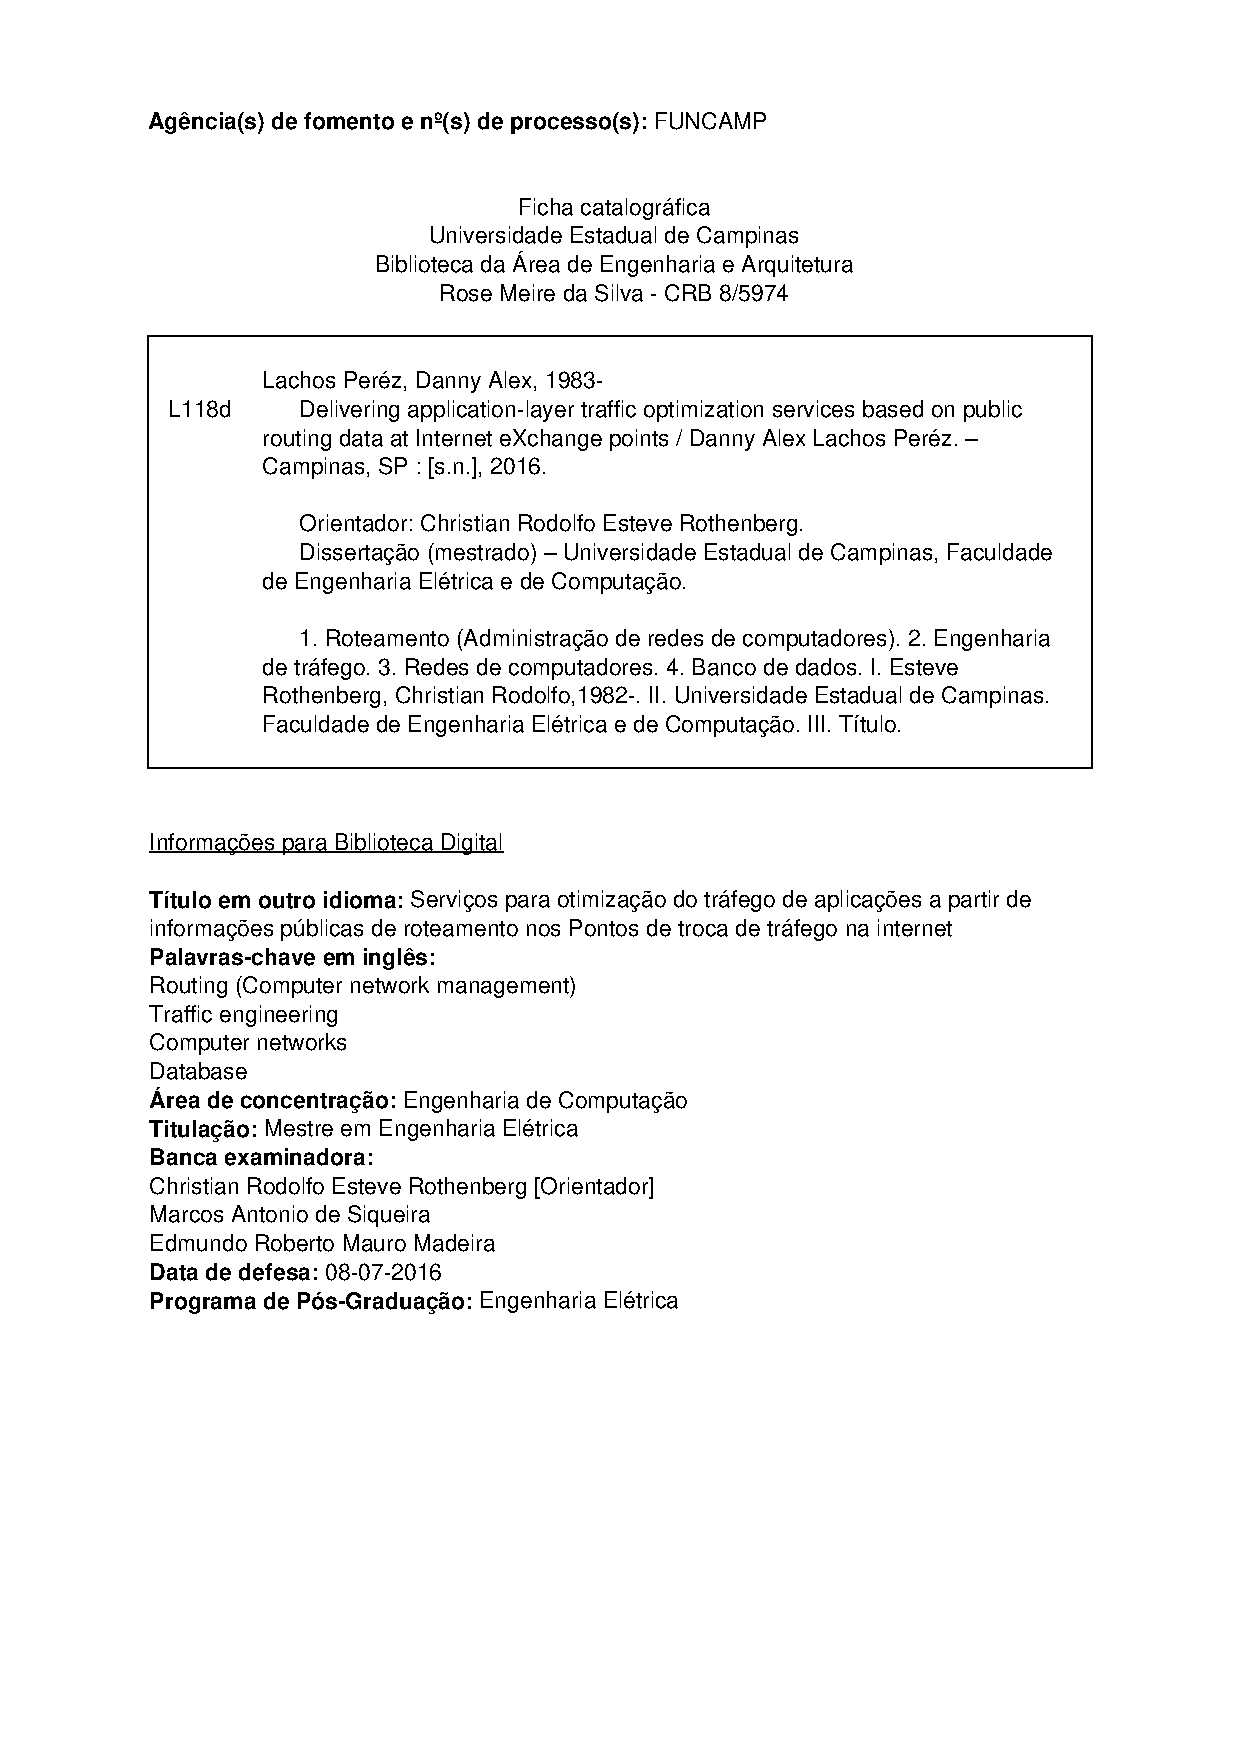
\includepdf[pages={1}]{docs/Ficha-Catalografica-Protocolo-86219375.pdf}
    %
\includepdf[pages={1}]{figures/cat.jpg}
    %\includepdf{ficha-catalografica.pdf}
 \end{fichacatalografica}
% ---
\newpage
%\vspace*{\fill}
%\begin{center}
%    \textsc{Inclua aqui a folha de assinaturas.}
%\end{center}
\textbf{COMISSÃO JULGADORA - DISSERTAÇÃO DE MESTRADO}

\vspace{1cm}
\begin{flushleft}
\textbf{Candidato}: Anderson dos Santos Paschoalon \hspace{1cm}     RA: 083233 \\
\textbf{Data da Defesa}: \\
\textbf{Título da Tese}: \\
``Generation of Synthetic and Realistic Network Workload for Benchmarking and Tests of Emerging Techinologies''\\%english\\
``Geração de Trafego de Rede Sintético e Realistico para Benchmarking e testes de Tecnologias Emergentes''%portuguese
\end{flushleft}
\vspace{0.2cm}
\begin{flushleft}Prof. Dr. Christian Rodolfo Esteve Rothenberg (Presidente, FEEC/UNICAMP)\\
Prof. Dr. Edmundo Roberto Mauro Madeira (IC/UNICAMP) - Membro Titular\\
Prof. Dr. Marcos Antonio de Siqueira (PADTEC) - Membro Titular
\end{flushleft}
\vspace{0.2cm} 
\begin{flushleft}Ata de defesa, com as respectivas assinaturas dos membros da Comissão Julgadora, encontra-se no processo de vida acadêmica do aluno. \end{flushleft}

%\vspace*{\fill}
\newpage
% --- --- ---
%\includepdf[pagecommand={\thispagestyle{plain}}]{folha-assinaturas.pdf}	
%\cleardoublepage
% --- Dedicat\'{o}ria ---
\begin{dedicatoria}
\vspace*{\fill}
\centering
\noindent
\textit{Mauris malesuada egestas enim, ac interdum justo feugiat quis. Etiam ullamcorper volutpat ex, at laoreet mauris vehicula eu. Integer dignissim egestas purus, sit amet feugiat orci fringilla vel. Curabitur tincidunt ac massa non molestie. Suspendisse potenti. In molestie a tortor ac pellentesque. Cras a risus et tellus hendrerit pretium ut quis arcu.}

\textit{Aliquam vehicula erat eu odio mollis, ut vehicula mauris laoreet. Cras volutpat ante sed orci bibendum maximus. Pellentesque felis elit, laoreet vitae bibendum in, malesuada ut nulla. Vestibulum pharetra faucibus blandit. Morbi tristique at leo ut ultrices. Etiam sollicitudin justo lacus, non rutrum mi imperdiet non. Cras nec mauris odio. Quisque eleifend purus interdum nulla suscipit lobortis.}

\textit{Proin vel nulla scelerisque nunc vehicula tempor. Curabitur non arcu ante. Etiam eget mattis tellus. Aenean molestie cursus ex, in pharetra eros hendrerit nec. In cursus egestas interdum. Ut scelerisque fringilla maximus. In facilisis vel dui vitae hendrerit. Integer a orci vel lectus lobortis fringilla. Phasellus eleifend commodo justo, cursus vehicula lorem. Donec a libero ultrices risus tempus condimentum imperdiet eget justo. 
}

\vspace*{\fill}
\end{dedicatoria}
% ---
% --- Agradecimentos ---
\begin{agradecimentos}
	%\lipsum[3]
%First of all, I would like to thank my advisor Prof. Dr. Christian Rothenberg for the trust and for letting me be part of his selected group of students. I would not be able to imagine the undertaking of this research without his innovative ideas, consistent support and continuous encouragement. I would therefore like to express my gratitude for being a great instructor and an even greater friend. 

%At the State University of Campinas (Unicamp) I have had the opportunity to learn from the best professors. I would like to acknowledge Prof. Dr. Mauricio Magalhães, Prof. Dr. Edson Borin, Prof. Dr. Edmundo Madeira and Prof. Dr. Léo Pini for sharing their knowledge and experience, which served as a constant motivation throughout this work.

%I would like to thank the committee members Marcos Antonio de Siqueira, Edmundo Roberto Mauro Madeira and Christian Rothenberg for the recommendations and insightful criticism they offered me in order to improve the final version of my thesis.

%I had the good fortune to meet very talented people within the INTRIG and LCA groups. My special thanks go to Mateus, Samuel, Samira, Gyanesh, Alex, Luis, Raphael, Anderson, Hirley, Ramon, Alaelson, Claudio, Talita, Javier, Elias, Rodrigo, Roberto, Mariana, Ranyeri, Aldo, Wallace, Vitor, Raphael V. and Amadeu, Mariana and Lino for their friendship and their support throughout these two years.

%I would like to express special gratitude for the financial and technical support received from the Ericsson Innovation Center (Brazil), which allowed me to carry out this research.    

 Mauris malesuada egestas enim, ac interdum justo feugiat quis. Etiam ullamcorper volutpat ex, at laoreet mauris vehicula eu. Integer dignissim egestas purus, sit amet feugiat orci fringilla vel. Curabitur tincidunt ac massa non molestie. Suspendisse potenti. In molestie a tortor ac pellentesque. Cras a risus et tellus hendrerit pretium ut quis arcu.

Aliquam vehicula erat eu odio mollis, ut vehicula mauris laoreet. Cras volutpat ante sed orci bibendum maximus. Pellentesque felis elit, laoreet vitae bibendum in, malesuada ut nulla. Vestibulum pharetra faucibus blandit. Morbi tristique at leo ut ultrices. Etiam sollicitudin justo lacus, non rutrum mi imperdiet non. Cras nec mauris odio. Quisque eleifend purus interdum nulla suscipit lobortis.

Proin vel nulla scelerisque nunc vehicula tempor. Curabitur non arcu ante. Etiam eget mattis tellus. Aenean molestie cursus ex, in pharetra eros hendrerit nec. In cursus egestas interdum. Ut scelerisque fringilla maximus. In facilisis vel dui vitae hendrerit. Integer a orci vel lectus lobortis fringilla. Phasellus eleifend commodo justo, cursus vehicula lorem. Donec a libero ultrices risus tempus condimentum imperdiet eget justo. 
    
    
\end{agradecimentos}

% ---
% --- Ep\'{\i}grafe  ---
\begin{epigrafe}
	\vspace*{\fill}
\begin{flushright}
\begin{minipage}{9.9cm}
\textit{``Discipline, sooner or later, will defeat intelligence.''\\
``A disciplina cedo ou tarde vencerá a inteligência.''\\
``La disciplina tarde o temprano vencerá a la inteligencia.''}
\end{minipage}
\end{flushright}

\begin{flushright}
\textit{Japanese proverb}
\end{flushright}
\end{epigrafe}

% ---
% --- RESUMOS (em portugu\^{e}s e ingl\^{e}s ---

\begin{resumo}
%\lipsum[1]

 Lorem ipsum dolor sit amet, consectetur adipiscing elit. Donec dignissim nulla vel interdum maximus. Curabitur diam turpis, tincidunt sit amet dolor ac, egestas gravida lorem. Maecenas ac varius lorem. Vivamus porta neque eros, a molestie augue fermentum sit amet. Duis ut pellentesque metus. In sollicitudin placerat risus. Phasellus auctor ac arcu ac sagittis. Pellentesque nec iaculis eros. Vivamus quis convallis felis, nec facilisis risus. Suspendisse potenti. Etiam luctus elit eu est fermentum auctor. Curabitur mattis, nulla quis posuere iaculis, dolor lectus euismod eros, eu commodo felis nunc sed tortor. Quisque aliquam leo diam, nec placerat sapien placerat et. Integer vel accumsan mauris.

Nam sodales purus ac nibh maximus, non tempor ante sagittis. Donec vulputate vehicula dapibus. Duis mollis nisl vel fermentum eleifend. Nam sollicitudin metus vitae justo bibendum ullamcorper. Mauris sollicitudin, tellus nec placerat rutrum, est lectus commodo enim, in imperdiet est elit sit amet justo. Integer scelerisque gravida facilisis. Aenean rhoncus eget metus id rutrum. Curabitur vel volutpat quam, id lobortis lectus. Aenean semper semper massa, at finibus eros varius eget. Etiam volutpat tellus est, at rhoncus ligula scelerisque sed. Sed nisi sapien, semper in pharetra eget, pellentesque ac dolor.

In at rhoncus mauris, non semper turpis. Praesent iaculis lorem faucibus interdum vehicula. Nullam nec massa feugiat, pharetra turpis vitae, dignissim eros. Aliquam vel sapien et risus vulputate luctus non at risus. Quisque ac urna massa. Donec faucibus diam eu ex egestas viverra. In feugiat nunc at erat convallis aliquam. Suspendisse consequat urna quam, non dignissim massa pretium vel. Donec tincidunt pellentesque vestibulum. Sed aliquet imperdiet libero a fringilla. Maecenas tempor augue vel accumsan imperdiet. Pellentesque accumsan quis risus non malesuada. Maecenas sodales suscipit libero, fringilla imperdiet augue elementum non. Integer dignissim vehicula libero vel volutpat. Cras vel molestie tellus, ac varius nunc. 

%Application-Layer Traffic Optimization (ALTO) is a recently standardized protocol that provides abstract network topology and cost maps in addition to endpoint information services that can be consumed by applications in order to become network-aware and to take optimized decisions regarding traffic flows. 
%In this work, we propose a public service based on the ALTO specification using public routing information available at the Brazilian Internet eXchange Points (IXPs).
%Our ALTO server prototype takes the acronym AaaS (ALTO-as-a-Service) and is based on over 2.5GB of real BGP data from the 25 Brazilian IX.br public IXPs.
%We evaluate our proposal in terms of functional behaviour and performance via proof-of-concept experiments, which point to the potential benefits of applications being able to take smart endpoint selection decisions when consuming the developer-friendly ALTO APIs.

\vspace{\onelineskip}

\noindent\textbf{Keywords}: Routing (Computer network management); IXPs (Internet exchange points); Computer networks; SDN (software defined networking).
    
%\cleardoublepage
%    \vspace{\onelineskip}
%    \vspace{\onelineskip}
\newpage
\begin{otherlanguage*}{english}
\begin{center}{\ABNTEXchapterfont\huge Resumo}\end{center}
    %\lipsum[2]
     Aliquam velit metus, elementum a metus a, pharetra molestie enim. Nam et dolor blandit, egestas libero ut, porttitor sem. Proin felis lorem, ultrices vel lacus eget, dapibus ornare urna. Donec et nibh ut orci condimentum cursus feugiat aliquet enim. Donec vel purus semper, iaculis dolor vel, placerat elit. Pellentesque nec magna pretium, eleifend risus eget, dapibus elit. Nam finibus sem at mauris auctor, a sodales erat bibendum. Phasellus mattis purus vel magna dignissim auctor. Sed at arcu a arcu hendrerit viverra ut a ligula. Sed et libero nibh. Sed sit amet nunc urna. Fusce eu arcu sed urna congue dapibus. Sed accumsan eget sem vitae euismod. Nulla lorem magna, viverra sit amet blandit vitae, accumsan et ante. Nunc ultrices eleifend pulvinar.

Vivamus nisi turpis, venenatis ut massa at, porttitor ornare tortor. Quisque tristique quam non nibh posuere pellentesque. Integer egestas felis ligula, ac rutrum turpis lobortis a. Donec scelerisque non sem porta scelerisque. Etiam molestie, arcu sagittis placerat fringilla, orci lacus lobortis odio, porttitor vehicula ex risus et velit. Sed tempor interdum volutpat. Sed ac dui eget justo convallis auctor. Duis lobortis mauris lacus, eu gravida ex hendrerit non. Nullam rutrum pretium nibh, id mollis est condimentum nec. Maecenas tincidunt erat sit amet mauris tristique, quis sagittis justo lobortis. Duis augue quam, semper eget ligula id, sagittis condimentum augue. Curabitur tincidunt scelerisque sollicitudin. 

%Otimização de Tráfego na Camada de Aplicação (ALTO - \textit{Application-Layer Traffic Optimization}) é um protocolo recentemente padronizado que fornece uma topologia da rede e mapa de custos abstratos, além de serviços de informação de endpoints que podem ser consumidos pelos aplicativos, a fim de tornar-se conscientes da rede e tomar decisões otimizadas sobre os fluxos de tráfego.
%Neste trabalho, propomos um serviço público baseado nas especificações ALTO usando informação de roteamento pública disponível nos Pontos de Troca de Tráfego (PTTs) brasileiros.
Nosso protótipo de servidor ALTO, representado pela sigla AaaS (ALTO-as-a-Service), é baseado em mais de 2,5 GB de dados BGP reais dos 25 PTTs públicos brasileiros (IX.br).
%Nossa proposta é avaliada em termos de comportamento funcional e desempenho através de experimentos de prova de conceito que apontam como potencial benefício das aplicações, a capacidade de tomar decisões inteligentes na seleção de endpoint ao consumir as APIs ALTO.
\vspace{\onelineskip}
\noindent\textbf{Palavras-chaves}: Roteamento (Administração de redes de computadores); Engenharia de tráfego; Redes de computadores; Bancos de dados.

\end{otherlanguage*}
\end{resumo}
% ---

% --- inserir lista de ilustra\c{c}\~{o}es ---
\pdfbookmark[0]{\listfigurename}{lof}
\listoffigures*
\newpage
%\cleardoublepage
% ---

% --- inserir lista de tabelas ---
\pdfbookmark[0]{ \listtablename}{lot}
\listoftables*
\newpage
% ---
%\printglossary
%\cleardoublepage

\printglossary[type=\acronymtype]
\newpage
% --- inserir o sumario ---

\pdfbookmark[0]{\contentsname}{toc}
\tableofcontents*
\cleardoublepage
% ---

%\input{acronyms}
%\renewcommand{\nomname}{Acronyms and Abbreviations List}
%%\pdfbookmark[0]{\nomname}{las}
%\printnomenclature
\cleardoublepage
% ---
% CORRECTIONS 16-11
\pagenumbering{arabic}
\setcounter{page}{17}

% ---- ELEMENTOS TEXTUAIS ----
\textual

% ---- Introdu\c{c}\~{a}o ----
%\label{cap:intro}
%%%%%%%%%%%%%%%%%%%%%%%%%%%%%%%%%%%%%%%%%%%%%%%%%%%%%%%%%%%%%%%%%%%%%%%%%%%%%%%%
\chapter{Introduction}\label{ch:introduction}
%%%%%%%%%%%%%%%%%%%%%%%%%%%%%%%%%%%%%%%%%%%%%%%%%%%%%%%%%%%%%%%%%%%%%%%%%%%%%%%%

%3nd-review
\section{Motivation}
 

Emerging technologies such as SDN and NFV can be considered great promises that would drastically change the development and operation of computer networks. However, its enabling technologies such as virtualization still pose challenges as for performance,  reliability, and security\cite{nfv-challenges}. Closed hardware solutions are easier to pass on Service Layer Agreement since they have a much more predictable behavior. Since it is expected that virtualization will affect performance negatively, these VNFs have to keep their degradation as small as possible. Therefore, guaranteeing the Service Layer Agreements becomes now a harder question. There is a demand for more reliable methods to ensure SLAs, over different types of loads.


It is already a well-known fact that the type of traffic used on performing tests matters. Studies show that  realistic Ethernet traffic provides different and variable load characteristics on routers\cite{harpoon-validation}, even with the same average bandwidth consumption. This fact indicates that tests that employ constant bit rate traffic generator tools are not enough for a complete validation of new technologies. There are many reasons for this behavior, which includes a grater traffic burstiness and variable packet sizes.


A burstier traffic can cause packet losses and buffer overflows on network \cite{burstiness-queue-lenght} \cite{modelling-of-self-similar} \cite{empirical-interarrival-study}; thus degenerating network performance\footnote{Packet-trains periods and inter-packet times affect traffic burstiness}, and  measurement accuracy\cite{legotg-paper} \cite{background-traffic-matter}. Another key question is how applications will deal with packets, since it is a well-known fact that applications have a huge performance degradation in processing small packets\cite{comparative-trafficgen-tools}. A realistic synthetic traffic must not have a single one but rater use variable packet sizes \cite{packet-distribution-model}. 


Furthermore realistic workload generators are an essential security research\cite{ditg-paper}, since generation of realistic workloads is important for evaluation of firewall middleboxes. It includes studies of intrusion, anomaly detection, and malicious workloads\cite{ditg-paper}. Over a virtualized enviroment a realistic workload is expected to have an even larger inpact.


Another critical point is the flow-oriented operation of SDN networks, in which each new flow arriving on an SDN switch demands an extra communication with the controller, that may cause a bottleneck. Since its operation relies on queries on flow tables, a stress load must have the same flow properties of an actual Internet Service Provider. Therefore, there is a demand for the study of the impact of a realistic traffic on this new sort of environment. How VNFs and virtualized middle-boxes and SDN testbeds will behave if stressed with a realistic traffic load in comparison to a constant rate traffic is a relevant subject.



\section{Related Work}


The open-source community offers a huge variety of workload generators and benchmarking tools \cite{ditg-paper}\cite{validate-trafficgen}\cite{comparative-trafficgen-tools}\cite{performance-trafficgen}. Most of these tools were built for specific purposes and goals, so that each uses different methods of traffic generation, and enable controll of different features, such as: bits/bytes per second; packets per seconds; packet-sizes; protocols, header or payload customization; inter-packet times and On/Off periods; starting and sending time; and emulation of applications, such as Web server/client communication, VoIP, HTTP, FTP, p2p applications, and many more.


Some traffic generator tools offer support emulation of single application workloads, however, this does not correspond to real complex scenarios. Other tools work as packet replay engines, such as TCPreplay and TCPivo. While is possible to produce a realistic workload at high rates using this tools, they comes with some drawbacks. Firstly, the storage space required becomes huge for long-term and high-speed traffic capture traces, lastly, obtaining good traffic traces is sometimes hard, due privacy issues and fewer good sources. 


Many tools support a larger set of protocols and high-throughput for traffic generation, such Seagull and Ostinato. Others are also able to control inter-packet times and packet sizes using stochastic models, like D-ITG\cite{ditg-paper}, sourcesOnOff\cite{sourcesonoff-paper}, and MoonGen. All of them offer a complex configuration framework, but its custumization is all up to the user. So, there is no simple way for the user to create a synthetic and realistic traffic scenario. 

We also have a variety of APIs that enable the creation of traffic and custom packets, which include low-level APIs, such as Linux Socket API,  Libpcap, Libtins, DPDK, Pcapplusplus, libcrafter, impacket, scapy and many others. These APIs provide a finer controll and customization over each packet, and are used to implement traffic generators. For example, Ostinato and TCPreplay uses Libpcap, and MoonGen uses DPDK. In addition, many of the listed traffic generators provides their own API, such as Ostinato Python API, D-ITG C API, and MoonGen LUA API. 



%They can give a good control of the traffic and high rates. Es example of controllable features we can list:
%\begin{itemize}
%\item Throughput, the number of bytes, number of packets.
%\item Protocols. Most of the tools give support to network and transport protocols. Many also offer support to Link and Application protocols;
%\item Header and payload configuration. Support for header customization includes source and destination port/addresses, QoS parameters, flags, etc. Some traffic generators also allow customizing payload bytes.
%\item Inter-packet times. Some tools offer a set of stochastic distributions to control inter-packet times. The user can use these stochastic functions to emulate realistic inter-arrival times.
%\item On/off periods: support of packet trains periods. Many offer stochastic models to control it. 
%\item Sending time and start-time: the user can use these features to control flows timings.  
%\item Packet-size: support for different packet sizes. Some tools offer constant values or stochastic distributions to control packet sizes.
%\item Paralell flows configuration.
%\item Emulation of specific applications: common examples are 
%\end{itemize}


There is a  have a large variety of open-source tools available for custom traffic generation, but reproducing a realistic traffic scenario is a hard matter. Selecting the right framework, a good traffic model, and the right configuration, is by itself a complex research project\cite{legotg-paper}\cite{selfsimilar-ethernet}. Since it usually is not the main goal of the project, but just a mean of validation, many times a simplistic and unrealistic solution is selected due the limited resources such as time and labor.  Creating a realistic traffic through these tools is a manual process and demands implementation of scripts or programs leveraging human (and scarce) expertise on network traffic characteristics  and experimental evaluation. 


There are few solutions on the open source community available that aiming to fill this gap, such as Harpoon\cite{harpoon-paper} and Swing\cite{swing-paper}.They capture traces to set internal parameters, providing an easier configuration. However they have their issues as well. Harpoon does not configure parameters at packet level\cite{harpoon-paper} and is not supported by newer Linux kernels, what may be a huge problem with setup and configuration. Swing\cite{swing-paper} aims to generate realistic traffic, but focous on background traffic; so throughputs it is not a goal off the application\cite{swing-paper} \cite{legotg-paper}. ecause its traffic generation engine is coupled to its modeling framework, you cannot opt to use a newer/faster packet generation library. The only way of replacing the traffic engine is changing and recompiling the original code which is a hard and  error prone activity\cite{legotg-paper}. Again, we fall in the same issue, a complex task that is usually not the goal of the project. In the table ~\ref{tab:related-work} we give a brief summary of what we have available on some open-source traffic-generators tools. 

% Another matter is the large variety of tools, and different methods of configuration and its limitations. To create a custom traffic, a user must read large manuals, and custom-design scripts. One of our bigger proposals is create a tool able to automatically do this processes. So The user may design his custom traffic by creating his own Compact Trace Descriptor, and create a traffic using many different tools, like Ostinato, D-ITG, Iperf, but not caring about how to proper configure each of them. In the table ~\ref{tab:related-work} we summarize our current scenario.



\begin{table}[ht!]
	\centering
	\caption{Current scenario of traffic generation}
	\scalebox{0.87}{
	\begin{tabular}{cccccc}
		\hline
		\rowcolor[HTML]{9B9B9B} 
		Solution    & User Space  & Autoconfigurable & Realistic Traffic & Traffic Custumization & Extensibility \\ \hline
		Harpoon      & \textbf{no} & yes              & yes               & yes                   & \textbf{no}   \\
		\rowcolor[HTML]{C0C0C0} 
		D-ITG        & yes         & \textbf{no}      & yes               & yes                   & \textbf{no}   \\
		Swing        & yes         & yes              & yes               & \textbf{no}           & \textbf{no}   \\
		\rowcolor[HTML]{C0C0C0} 
		Ostinato     & yes         & \textbf{no}      & \textbf{no}       & yes                   & yes           \\
		LegoTG       & yes         & \textbf{no}      & \textbf{no}       & yes                   & yes           \\
		\rowcolor[HTML]{C0C0C0} 
		sourcesOnOff & yes         & \textbf{no}      & yes               & yes                   & \textbf{no}   \\
		Iperf        & yes         & \textbf{no}      & \textbf{no}       & yes                   & \textbf{no}   \\ \hline
	\end{tabular}
	}
	\label{tab:related-work}
\end{table}

%Since synthetic traffic traces generation is mature in academia, the creation of custom network workloads through the configuration of  open-source tools is an affordable task. But it is not often available in an automatic way, and most of the times is a challenging question\cite{legotg-paper}, and still, requires expert knowledge. It requires time, study, and is vulnerable to human mistakes and lack of validation. Such work may require weeks to complete a realistic reproduction of a single scenario, so most of the time it is just not done. We argue that widely (i.e. affordable) existing approaches can be regarded as simplistic often point solutions to more general cases. 


% Also, just choosing which workload generator tool may fit better for the user needs is not a simple question. Tools like D-ITG\footnote{\href{http://traffic.comics.unina.it/software/ITG/}{http://traffic.comics.unina.it/software/ITG/}} provide support to many different stochastic functions, Ostinato\footnote{\href{http://ostinato.org/}{http://ostinato.org/}} provides a larger support for protocols, and a higher throughput for each thread\cite{comparative-trafficgen-tools}, and others like Seagull\footnote{\href{http://gull.sourceforge.net/doc/WP_Seagull_Open_Source_tool_for_IMS_testing.pdf}{http://gull.sourceforge.net/doc/WP\_Seagull\_Open\_Source\_tool\_for\_IMS\_testing.pdf}} are responsive. 


\section{Problem Statement}


Based on what we stated,  we are going to formalize our research targets, and define que requet list to fulfill these gaps. Our main research targets in this work are:

\begin{itemize}
	
	\item Survey open-source Ethernet workload tools, addressing different features of each one. In this step, we want to evaluate the existing solution ready to use for network researchers and developers, and what can be used and integrated into our project as part of our solution;
	
	\item Define what a realistic Ethernet traffic is, and a set of metrics to measure the realism and the similarity between an original and a synthetic traffic.
	
	\item Research the main apporoaches and methods found of the literature for realistic traffic generation. 
	
	\item Create a general method for modeling and parameterization of Ethernet traffic;
	
	\item Create a self-configurable tool that observes and uses real network traffic, and try to mimic and reproduce its behavior characteristics, \textit{avoiding} the storage of \textit{pcap} files.
	
\end{itemize}

Hence, we will define a requeriment list for the tool we are going to develop and present in this research:

\begin{itemize}
	
	\item Autoconfigurable: It must be able to extract data from a real traffic and store in a database, and use it to parametrize its traffic model. It must be able to obtain data from real-time traffics and from \textit{pcap} files;
	
	\item Technology independent: It must have a flow-based abstract model for traffic generation, not attached to any specific technology.
	
	\item Human readable: it must produce a human-readable file as output that describes our traffic using our abstract model. We call this file a Compact Trace Descriptor;
	
	\item Extensibility: the traffic modeling and generation must be decoupled. Ideally, it must able to use as traffic generator engine any library or traffic generator tool;
	
	\item Simple usage: It must be easy to use. It has to take as input a Compact Trace Descriptor, just as a traffic replay engine (such as TCPreplay) would take a \textit{pcap} file;
	
	\item Traffic generation programmability: It must have what we call \textit{traffic generation progamability}. The compact trace descriptor must be simple and easy to read. That way, the user may want to create his custom traffic, in a platform agnostic way. The traffic programmability must be flow-oriented;
	
	\item Flow-oriented: The traffic modeling and generation must be flow-oriented. Each flow must be modeled and generated separately.
	
\end{itemize}







%These targets summarize a target of research, based on what we have exposed until now. We also will define some extra features, we want to have on our tool:
%\begin{itemize}
%\item Traffic Flow Programmability: the tool records this parameterization on a light-weight and human-readable version of a \textit{pcap} file. So the user can create his own models of traffic based on flows, in a platform-independent manner. He will not have to learn how to configure and script each tool.
%\item Easy expansion: The sniffing, modeling, and traffic generation processes must work separately, so updates will be easy to manage. Also, the traffic generation is flow-oriented (it generates each flow individually). Thus the scheduling of each flow is platform-independent. In this way, is much easier to expand the support for new traffic generation engines.
%\end{itemize}


%Now, we are going to formalize these exposed concepts in a proposal of research and development. Or main targets here are:
%\begin{itemize}
%\item Survey the available open-source Ethernet workload tools available, addressing its different features;
%\item Define what is a realistic Ethernet traffic, and the man approaches found in literature;
%\item Create a general method for modeling and parameterization of Ethernet traffic, aiming to mimic a provided input;
%\item Create a software \textit{tool} able of \textit{learning} patterns and characteristics of real network traffic traces, and auto-configure the network traffic workloads, allowing to reproduce network traffic with similar (but not equal) characteristics, avoiding storage of \textit{pcap} files. 
%\item It must have a flow-oriented operation, and be able to choose the best features to represent each flow traffic. It will generate realistic Ethernet traffic based on these features learned, using available open source tools and APIs;
%\end{itemize}

%We also aim some advantages from the addition features: data visualization, packet acceleration, and distributed operation. Providing data visualization, it will not just work as a workload generator, but as a benchmark tool, providing statistics and performance analysis. Using packet acceleration, we will be able to produce a high throughput at the wire, and at the same time generate a trace as realistic as possible. Through a distributed operation of multiple instances, it will be easier to control its operation in a virtualized environment.  Finally, a project guideline is to reuse as much code and components as possible from the open-source community.



\section{Document Overview}


In this introductory chapter, we presented an abstract of state of the art, a problem statement, and proposed an approach for research and requirements for development.

%2nd-review
In the chapter section~\ref{ch:literature-review}, we go more in-depth on some subjects mentioned here. First, we present an extensive survey on open-source traffic generator tools. We summarize the benefits, and features supported by each one. After, we offer a brief review of essential topics on realistic traffic generation. We are defining some central concepts we are going to use in this work, such as self-similarity, and heavy-tailed functions. Then, we discuss some techniques of validation of traffic generator tools and some practical examples. We also will analyze some related works. 

%2nd-review
Chapter ~\ref{ch:architecture} introduces the methodology used in our project. We describe \textit{SIMITAR} low-level requirements and define an architecture and their algorithms.  We also present its classes design and explain how \textit{SIMITAR} we can expand to any traffic generator engine or library, with an API, CLI interface. We use the Iperf as an example. We explain its operation and suggest some use cases.

%2nd-review
In the chapter~\ref{ch:modeling-evaluation} we go deep in some subjects pointed in the previous chapter. We present how the modeling process works, using a defined data set (which we are going to use in the rest of the work). We also show some evaluation methods to check the modeling quality. We also describe our used and developed algorithms.

%2nd-review
In the chapter ~\ref{ch:validation}, we define a set of metrics based on previous tests on validation of traffic generators found in the literature. Here, we focus on packet, flow, and scaling metrics. we test \textit{SIMITAR} in an emulated SDN testbed with Mininet, using OpenDayLight as controller\cite{web-opendaylight}. 

% On chapter Use Cases~\ref{ch:use-cases}, we present two use cases of our tool. One using an NFV testbed, and other handling an SDN p4 switch. Here we focus on QoS metrics, such as mean RTT. %use tools such as Tcptrace and NFPA  on the use cases

% 2nd-review
Finally, on chapter Conclusion and Future Work~\ref{ch:conclusion}, we summarized our work and highlighted future actions to improve \textit{SIMITAR} on realism and performance.


%%%%%%%%%%%%%%%%%%%%%%%%%%%%%%%%%%%%%%%%%%%%%%%%%%%%%%%%%%%%%%%%%%%%%%%%%%%%%%%%
\chapter{Literature Review}\label{ch:literature-review}
%%%%%%%%%%%%%%%%%%%%%%%%%%%%%%%%%%%%%%%%%%%%%%%%%%%%%%%%%%%%%%%%%%%%%%%%%%%%%%%%

%2nd-review
In this chapter, we will review some topics from the literature that serve as a base for this whole work. First of all, we will define what is a traffic generator tool, and introduce a taxonomy that distinguishes them. After this, we will present a survey of many available open-source and free traffic generators. We introduce each tool and present a feature comparison between each of them. As far as we know, this is the extensible features comparison of traffic generators available so far in the literature. The first two sections are devoted for this topic.

%2nd-review
We also will overview network traffic modeling and realistic traffic generation. We will discuss stochastic models that used to describe the Internet traffic. Based on that we will discuss what features a realistic traffic should have and highlight important features needed to control to achieve it.  We can count self-similarity and burstiness,  header fields, packet size and flow features.

%2nd-review
In the following section, we will make a brief discussion on validation of traffic generator tools. First, presenting the main approaches of validation made on literature. Then, we will discuss some validation study cases of related works, always introducing new concepts when needed.

%Finally, we will present a short overview of new arriving network technologies: SDN and NFV. We will use them as use cases at the chapter ~\ref{ch:use-cases}. Also, we will present our motivations for this choice. 

%%%%%%%%%%%%%%%%%%%%%%%%%%%%%%%%%%%%%%%%%%%%%%%%%%%%%%%%%%%%%%%%%%%%%%%%%%%%%%%%
\section{Traffic generator tools}

%2nd-review
A traffic generator tool is a system capable of creating and injecting packets into a computer network in a controlled way to generate a synthetic traffic \cite{validate-trafficgen}.  there is a huge variety of traffic generation tools described on the literature \cite{validate-trafficgen} \cite{ditg-paper} and available i the open-source community\footnote{\href{http://www.icir.org/models/trafficgenerators.html}{http://www.icir.org/models/trafficgenerators.html}}. In fact, as exposed in the chapter~\ref{ch:introduction} it is a hard task to find what is the best tool for your needs. This is a cause of many  different approaches and methodologies available to network traffic generator's developers \cite{validate-trafficgen}.

%2nd-review
%Also, previous research such as Oliver et al. \cite{flow-level-ip} have demonstrated that one unique statistical law cannot express all complexity of an original Internet trace (an Internet trace is an Internet traffic capture made over a network interface). So, just selecting a stochastic process for a traffic generator, do not guarantee realism.

%2nd-review
New network generators development is directly related with to the current needs of network environment, applications sets, and purpose of use \cite{validate-trafficgen}. According to the context, you may want to send as many packets as possible through an interface to  equipment stress . So, in this case, a maximum throughput traffic generator is more interesting. In others situations, you may want a stochastically realist profile. Or even a traffic generator that reflect a special scenario such as a specific application; for example a client and server exchanging data\cite{surge-paper}. In this case, the target would be to stress a server, not an equipment. Another possibility a huge variety of protocols available, or even support of new protocols.

%2nd-review
Alongside with the traffic generators, there are many APIs available. There are low-level APIs which enables direct packet injection and capture, such as \textit{libpcap}\cite{web-tcpdump}, \textit{libtins}\cite{web-libtins}, DPDK\cite{web-dpdk} and the GNU C socket library\cite{web-socket}. And there are high-level APIs, provided by traffic generator tools, such as D-ITG\cite{ditg-paper}, Ostinato\cite{web-ostinato} and MoonGen\cite{moongen-paper}. In this case they enable an easy custom traffic generation and statistics. Also, there are implementations of hardware-based traffic generators using NetFPGAs\footnote{\href{http://netfpga.org/site/\#/}{http://netfpga.org/site/\#/}}.

%2nd-review
In the literature there are many classifications of traffic generators\cite{sourcesonoff-paper}\cite{hybrid-traffic-gen}\cite{validate-trafficgen}\cite{do-you-trust}. Some tools may have some features compatible with one or more classes. But classify them it is an efficient way to distinguish the difference between these tools. We will give two different taxonomies:

%2nd-review
\begin{itemize}
\item According to its abstraction level \cite{do-you-trust};
%\item According to its purpose (engine replay, throughput, realism) \cite{validate-trafficgen}
\item According to its implementation.
\end{itemize}


%%%%%%%%%%%%%%%%%%%%%%%%%%%%%%%%%%%%%%%%%%%%%%%%%%%%%%%%%%%%%%%%%%%%%%%%%%%%%%%%
\subsection{Classes of traffic generator tools}

The most common traffic generator taxonomy found is  according to its abstraction level\cite{do-you-trust}. They are: Application-level/Special-scenarios, flow-level, packet-level and Closed-loop and multi-level traffic generators. We present a diagram  ilustrating its concept at figure ~\ref{fig:layers-workload-tools}.


\subsubsection{According to its abstraction level}

\textbf{Application-level/Special-scenarios traffic generators}: they try to emulate the behavior of network applications, simulating real workloads stochastically, responsively \footnote{Responsiveness refers to the property of capacity of response over time of the workload tool. That means, the behavior of the output may change according to what packets have arrived in the network interface} or both. As examples we have Surge\cite{surge-paper} able to emulate the behavior of web clients and services. The behavior of such applications is, in general, based on request-response exchanges models.



\textbf{Flow-level traffic generators}: they are able to configure and reproduce precisely features at the flow level\cite{do-you-trust}\cite{sourcesonoff-paper}, such as flow duration, start times distributions, and temporal (diurnal) traffic volumes\cite{do-you-trust}. Harpoon \cite{harpoon-paper} is able to extract these parameters from Cisco NetFlow data, collected from live routers.

\textbf{Packet-level traffic generators}: most traffic generators available fall in this class. They are able to craft packets and inject them into the network based on Inter departure times (IDT) and packet size(PS). \cite{validate-trafficgen} classify them as replay engines, maximum throughput generators, and model based generators. Traffic Replay engines, such TCPreplay\cite{web-tcpreplay}, are  able to read packet capture files (\textit{pcap} files), and inject copies on a network interface. Model-based generators, such D-ITG \cite{ditg-paper}, TG\cite{web-tg}, may have PS and IDT configured by the user. They can configure IDT  either by constant values (defining the packet rate or bandwidth) or by stochastic models. Maximum throughput engines like Ostinato and Seagull are tools that the main goal is to perform end-to-end stress testing. Are included in this category generators that are able to craft packets from the link layer, like Brute\cite{web-brute}, KUTE\cite{web-brute}, and pktgen\cite{web-pktgen}.

\textbf{Closed-loop and multi-level traffic generators}: this is a more recent class of network traffic generator, and its proposal is to take into account existing interaction among each layer of the network stack, to create background network traffic as close as possible from reality. One of the most relevant tools we can found is Swing \cite{swing-paper}. Swing take into account many points of each layer, using an approach based on randomness and responsiveness \cite{swing-paper}. That means, it uses PS and IDT stochastic models, but also take into account flow and application layer behavior. Swing is able to model things like\cite{swing-paper}: 
\begin{itemize}

\item User behavior: Number of request and responses, time between requests and responses;

\item Request and Responses: number of connections, time between start of connections;

\item Connection: Number of request and responses per connection, applications modeling (HTTP, P2P, SMTP), transport protocols TCP/UDP based on the application, response sizes, request sizes, user think between exchanges on a connection;

\item Packet: packet size (Maximum transmission unit), IP addresses, (MTU), bit rate and packet arrival distribution, 

\item Link: link Latency Delay, loss rates.


\end{itemize}

Swing take as input collected \textit{pcap} files. Botta at al. \cite{do-you-trust} argues that due its complexity, they are rarely used to conduct experimental researchers. Also, we can  justify due its overheads, since the performance of such complex traffic generator is limited\cite{legotg-paper}. The authors Vishwanat et al. \cite{swing-paper} cite that they have generated traces of about of 200 Mbps, about the same result found by \cite{legotg-paper}. In the other hand, D-ITG reached 9808 Mbps\cite{comparative-trafficgen-tools} in a link of 10 Gbps, but operating as a maximum throughput generator.g1



\begin{figure}[!ht]
	\centering
	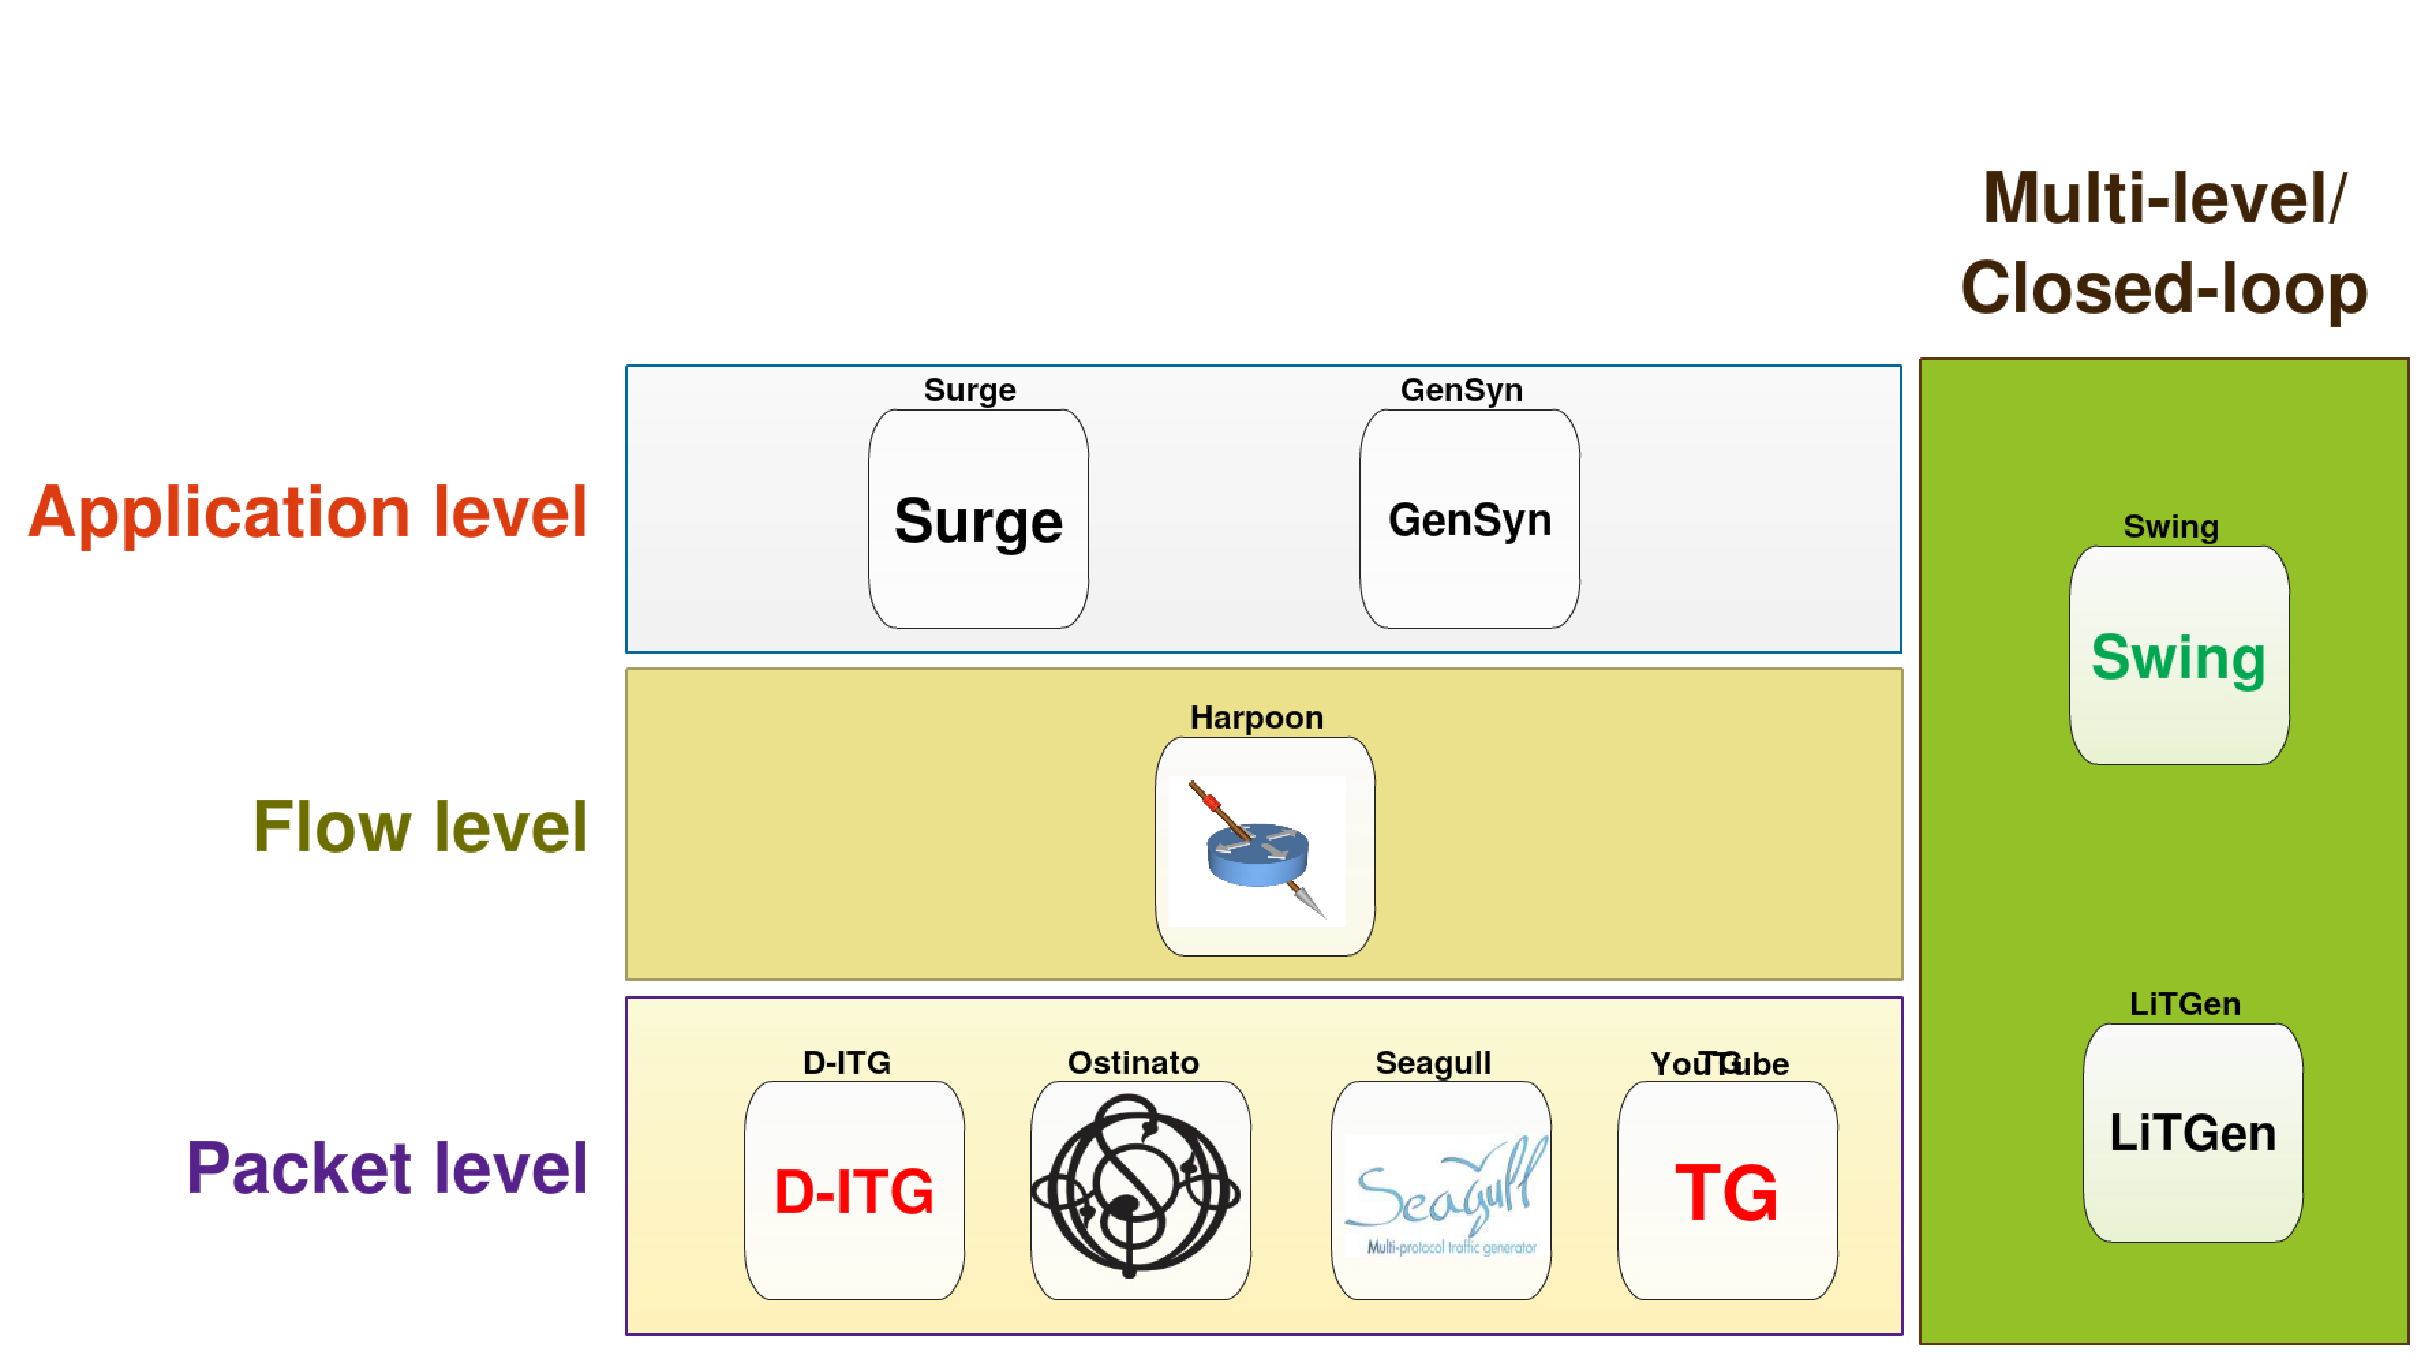
\includegraphics[scale=0.4]{figures/ch2/types-workload-tools}
	\caption{Diagram representing different traffic generators, according to its abstraction layer.}
	\label{fig:layers-workload-tools}
\end{figure}

\subsubsection{According to its implementation}

\textbf{Software-only traffic generators}: Implementations of traffic generators completely independent of its running hardware platform. This comprehends most of traffic generator tolls.

\textbf{Software and hardware-dependent traffic generators}: Traffic generators implemented in software, but dependent of underlying hardware. The most preeminent examples of this class are implemented over DPDK\cite{web-dpdk}. DPDK works directly on the NIC interface, avoiding overheads of the Operational System. As cited on its official website, this approach permits huge precision and speed in the timing of packets, since it is able to send and receive packets within less than 80 clock cycles.

\textbf{Hardware traffic generators}: This open-source traffic generators implementations are implemented in hardware description language (VHDL/Verilog), and work on NetFPGAs. Some examples of implementations are: PacketGenerator \cite{web-netfpgapacketgenerator}, Caliper \cite{web-caliper}, and OSNT Packet Generator \cite{web-osnt}.





%Tabela: revisao dos principais geradores de trafego
\renewcommand{\tabularxcolumn}[1]{>{\small}m{#1}}


\begin{table}[t!]
\caption{Review of features of some open-source traffic generators}
\begin{center}
\begin{footnotesize}
\begin{tabularx}{\linewidth}{
|>{\hsize=0.9\hsize\raggedright\arraybackslash}X	% 10% of 4\hsize 
|>{\hsize=1.16\hsize\centering\arraybackslash}X					% 30% of 4\hsize
>{\hsize=1.37\hsize\centering\arraybackslash}X					% 30% of 4\hsize
>{\hsize=1.16\hsize\centering\arraybackslash}X					% 30% of 4\hsize
>{\hsize=0.7\hsize\centering\arraybackslash}X					% 30% of 4\hsize
>{\hsize=0.7\hsize\centering\arraybackslash}X|					% 30% of 4\hsize
% sum=4.0\hsize for 4 columns
}
	\hline
	\textbf{Traffic Generator} & 
    \textbf{Operating System} & 
    \textbf{Protocols supported} & 
    \textbf{Stochastic distribution} & 
    \textbf{Interface} & 
    \textbf{Operation Level} \\
    
    \hline
    GenSyn	&
    Java virtual machine &
    TCP, UDP, IPv4 &
    (\textit{user model}, \textit{responsible}) &
    GUI &
    application-level \\
    			
    \hline
    Harpoon &
    FreeBSD 5.1-5.4, Linux 2.2-2.6, MacOS X 10.2-10.4, and Solaris 8-10 &
    TCP, UDP, IPv4, IPv6 &
    (\textit{flow-level model, based on a input trace})&
    CLI &
    flow-level\\    

    \hline
    D-ITG &
    Linux, Windows, Linux Familiar, Montavista, Snapgear &
    IPv4, IPv6, ICMP, TCP, UDP, DCCP, SCTP &
    Constant, uniform, exponential, pareto, cauchy, normal, poisson, gamma, on/off, \textit{pcap}&
    CLI, Script, API &
    packet-level \\
    
    \hline
    Ostinato &
    Linux, Windows, FreeBDS &
    Ethernet/802.3/LLC SNAP; VLAN (with QinQ); ARP, IPv4, IPv6, IP Tunnelling (6over4, 4over6, 4over4, 6over6);TCP, UDP, ICMPv4, ICMPv6, IGMP, MLD; HTTP, SIP, RTSP, NNTP etc... \textit{extensible}&
    constant &
    GUI, CLI, Script, API &
    packet-level\\
	 		
    \hline
    Seagull&
    Linux, Windows &
    IPv4, IPv6, UDP, TCP, SCTP, SSL/TLS and SS7/TCAP. \textit{extensible}&
    constant, poisson, \textit{responsible} &
    CLI, API &
    packet-level\\



    \hline
    PackETH &
    Linux, MacOS, Windows &
    ethernet II, ethernet 802.3, 802.1q, QinQ, ARP, IPv4, IPv6, UDP, TCP, ICMP, ICMPv6, IGMP &
    constant &
    CLI, GUI &
    packet-level \\ 

    \hline
    Iperf &
    Windows, Linux, Android, MacOS X, FreeBSD, OpenBSD, NetBSD, VxWorks, Solaris &
    IPv4, IPv4, UDP, TCP, SCTP &
    constant &
    CLI &
    packet-level \\ 
     
    \hline
\end{tabularx} 
\label{tab:trafficgen-list1}
\end{footnotesize}
\end{center}
\end{table} 
\clearpage

\begin{table}[t!]
\caption{Review of features of some open-source traffic generators}
\begin{center}
\begin{footnotesize}
\begin{tabularx}{\linewidth}{
|>{\hsize=0.9\hsize\raggedright\arraybackslash}X	% 10% of 4\hsize 
|>{\hsize=1.16\hsize\centering\arraybackslash}X					% 30% of 4\hsize
>{\hsize=1.37\hsize\centering\arraybackslash}X					% 30% of 4\hsize
>{\hsize=1.16\hsize\centering\arraybackslash}X					% 30% of 4\hsize
>{\hsize=0.7\hsize\centering\arraybackslash}X					% 30% of 4\hsize
>{\hsize=0.7\hsize\centering\arraybackslash}X|					% 30% of 4\hsize
% sum=4.0\hsize for 4 columns
}
	\hline
	\textbf{Traffic Generator} & 
    \textbf{Operating System} & 
    \textbf{Protocols supported} & 
    \textbf{Stochastic distribution} & 
    \textbf{Interface} & 
    \textbf{Operation Level} \\
   
    \hline
    Swing &
    Linux &
    IPv4, TCP, UDP, HTTP, NAPSTER, NNTP and SMTP &
    \textit{capture trace}  &
    CLI &
    closed-loop and multilevel \\     
   
    \hline
    BRUTE &
    Linux &
    IPv4, IPv6 &
    constant, poisson, trimoda &
    CLI &
    packet-level \\ 
    
         
    \hline
    SourcesOnOff &
    Linux &
    IPv4, TCP, UDP &
    on/off (Weibull, Pareto, Exponential and Gaussian) &
    CLI &
    packet-level \\      
     
     \hline
    TG &
    Linux, FreeBSD, Solaris SunOS &
    IPv4, TCP, UDP &
    Constant, uniform, exponential, on/off &
    CLI &
    packet-level \\ 
    
    \hline
    Mgen &
    Linux(Unix), Windows &
    IPv4, IPv6, UDP, TCP, SINK &
    Constant, exponential, on/off &
    CLI, Script &
    packet-level \\ 

     
     \hline
    KUTE &
    Linux 2.6 &
    UDP &
    constant &
    kernel module &
    packet-level \\ 
     
     \hline
    RUDE \& CRUDE &
    Linux, Solaris SunOS, and FreeBSD &
    IPv4, UDP &
    constant &
    CLI &
    packet-level\\      

     
     \hline
    NetSpec &
    Linux &
    IPv4,UDP, TCP &
    uniform, Normal, log-normal, exponential, Poisson, geometric, Pareto, gamma &
    Script &
    packet-level \\ 
     
     \hline
    Nping &
    Windows, Linux, Mac OS X &
    TCP, UDP, ICMP, IPv4, IPv6, ARP &
    constant &
    CLI &
    packet-level \\ 
     
     
     \hline
    TCPreplay &
    Linux &
    \textit{pcap} &
    constant, \textit{pcap} &
    CLI &
    packet-level (\textit{replay engine}) \\ 

     
     \hline
    TCPivo &
    Linux &
    \textit{pcap} &
    constant, \textit{pcap} &
    CLI &
    packet-level (\textit{replay engine}) \\ 

     \hline
     NetFPGA PacketGenerator &
     Linux &
     \textit{pcap} &
     constant &
     CLI &
     packet-level (\textit{hardware-based}) \\ 

 

    \hline
\end{tabularx} 
\label{tab:trafficgen-list2}
\end{footnotesize}
\end{center}
\end{table} 
\clearpage

\begin{table}[t!]
\caption{Review of features of some open-source traffic generators}
\begin{center}
\begin{footnotesize}
\begin{tabularx}{\linewidth}{
|>{\hsize=0.9\hsize\raggedright\arraybackslash}X	% 10% of 4\hsize 
|>{\hsize=1.16\hsize\centering\arraybackslash}X					% 30% of 4\hsize
>{\hsize=1.37\hsize\centering\arraybackslash}X					% 30% of 4\hsize
>{\hsize=1.16\hsize\centering\arraybackslash}X					% 30% of 4\hsize
>{\hsize=0.7\hsize\centering\arraybackslash}X					% 30% of 4\hsize
>{\hsize=0.7\hsize\centering\arraybackslash}X|					% 30% of 4\hsize
% sum=4.0\hsize for 4 columns
}
	\hline
	\textbf{Traffic Generator} & 
    \textbf{Operating System} & 
    \textbf{Protocols supported} & 
    \textbf{Stochastic distribution} & 
    \textbf{Interface} & 
    \textbf{Operation Level} \\
 
    \hline
    NetFPGA Caliper &
    Linux &
    \textit{pcap} &
    constant &
    CLI &
    packet-level (\textit{hardware-based}) \\  

    \hline
    NetFPGA OSNT &
    Linux &
    \textit{pcap} &
    constant &
    CLI &
    packet-level (\textit{hardware-based}) \\    
 
     \hline
     MoonGen &
     Linux &
     IPv4, IPv6, IPsec, ICMP, UDP, TCP &
     constant, poisson &
     Script API (Lua) &
     packet-level (\textit{hardware-dependent}) \\ 
     
    \hline
    Dpdk Pktgen &
    Linux &
    IPv4, IPv6, ARP, ICMP, TCP, UDP, \textit{pcap} &
    constant, \textit{pcap} &
    CLI, Script API (Lua) &
    packet-level (\textit{hardware-dependent})\\      
     
     \hline
     Dpdk NFPA &
     Linux &
     \textit{pcap} &
     constant, \textit{pcap} &
     CLI, Web &
     packet-level (\textit{hardware-dependent}) \\ 
     
     \hline
     LegoTG &
     Linux &
     \footnote{Depend on underlying tools used} &
     \footnote{Depend on underlying tools used}  &
     CLI, Script &
     packet-level \\  
 
     \hline
     LiTGen &
     \textit{missingInfo} &
     \textit{missingInfo} &
     \textit{wifi model} &
     \textit{missingInfo} &
     closed-loop and multilevel\\   
 
     \hline 
     gen\_send/ gen\_recv &
     Solaris, FreeBSD, AIX4.1, Linux &
     UDP &
     constant &
     CLI &
     packet-level \\

     \hline 
     mxtraf &
     Linux &
     TCP, UDP, IPv4 &
     constant &
     GUI, script &
     packet-level \\

     \hline 
     Jigs Traffic Generator (JTG) &
     Linux &
     TCP, UDP, IPv4, IPv6 &
     constant &
     CLI &
     packet-level \\

     \hline 
     SURGE &
     Linux &
     TCP, IPv4 &
     \textit{application model} &
     CLI &
     application-level\\


     \hline 
     Httperf  &
     Linux &
     TCP, IPv4 &
     \textit{application model} &
     CLI &
     aplication-level \\


     \hline 
     VoIP Traffic Generator &
     Linux &
     UDP, IPv4 &
     \textit{application model} &
     CLI &
     application-level \\

    \hline
\end{tabularx} 
\label{tab:trafficgen-list3}
\end{footnotesize}
\end{center}
\end{table} 
\clearpage




%%%%%%%%%%%%%%%%%%%%%%%%%%%%%%%%%%%%%%%%%%%%%%%%%%%%%%%%%%%%%%%%%%%%%%%%%%%%%%%%
\section{Overview of Network Traffic Modeling and Realistic Traffic Generation}


Along with the huge diversity of traffic generator tools, there are many traffic generation approaches, depending on the main purpose of the traffic generator. Maximum throughput traffic generators have in mind the idea of sending as much traffic through an interface as it can. But the generation of a realistic workload is a need for validation of many aspects of a new infrastructure. First, to generate a realist traffic, we need to define the complexity that our synthetic traffic must have, compared to real ones. Depending on our purpose, we may focus on one or more aspects of the traffic. For example, protocols, header customization, packet-level features (inter-departure, packet-size) and flow level features (number of flows and flow modeling).


As presented, there is a huge amount of open-source traffic generators available. Each of them with many different sets of features available. But, on the generation of realistic workload, the set of possibilities become much more restrict. On the other hand, there are many works on characterization, modeling, and simulation of different types of network workload \cite{ditg-paper}.


As stated by Botta et al.\cite{ditg-paper},  a synthetic network workload generation over real networks should be able to: (1) Capture real traces complexity over different scenarios; (2) Be able to custom change some specific properties generated traffic ; (3) Return measure indicators of performance experienced by the workload.


To generate realistic traffic workloads, two main approaches exist in the literature \cite{ditg-paper}. First, we have the trace-based generation, where replay engines generate the traffic. As examples, we have TCPreplay, TCPivo, and others. The other approach is an analytical model-based generation. In this case, the packet generation process depends on analytical and stochastic models. As examples of tools, we have Swing, D-ITG, TG, MGEN RUDE/CRUDE, Seagull, and many others.  These tools control traffic features using stochastic and analytical models and/or enable header customization. 


The advantage of the replay engine is its simplicity. There is no need for stochastic modeling of features. It just needs to know how to read the packet from a file, called \textit{pcap}, and replicate it on the internet interface. Most of the traffic features such as packet sizes, inter-departure, and packet headers will be realistic. But, its major issue is the storage space required to generate traffic without replication. In fact, depending on the throughput required, just some seconds of traffic replication will cost GB's of hard disk space. If it is necessary to generate traffic for a longer time, or good \textit{pcaps} traces are not available, analytical are necessary. 


Classical models for network traffic generation were the same used in telephone traffic, such as pure Poisson or Poisson-related, like Markov and Poisson-batch\cite{selfsimilar-ethernet}. They are able to describe the randomness of an Ethernet link but cannot capture the presence of "burstiness" in a long-term time scale, such as traffic "spikes" on long-range "ripples" \cite{selfsimilar-ethernet}. In fact, as we can see at \cite{selfsimilar-ethernet} the nature of the Ethernet traffic is self-similar. It has a fractal-like shape since characteristics seen in a small time scale should appear on a long-scale as well. This is most of the time referred as long-range dependence or degree of long-range dependence (LRD). One way to identify if a process is self-similar is checking its Hurst parameter, or Hurst exponent H, as a measure of the "burstiness" and LRD. In fact, a random process is self-similar and LRD  if 0.5 < H < 1 \cite{stochartic-selfsimilar}. Furthermore, some later studies advocate the use of more advanced multiscaling models (multifractal), addressed by investigations that state multifractal characteristics.

Another desired characteristic is a high variability, in mathematical terms, an infinite variance. Process with such characteristic is said to be heavy-tailed \cite{sourcesonoff-paper}. In practical terms, that means a sudden discontinuous change can always occur. Heavy tail means that a stochastic distribution is not exponentially bounded\cite{sourcesonoff-paper}. This means that a value far from the mean does not have a negligible probability of occurrence. We can express self-similar and heavy-tailed processes using heavy-tailed stochastic distributions, such as Pareto and Weibull. As a reference for these stochastic distributions, a list in the table ~\ref{tab:distributions-equations}. In the last column, we indicate if the distribution is or not heavy-tailed.

\begin{table}[t!]
\centering
\caption{Probability density function (PDF) and Cumulative distribution function (CDF) of some random variables, and if this stochastic distribution has or not self-similarity property. Some functions used to express these distributions are defined at the table ~\ref{tab:distributions-definitions} }
\label{tab:distributions-equations}
\scalebox{0.82}{ 
\begin{tabular}{lcccr}
Distribution & PDF Equation & CDF Equation & Parameters & Heavy-tailed\\ \hline
\\
\multirow{2}{*}{Poisson} & \multirow{2}{*}{$f[k] = \frac{e^{-\lambda}\lambda^k}{k!}$} & \multirow{2}{*}{$F[k] = \frac{\Gamma(\lfloor k + 1 \rfloor, \lambda)}{ \lfloor k \rfloor!}$} &  $\lambda > 0$  (mean, \\
 &  &  & variance) & no \\ 
\\ 
\multirow{2}{*}{Binomial} & \multirow{2}{*}{$f[k] = \binom{n}{k}p^{k}(1 - p)^{n - k} $} & \multirow{2}{*}{$F[k] = I_{1 - p}(n - k, 1 + k)$} &  $n > 0$ (trials)\\  &  &  &$p > 0$ (success)  & no \\ 
\\
\multirow{2}{*}{Normal} & \multirow{2}{*}{$f(t) =  \frac{1}{\sqrt[]{2\sigma^2}\pi}e^{\frac{(t - \mu)^2}{2\sigma^2}}$ } & \multirow{2}{*}{ $F(t) = \frac{1}{2}[ 1 + \text{erf}(\frac{t - \mu}{\sigma\sqrt[]{2}})]$ } &  $\mu$ (mean) \\ &  &  & $\sigma > 0$ (std.dev) & no \\ 
\\ 
\multirow{2}{*}{Exponential} & \multirow{2}{*}{ $f(t) = \begin{cases} \lambda e^{-\lambda t} ;& t \geq 0 \\ 0;& t < 0 \end{cases} $  }   & \multirow{2}{*}{ $F(t) = 1 - e^{-\lambda t} $ } & \\ &  &  & $\lambda > 0$ (rate)  & no \\ 
\\
\multirow{2}{*}{Pareto} & \multirow{2}{*}{$f(t) = \begin{cases} \frac{\alpha t_{m}^\alpha}{t^{\alpha + 1}} ;& t \geq t_{m} \\ 0;& t < t_{m} \end{cases} $ } & \multirow{2}{*}{$F(t) = \begin{cases} 1 - (\frac{t_{m}}{t})^\alpha ;& t \geq t_{m} \\ 0;& t < t_{m}\end{cases} $} &  $\alpha > 0$ (shape)  \\ & &  &  $t_{m} > 0$ (scale)   & yes \\ 
\\ 
\multirow{2}{*}{Cauchy} & \multirow{2}{*}{ $f(t) = \frac{1}{\pi \gamma}[\frac{\gamma^2}{(t - t_{0})^{2} + \gamma^{2}}]$ } & \multirow{2}{*}{ $F(t) = \frac{1}{\pi}\arctan( \frac{t - t_{0}}{\gamma} ) + \frac{1}{2}  $ } &  $\gamma > 0$ (scale) \\ &  &   & $t_{0} > 0$ (location) & yes \\  
\\
\multirow{2}{*}{Weibull} & \multirow{2}{*}{ $f(t) = \begin{cases} \frac{\alpha}{\beta^\alpha}t^{\alpha - 1}e^{(t/\beta)^{\alpha}}; & t \geq 0 \\ 0; & t < 0 \end{cases}$  } & \multirow{2}{*}{ $F(t) = \begin{cases} 1 - e^{-(t/\beta)^{\alpha}}; & t \geq 0 \\ 0 ; & t < 0  \end{cases}$ } & $\alpha  > 0 $ (shape) \\ &  &  & $\beta > 0$ (scale)  & yes \\
\\
\multirow{2}{*}{Gamma} & \multirow{2}{*}{ $ f(t) = \frac{\beta^{\alpha}}{\Gamma(\alpha)}t^{\alpha - 1}e^{-\beta t}  $ } & \multirow{2}{*}{$ F(t) = 1 - \frac{1}{\Gamma(\alpha)}\Gamma(\alpha, \beta x) $} & $\alpha > 0$ (shape) \\ &  &  & $\beta > 0$ (rate) & no \\
\\ 
%\multirow{2}{*}{Student's t} & \multirow{2}{*}{} & \multirow{2}{*}{} &  \\ &  &  & & \\ 
%\\
\multirow{2}{*}{Beta} & \multirow{2}{*}{ $ f(t) = \frac{x^{\alpha - 1}(1 - x)^{\beta - 1}}{B(\alpha, \beta)} $ } & \multirow{2}{*}{ $ F(t) = I_{x}(\alpha, \beta) $ } &  $\alpha > 0$ (shape) \\ &  &  & $\beta > 0$ (shape) & no \\ 
\\ 
\multirow{2}{*}{Log-normal} & \multirow{2}{*}{ $ f(t) = \frac{1}{t \sigma \sqrt[]{2 \pi}}e^{- \frac{(\ln(x) - \mu)^{2}}{2 \sigma^{2}}} $ } & \multirow{2}{*}{ $ F(t) = \frac{1}{2} + \frac{1}{2}\text{erf}[\frac{\ln(x) - \mu}{\sqrt[]{2} \sigma}] $ } & $\mu$ (location)\\
 &  &  & $ \sigma > 0 $ (shape) & yes \\ 
\\
\multirow{2}{*}{Chi-squared} & \multirow{2}{*}{ $ f(t) = \frac{1}{2^{\frac{k}{2}}\Gamma(\frac{k}{2}) }t^{\frac{k}{2} - 1}e^{-\frac{t}{2}} $ } & \multirow{2}{*}{ $ F(t) = \frac{1}{\Gamma(\frac{k}{2})}\gamma(\frac{k}{2}, \frac{x}{2}) $ } &  \\
 &  &  & $ k \in \mathbb{N}_{>0} $ &  no\\ 
\\
 
\hline
\end{tabular} 
} %scalebox
\end{table}

\begin{table}[t!]
\centering
\caption{Definitions of some functions used by PDFs and CDFs}
\label{tab:distributions-definitions}
\begin{tabular}{ll}
\hline
Function                             & Definition \\ 
\hline
\\
Regularized Incomplete beta function & $ I_{x}(a, b) = \frac{B(x; a, b)}{B(a, b)} $           \\
\\
Incomplete beta function             & $ B(x; a, b) = \int_{0}^{x} t^{a - 1} (1 - t)^{(b - 1)} \text{d}t $           \\
\\
Beta function                        & $ B(x; a, b) = \int_{0}^{1} t^{a - 1} (1 - t)^{(b - 1)} \text{d}t $           \\
\\
Error function                       & $ \text{erf}(x) = \frac{1}{\sqrt[]{\pi}}\int_{x}^{-x} e^{-t^{2}} \text{d}t $           \\ 
\\
Lower incomplete Gamma function      & $ \gamma(s, x) = x^{s}\Gamma(s)e^{-x}\sum_{k = 0}^{\infty}\frac{x^{k}}{\Gamma(s+k+1)} $  \\
\\
\hline
\end{tabular}
\end{table}


We call these concepts of High variability and Self-similarity Noah and Joseph Effects \cite{selfsimilar-highvariability}. We can see at\cite{selfsimilar-highvariability} that a superposition of many ON/OFF sources (or packet trains) using ON and OFF that obey the Noah Effect (heavy-tailed probabilistic functions), also obey the Joseph effect. That means, it is self-similar and we can use to describe an Ethernet traffic. As we can see, some works on the literature on synthetic traffic uses this principle, like sourcesOnOff\cite{sourcesonoff-paper}, or have to support models like D-ITG\cite{ditg-paper}.


An accurate replication of a workload should be able to control packet headers such as QoS fields, protocols, ports, addresses, and so on. Traffic generators provide support for these features, more frequently in a limitted way. Most offer support just common protocols, such as TCP, UDP, and IPv4. On the other hands, there are some which provide a huge variety of support and control over packet headers like PackETH\cite{web-packeth} and D-ITG. Other tools are even able to enable you to extend this feature and develop support to new protocols. For example, Ostinato and Seagull permit you to define your own customized protocol.

%revisão da sessão 0.1 até aqui

An important desirable feature that should be controlled is the packet size distribution since each flow may have its own packet distribution. As we can see in many works, the packet size of a trace may result in a huge impact in a trace throughput \cite{stochartic-selfsimilar}\cite{performance-trafficgen}; small packets cause a huge overhead in the packet throughput. In the table ~\ref{tab:packet-size-impact} there are a survey of results found by two different works \cite{comparative-trafficgen-tools} \cite{performance-trafficgen} about the impact of different packet sizes in the throughput rate.Therefore, it is an important factor we must taken into account in the evaluation of new proposals, and in the implementation of network workloads generators. On packet size distribution characterization, we can find many works in the literature. For example, \cite{packet-distribution-model} analyses many packet sizes distributions of many packet traces, in many environments. Some general results are that 90\% of UDP packets are smaller than 500 bytes, and most packets transmitted using TCP have 40 bytes (acknowledgment) and 1500 bytes (Maximum Transmission Unit, MTU) \cite{packet-distribution-model}. For UDP traffic, we have similar results, since mostly they are bimodal as well \cite{udp-flows-model}. Ostrowsky et al.\cite{udp-flows-model} found that, on UDP traces the modes of two regions are 120 and 1350 bytes, with a cut-off value of 750 bytes. They also find that roughly UDP packets constitute 20\% of the total number of packets on captures. 


\begin{table}[t!]
\centering
\caption{Two different studies evaluating the impact of packet size on the throughput. Both compare many available open-source tools on different testbeds. In all cases, small packet sizes penalize the throughput. Bigger packet sizes achieve a higher throughput.}
\label{tab:packet-size-impact}
\scalebox{0.9}{
\begin{tabular}{|l|c|c|c|}
\hline
 & \multicolumn{3}{c|}{Traffic Generators} \\ \cline{2-4} 
\multicolumn{1}{|c|}{Article and setup} &  & \multicolumn{1}{c|}{Maximum bit-rate} & \multicolumn{1}{c|}{Maximum bit-rate} \\
 & \multicolumn{1}{c|}{Toll} & \multicolumn{1}{c|}{\begin{tabular}[c]{@{}c@{}}at small packet \\ sizes\end{tabular}} & \multicolumn{1}{c|}{\begin{tabular}[c]{@{}c@{}}at big packet \\ sizes\end{tabular}} \\ \hline
\textit{\begin{tabular}[c]{@{}l@{}}Comparative study of various \\ Traffic Generator Tools \cite{comparative-trafficgen-tools} ;\end{tabular}} & PackETH & 150 @(64 bytes) & 1745 @(1408 bytes) \\ \cline{2-4} 
\begin{tabular}[c]{@{}l@{}}setup: Linux (Centos 6.2, \\ Kernel version 2.6.32),\end{tabular} & Ostinato & 135 @(64 bytes) & 2850 @(1408 bytes) \\ \cline{2-4} 
\begin{tabular}[c]{@{}l@{}}Inter(R) Xeon(R) CPU with 2.96GHz,\\  RAM of 64GB , NIC Mellanox\end{tabular} & D-ITG & 62 @(64 bytes) & 1950 @(1408 bytes), \\
\begin{tabular}[c]{@{}l@{}}Technologies MT25418 {[}ConnectXVPI \\ PCIe 2.0 2.5GT/s - IB DDR{]}\end{tabular} &  &  & \begin{tabular}[c]{@{}l@{}}9808 @(1460 bytes, \\ 12 threads)\end{tabular} \\ \cline{2-4} 
10 Bbps. Protocol: TCP & Iperf & * & \begin{tabular}[c]{@{}l@{}}8450 @(1460 bytes, \\ 12 threads)\end{tabular} \\ \hline
\textit{\begin{tabular}[c]{@{}l@{}}Performance Monitoring of Various \\ Network Traffic Generators \cite{performance-trafficgen};\end{tabular}} & Iperf & 46.0 @(128 bytes) & 93.1 @(1408 bytes) \\ \cline{2-4} 
\begin{tabular}[c]{@{}l@{}}Inter(R) Pentium 4(R), CPU \\ with 3.0GHz, RAM 1GB,\end{tabular} & Netperf & 46.0 @(128 bytes) & 89.9 @(1408 bytes) \\ \cline{2-4} 
\begin{tabular}[c]{@{}l@{}}NIC Intel Pro/100 Adapter \\ (100Mbps),\end{tabular} & D-ITG & 38.1 @(128 bytes) & 83.1 @(1408 bytes) \\ \cline{2-4} 
\begin{tabular}[c]{@{}l@{}}Hard Drivers Seagate Barracuda \\ 7200 series with 20BG. \\ Protocol:TCP\end{tabular} & IP Traffic & 61.0 @(128 bytes) & 76.7 @(1408 bytes) \\ \hline
\end{tabular}
}
\end{table}


As could be expected, router capture traces, are mostly bimodal, since most of the traffic in backbones is TCP. But, the size of the each mode may change depending on the application. For example, a www usage tends to have a mode close to the MTU higher if compared to an FTP capture. So, for packet workload generation, these results suggest the importance of controlling the packet size behavior for each flow\cite{packet-distribution-model}.

On flow level traffic generation, some packet-level traffic generators permit the control of flow generation, mostly by manually controlling headers parameters through an API or via scripting. In terms of automatic flow configuration, an example is Harpoon\cite{harpoon-paper} which can to automatic configure its flows, using as input NetFlow Cisco traffic traces to automatically setting parameters. Harpoon deals with flow modeling in three different levels: file level, session level, and user level, not dealing with packet level at all.  In the file level, Harpoon model two parameters:  the size of files being transferred, and the time interval between consecutive file requests, called inter-file request time. The middle level is the session level, that consist of sequences files transfer between two distinct IP addresses. The session level has three components: the IP spatial distribution, the second is the inter-session start times and the third is the session duration. The last level is the user level. In Harpoon, "users" are divided on "TCP" and "UDP" users. Which conduct consecutive session using these protocols. This level has two components: the user ON time, and the number of active users. By modeling the number of users, harpoon can reproduce temporal(diurnal) traffic volumes, which is an interesting feature, once it is common on Internet traffic. 

A feature that may be highly desirable for realistic traffic generation is  operating in closed-loop like Swing\cite{swing-paper}. This means when the changes its behavior at run time according to the observation made in real-time, with involves modification of the traffic to be generated \cite{ditg-paper}. These modifications involve changes on parameters of statistical distributions of inter-departure time (IDT) and packet size (PS).

Closed-loop multi-layer and application layer traffic generators also models application and user behavior, like the number of request/response exchanges per connection, response sizes, request sizes, user think time between connections, the number of RREs, RREs think time, etc \cite{swing-paper}.

Finally, on newly arrived internet scenarios, due its increasing complexity of networks and the rise of many new technologies, such as SDN\cite{sdn-survey} and NFV\cite{nfv-challenges}; which include the replacement of old and reliable technologies by new and not as strongly validated ones. In this sense that a point to point validation is not enough anymore, an arriving requirement is the distributed workload generator, which includes a logically centralized module such as a controller\cite{ditg-paper}, or an orchestrator\cite{legotg-paper}, able to control and synchronize and deploy workloads of many different hots. As examples, D-ITG API gives this possibility via daemons, and LegoTG\cite{legotg-paper} Framework implements a complete and easily extensible orchestrator. Due new scenarios where virtualization network functions and hardware is overcoming hardware, a logically centralized control and orchestration of synthetic workloads is a feature that easy the work\cite{legotg-paper}.


%%%%%%%%%%%%%%%%%%%%%%%%%%%%%%%%%%%%%%%%%%%%%%%%%%%%%%%%%%%%%%%%%%%%%%%%%%%%%%%%
\section{Validation of Traffic Generator Tools}

There are many possible validation technics for traffic generator tools found in the literature. Any of them have their own importance and application. Magyesi and Szabó\cite{validate-trafficgen} presents an abstract of the main metrics validation metrics. The authors classify them in four categories: packet based metrics, flow based metrics, scaling characteristics and QoS/QoE related metrics. As suggested by other works\cite{swing-paper}, we state here that an synthetic traffic can be considered realistic, metrics of these four classes are close to measured on a real scenario.

Here we present a short review of each of these validation techniques. After that, we will present seven different study cases on validation of related traffic generators. They are Swing\cite{swing-paper}, Harpoon\cite{harpoon-paper}, D-ITG\cite{ditg-paper}, sourcesOnOff\cite{sourcesonoff-paper}, MoonGen\cite{moongen-paper}, LegoTG\cite{legotg-paper} and NFPA\cite{nfpa-paper}.


%%%%%%%%%%%%%%%%%%%%%%%%%%%%%%%%%%%%%%%%%%%%%%%%%%%%%%%%%%%%%%%%%%%%%%%%%%%%%%%%
\subsection{Packet Based Metrics}

Packet based are the most simple and more used metrics in the validation of traffic generators \cite{validate-trafficgen}. The most relevant packet based metrics are throughput\cite{do-you-trust}\cite{comparative-trafficgen-tools}\cite{performance-trafficgen}\cite{moongen-paper} (bytes and packets), packet size distribution\cite{packet-distribution-model} and inter packet time distribution (inter-arrival and inter-departure) \cite{sourcesonoff-paper} \cite{ditg-paper}.       


%%%%%%%%%%%%%%%%%%%%%%%%%%%%%%%%%%%%%%%%%%%%%%%%%%%%%%%%%%%%%%%%%%%%%%%%%%%%%%%%
\subsection{Flow Based Metrics}

Flow based metrics are becoming more important since newer network elements, like SDN devices, are able of execute flow-based operations\cite{validate-trafficgen}\cite{sdn-survey}. Magyesi and Szabó\cite{validate-trafficgen} consider the most important flow metrics the flow size distribution and the flow volume. The flow volume are proportional to the number of flow instances and flow-based device should run simultaneously. And the flow sizes defines how much time each instance will run.


%%%%%%%%%%%%%%%%%%%%%%%%%%%%%%%%%%%%%%%%%%%%%%%%%%%%%%%%%%%%%%%%%%%%%%%%%%%%%%%%
\subsection{Scaling Characteristics}

Second order characteristics such as burstiness and long-range dependence are responsible for the complex nature of the internet traffic\cite{validate-trafficgen}. Due its non-stationary nature, traditional methods fail on extract useful information\cite{validate-trafficgen}. The first analysis made in that way were focus on the estimation of the Hurst exponent\cite{selfsimilar-ethernet}. They demonstrated the self-similar nature of the ethernet traffic. As explained before, a self-similar traffic should an Hust exponent $H$, such as $ 0.5 < H < 1$. Over the years, wavalet based analysis have become an efficient way of reveal correlations, bursts and scaling  nature of the ethernet traffic\cite{validate-trafficgen}. Many works found on the literature have used wavelet based analysis \cite{swing-paper}\cite{non-intrusive-wavelet}\cite{wavelet-analysis-long-range}. 

Huang et al. \cite{non-intrusive-wavelet} and Abry and Veitch \cite{wavelet-analysis-long-range} offers an extensible explanation of  wavelet-based scaling analysis (WSA) or wavelet multi-resolution energy analysis (WMA). Here, is presented a brief summary of the main information presented by these two works, which you should refer to, for further details. 

First, consider a time series $X_{0,k}$ for $k = 0, 1, ... 2^n$:

\begin{equation}
\{X_{0,k}\} = \{ X_{0,0}, X_{0,1}, ... ,X_{0,2^{n}} \}
\end{equation} 

Supose then that we coaser $X_{0}$ in another time-serie $X_{1}$ with half of the original resolution, but using  $ \sqrt[]{2} $  as normalization factor:

\begin{equation}
X_{1,k} = \frac{1}{\sqrt{2}}(X_{0,2k} + X_{0,2k+1})
\end{equation}

If we take the differences, instead of the avarages, evaluate the so called \textit{details}. 

\begin{equation}
d_{1,k} = \frac{1}{\sqrt{2}}(X_{0,2k} - X_{0,2k+1})
\end{equation}

We can continue repeating this process, writing more coarse time series $X_{2}$ from $X_{1}$, until we reach $X_{n}$. Therefore, we will get a collection of \textit{details}:

\begin{equation}
\{d_{j,k}\} = \{ d_{1,0}, d_{1,1}, ..., d_{1,2^{n/2}}, ..., d_{n, 0} \}
\end{equation} 


This collection of details ${d_{j,k}}$ are called Discrete Haar Wavelet Transform. Using the \textit{details} we can calculate the energy function $E_{j}$, for each scale $j$, using:

\begin{equation}
E_{j} = \frac{1}{N_{j}} \sum_{k = 0}^{N_{j} - 1} |d_{j,k}|^{2}; \qquad j = 1, 2, ..., n
\end{equation} 
\\ 
were $N_{j}$ is the number of coefficients at scale $j$. If we plot $\log(E_{j})$ as a function o the scale $j$, we will obtain an wavelet multiresolution energy plot. 

On energy wavelet multiresolution energy plots, we can capture three main different behavior, according to the scale.  On \textbf{periodic time series}, the Energy values will be small. In fact, on perfectly periodic scales $j$, the values of the energy function $E_{j}$ will be zero. So periodicity will be sensed if the value of the energy function decrease. Perfect \textbf{white noise time series} will maintain the same value of the energy function. So an approximately constant values for the energy function $E_{j}$ indicates white noise behavior (wich can be represented by a Poisson process\cite{poisson-white-noise}). On \textbf{self-similar time series}, the energy function plot $\log(E_{j})$ will grow approximately linearly with the scale $j$.  

Some recent works suggest the use of multi-fractal models, instead of the self-similar models (also called monofractal)\cite{validate-trafficgen}\cite{udp-flows-model}. Since there is a lack  on multiscaling analysis on the literature on validation of traffic generators, this approach will not be used in this work. 

\begin{figure*}[ht!]
	\centering
	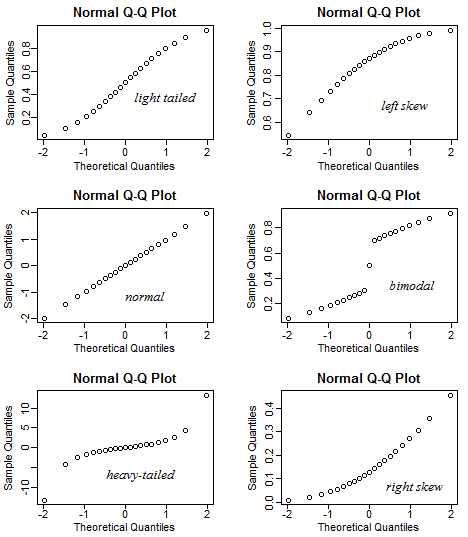
\includegraphics[width=0.6\textwidth]{figures/ch2/qqplot-tutorial}
	\caption{ How information about may be extracted from QQplots. Source: "How to interpret a QQ plot" [Online]. Available: \href{https://stats.stackexchange.com/questions/101274/how-to-interpret-a-qq-plot}{https://stats.stackexchange.com/questions/101274/how-to-interpret-a-qq-plot} [Accessed 09 June 2017]}
	\label{fig:qqplot-tutorial}
\end{figure*}


Another way to analyze scalling characteristics is through QQplots. QQplot is a visual method to compare sample data with a specific stochastic distribution. It orders the sample data values from the smallest to largest, then plots it against the expected value given by the probability distribution function. The data sample values appear along the y-axis and the expected values along the x-axis. The more linear, the more the data is likely to be expressed by this specific stochastic distribution.

Dependendin on the type of plot, some behavios of the empirical dataset, compared to the theoretical may be observed. In the figure ~\ref{fig:qqplot-tutorial} is presented a sumary. 




%%%%%%%%%%%%%%%%%%%%%%%%%%%%%%%%%%%%%%%%%%%%%%%%%%%%%%%%%%%%%%%%%%%%%%%%%%%%%%%%
\subsection{QoS/QoE Related Metrics}

For the point of view of a traffic generation, is interesting that the QoS and QoE metrics present similar values to the ones found on real scenarios. As stated by Magyesi and Szabó\cite{validate-trafficgen}, important QoS/QoE metrics on validation of workload tools are: Round trip Time values (RTT), avarage queue whaiting time and queue size. Still on queue size, self-similar traffic consumes router buffers faster than Poisson traffic\cite{multi-player-online-game-self-similarity}.


%%%%%%%%%%%%%%%%%%%%%%%%%%%%%%%%%%%%%%%%%%%%%%%%%%%%%%%%%%%%%%%%%%%%%%%%%%%%%%%%
\subsection{Study cases}

\subsubsection{Swing}
Swing\cite{swing-paper} is at the present time, one of the main references of realistic traffic generation.  The authors extracted bidirectional metrics from a network link of synthetic traces. Their goals were to get  realism, responsiveness, and randomness.  They define realism as a trace that reflects the following characteristics of the original: 

\begin{itemize}
\item Packet inter-arrival rate and burstiness across many time scales;
\item Packet size distributions;
\item Flow characteristics as arrival rate and length distributions;
\item Destination IPs and port distributions.
\end{itemize}

The traffic generator uses a structural model the account interactions between many layers of the network stack. Each layer has many control variables, which is randomly generated by a stochastic process.  They begin the parameterization, classifying tcpdump\cite{web-libpcap} \textit{pcap}  files with the data, they are able to estimate parameters. 

They validate the results using public available traffic traces, from Mawi\cite{web-mawi} and CAIDA\cite{web-caida}. On the paper, the author focuses on these validation metrics:

\begin{itemize}
\item Comparison of estimated parameters of the original and swing  generated traces;
\item Comparison of aggregate and per-application bandwidth and packets per seconds ;
\item QoS metrics such as two-way delay and loss rates;
\item Scaling analysis, via Energy multiresolution energy analysis.
\end{itemize}


To the vast majority of the results, both original and swing traces results were close from each other. Thus,  Swing was able to match aggregate and burstiness metrics, per byte and per packet, across many time scales.  


%%%%%%%%%%%%%%%%%%%%%%%%%%%%%%%%%%%%%%%%%%%%%%%%%%%%%%%%%%%%%%%%%%%%%%%%%%%%%%%%
\subsubsection{Harpoon}

Harpoon\cite{harpoon-validation}\cite{harpoon-paper} is a traffic generator able to generate representative traffic at IP \textit{flow level}. It is able to generate TCP and IP with the same byte, packet, temporal and spatial characteristics measured at routers. Also, Harpoon is a self-configurable tool, since it automatically extracts parameters from network traces. It estimates some parameters from original traffic trace: file sizes, inter-connection times, source and destination IP addresses, and the number of active sessions. 

As proof of concept \cite{ harpoon-validation}, the authors compared statistics from original and harpoon's generated traces. The two main types of comparisons: diurnal throughput, and for stochastic variable CDF and frequency distributions. Diurnal throughput refers to the mean bandwidth variation within a day period.  In a usual network, during the day the bandwidth consumption is larger, and at night smaller. Also, they compared:

\begin{itemize}
\item CDF of bytes transferred per 10 minutes
\item CDF of packets transferred per 10 minutes
\item CDF of inter-connection time
\item CDF of file size
\item CDF of flow arrivals per 1 hour
\item Destination IP address frequency
\end{itemize}

At the end, they showed the differences on throughput evaluation of a Cisco 6509 switch/router using Harpoon and a constant rate traffic generator.  
Harpoon was proven able to give close CDFs, frequency and diurnal throughput plots compared to the original traces. Also, the results demonstrated that Harpoon provide a more variable load on routers, compared to a constant rate traffic. It indicates the importance of using realistic traffic traces on the evaluation of equipment and technologies. 

%%%%%%%%%%%%%%%%%%%%%%%%%%%%%%%%%%%%%%%%%%%%%%%%%%%%%%%%%%%%%%%%%%%%%%%%%%%%%%%%
\subsubsection{D-ITG}

D-ITG\cite{ditg-paper} is a network traffic generator, with many configurable features. The tool provides a platform that meets many emerging requirements for a realistic traffic generation. For example, multi-platform, support of many protocols, distributed operation, sending/receiving flow scalability, generation models, and analytical model based generation high bit/packet rate. You can see different analytical and models and protocols supported by D-ITG at table ~\ref{tab:trafficgen-list1}. 

We will focus on the evaluation of realism on analytical model parameterization.  It is a synthetic replication of a LAN party of eight players of Age of Mythology \footnote{\href{https://www.ageofempires.com/games/aom/}{https://www.ageofempires.com/games/aom/}}. They have captured traffic flows during the party. Then, they modeled its packet size and inter-packet time distributions. They show that the synthetic traffic and the analytical model have similar curves of packet size and inter-packet time, thus it can approximate the empirical data. Also, the mean and the standard deviation of the bit rate of the empirical and synthetic data are similar. 


%%%%%%%%%%%%%%%%%%%%%%%%%%%%%%%%%%%%%%%%%%%%%%%%%%%%%%%%%%%%%%%%%%%%%%%%%%%%%%%%
\subsubsection{sourcesOnOff}


Varet et al. \cite{sourcesonoff-paper} creates an application implemented in C, called SourcesOnOff. It models the activity interval of packet trains using probabilistic distributions. To choose the best stochastic models, the authors have captured traffic traces using TCPdump. Then the developed tool is able to figure out what distribution(Weibull, Pareto, Exponential, Gaussian, etc) fits better the original traffic traces. It uses the Bayesian Information Criterion (BIC) for distance assessment. It tests the smaller BIC for each distribution, and selects it as the best choice. It ensures good correlation between the original and generated traces and self-similarity.

The validation methods used on sourcesOnOff are: 
\begin{itemize}
\item Visual comparison between On time and Off time of the original trace and the stochastic fitting;
\item QQplots, which aim to evaluate the correlation between inter-trains duration of real and generated traffic;
\item Measurement of Autocorrelation\footnote{
The autocorrelation functions measures the correlation between data samples $y_{t}$ and $y_{t + k}$, where $k =0, ..., K$, and the data sample $\{y\}$  is generated by an stochastic process.

According to \cite{book-time-series-analysis}, the autocorrelation for a lag $k$ is:

\begin{equation}
r_{k} = \frac{c_{k}}{c_{0}}
\end{equation}

where 

\begin{equation}
c_{k} = \frac{1}{T - 1}\sum_{t = 1}^{T - k} (y_{t} - \bar{y})(y_{t+k} - \bar{y})
\end{equation}

and $c_{0}$ is the sample variance of the time series. 
} of the measured throughput of the real and synthetic traffic;
\item Hurst exponent computation of the real and the synthetic trace;
\end{itemize}

The results pointed to a good stochastic fitting, but better for On time values. On the other hand, the correlation value of the QQplot was bigger on the Off time values (99.8\% versus 97.9\%). In the real and synthetic traces, the autocorrelation of the throughput remained between an upper limit of 5\%. Finally, the ratio between the evaluated Hurst exponent always remained smaller than 12\%.


%%%%%%%%%%%%%%%%%%%%%%%%%%%%%%%%%%%%%%%%%%%%%%%%%%%%%%%%%%%%%%%%%%%%%%%%%%%%%%%%
\subsubsection{MoonGen}

MoonGen\cite{moongen-paper} is a high-speed scriptable paper capable of sature  10 GnE link with 64 bytes packets, using a single CPU core. The authors have built it over DPDK and LuaJit, enabling the user to have high flexibility on the crafting of each packet, through Lua scripts. It has multi-core support and runs on commodity server hardware. It is able to test latency with sub-microsecond precision and accuracy, using hardware timestamping of modern NICs cards. The Lua scripting API enable the implementation and high customization along with high-speed. This includes the controlling of packet sizes and control of inter-departure times.

The authors evaluated this traffic generator focused on throughput metrics, rather than others. Also, they have small packet sizes (64 bytes to 256), since the per-packet costs dominate. In their work, they were able to surpass 15 Gbit/s with an XL710 40 GbE NIC. Also, they achieve throughput values close to the line rate with packets of 128 bytes, and 2 CPU cores. 


%%%%%%%%%%%%%%%%%%%%%%%%%%%%%%%%%%%%%%%%%%%%%%%%%%%%%%%%%%%%%%%%%%%%%%%%%%%%%%%%
\subsubsection{LegoTG}

Bartlett et al.\cite{legotg-paper} implements a modular framework for composing custom traffic generation, called LegoTG. As argued by the authors (and by this present work), automation of many aspects of traffic generation is a desirable feature. The process of how to generate a proper background traffic may become a research by itself. Traffic generators available today offer a single model and a restricted set of features into a single code base, makes customization difficult. 

The main purpose of their experiment is to show how LegoTG is able to generate background traffic, in a simple way. Also, it shows how a realistic background traffic can influence on research conclusions. The experiment chosen is one of the use cases proposed for Swing\cite{background-traffic-matter}, and its evaluate the error on bandwidth estimation of different measurement tools. It shows that LegoTG is able eble to provide easy and custrom traffic generation.




%%%%%%%%%%%%%%%%%%%%%%%%%%%%%%%%%%%%%%%%%%%%%%%%%%%%%%%%%%%%%%%%%%%%%%%%%%%%%%%%
%\section{An short overview of some Network emerging scenarios}

%\textcolor{red}{TODO}

%%%%%%%%%%%%%%%%%%%%%%%%%%%%%%%%%%%%%%%%%%%%%%%%%%%%%%%%%%%%%%%%%%%%%%%%%%%%%%%%
%\subsection{SDN: Software Defined Networks}

%\textcolor{red}{TODO}

%%%%%%%%%%%%%%%%%%%%%%%%%%%%%%%%%%%%%%%%%%%%%%%%%%%%%%%%%%%%%%%%%%%%%%%%%%%%%%%%
%\subsection{NFV: Network Function Virtualization}

%\textcolor{red}{TODO}

%For NFV instrumentation and benchmark, there are still few works aiming this gap. \cite{instrumentation-framework-nfv} create a web-based framework for NFV instrumentation in bare-metal and embedded level, but the source code is not provided. \cite{nfv-benchmarking-fault} implement some usage cases of NFVIs (Network Function Virtualization Infrastructures) based on fault injection. \cite{nfpa-paper} implement an open-source tool, called NFPA, focusing on benchmarking of Network Functions. 

%%%%%%%%%%%%%%%%%%%%%%%%%%%%%%%%%%%%%%%%%%%%%%%%%%%%%%%%%%%%%%%%%%%%%%%%%%%%%%%%
\chapter{System architecture and Methods}\label{ch:architecture}
%%%%%%%%%%%%%%%%%%%%%%%%%%%%%%%%%%%%%%%%%%%%%%%%%%%%%%%%%%%%%%%%%%%%%%%%%%%%%%%%

% ok1

In this chapter, we will present our tool which aims to fill the gaps addressed in the chapter ~\ref{ch:introduction}. It is called SIMITAR (SnIffing, ModellIng and TrAffic geneRation) and aims to generate a platform-agnostic traffic: it can use as traffic generator engine almost any traffic generator tools and programming API. It just requires a programming or command line interface. SIMITAR creates a  model in XML based on actual traces (\textit{pcaps} or real-time captures), we call Compact Trace Descriptor (CTD). 


We abstract its whole operation cycle in the figure ~\ref{fig:cycle-of-operation}. Our tool, from live captures or \textit{pcap} file collects raw data from Ethernet traffic. It then breaks these data into different flows and uses this data to generate a set of parameters for our traffic model, using a set of algorithms. Finally, SIMITAR provides these parameters to a traffic generator engine and controls its packets injection.

% cycle of operation
\begin{figure*}[ht!]
        \centering
        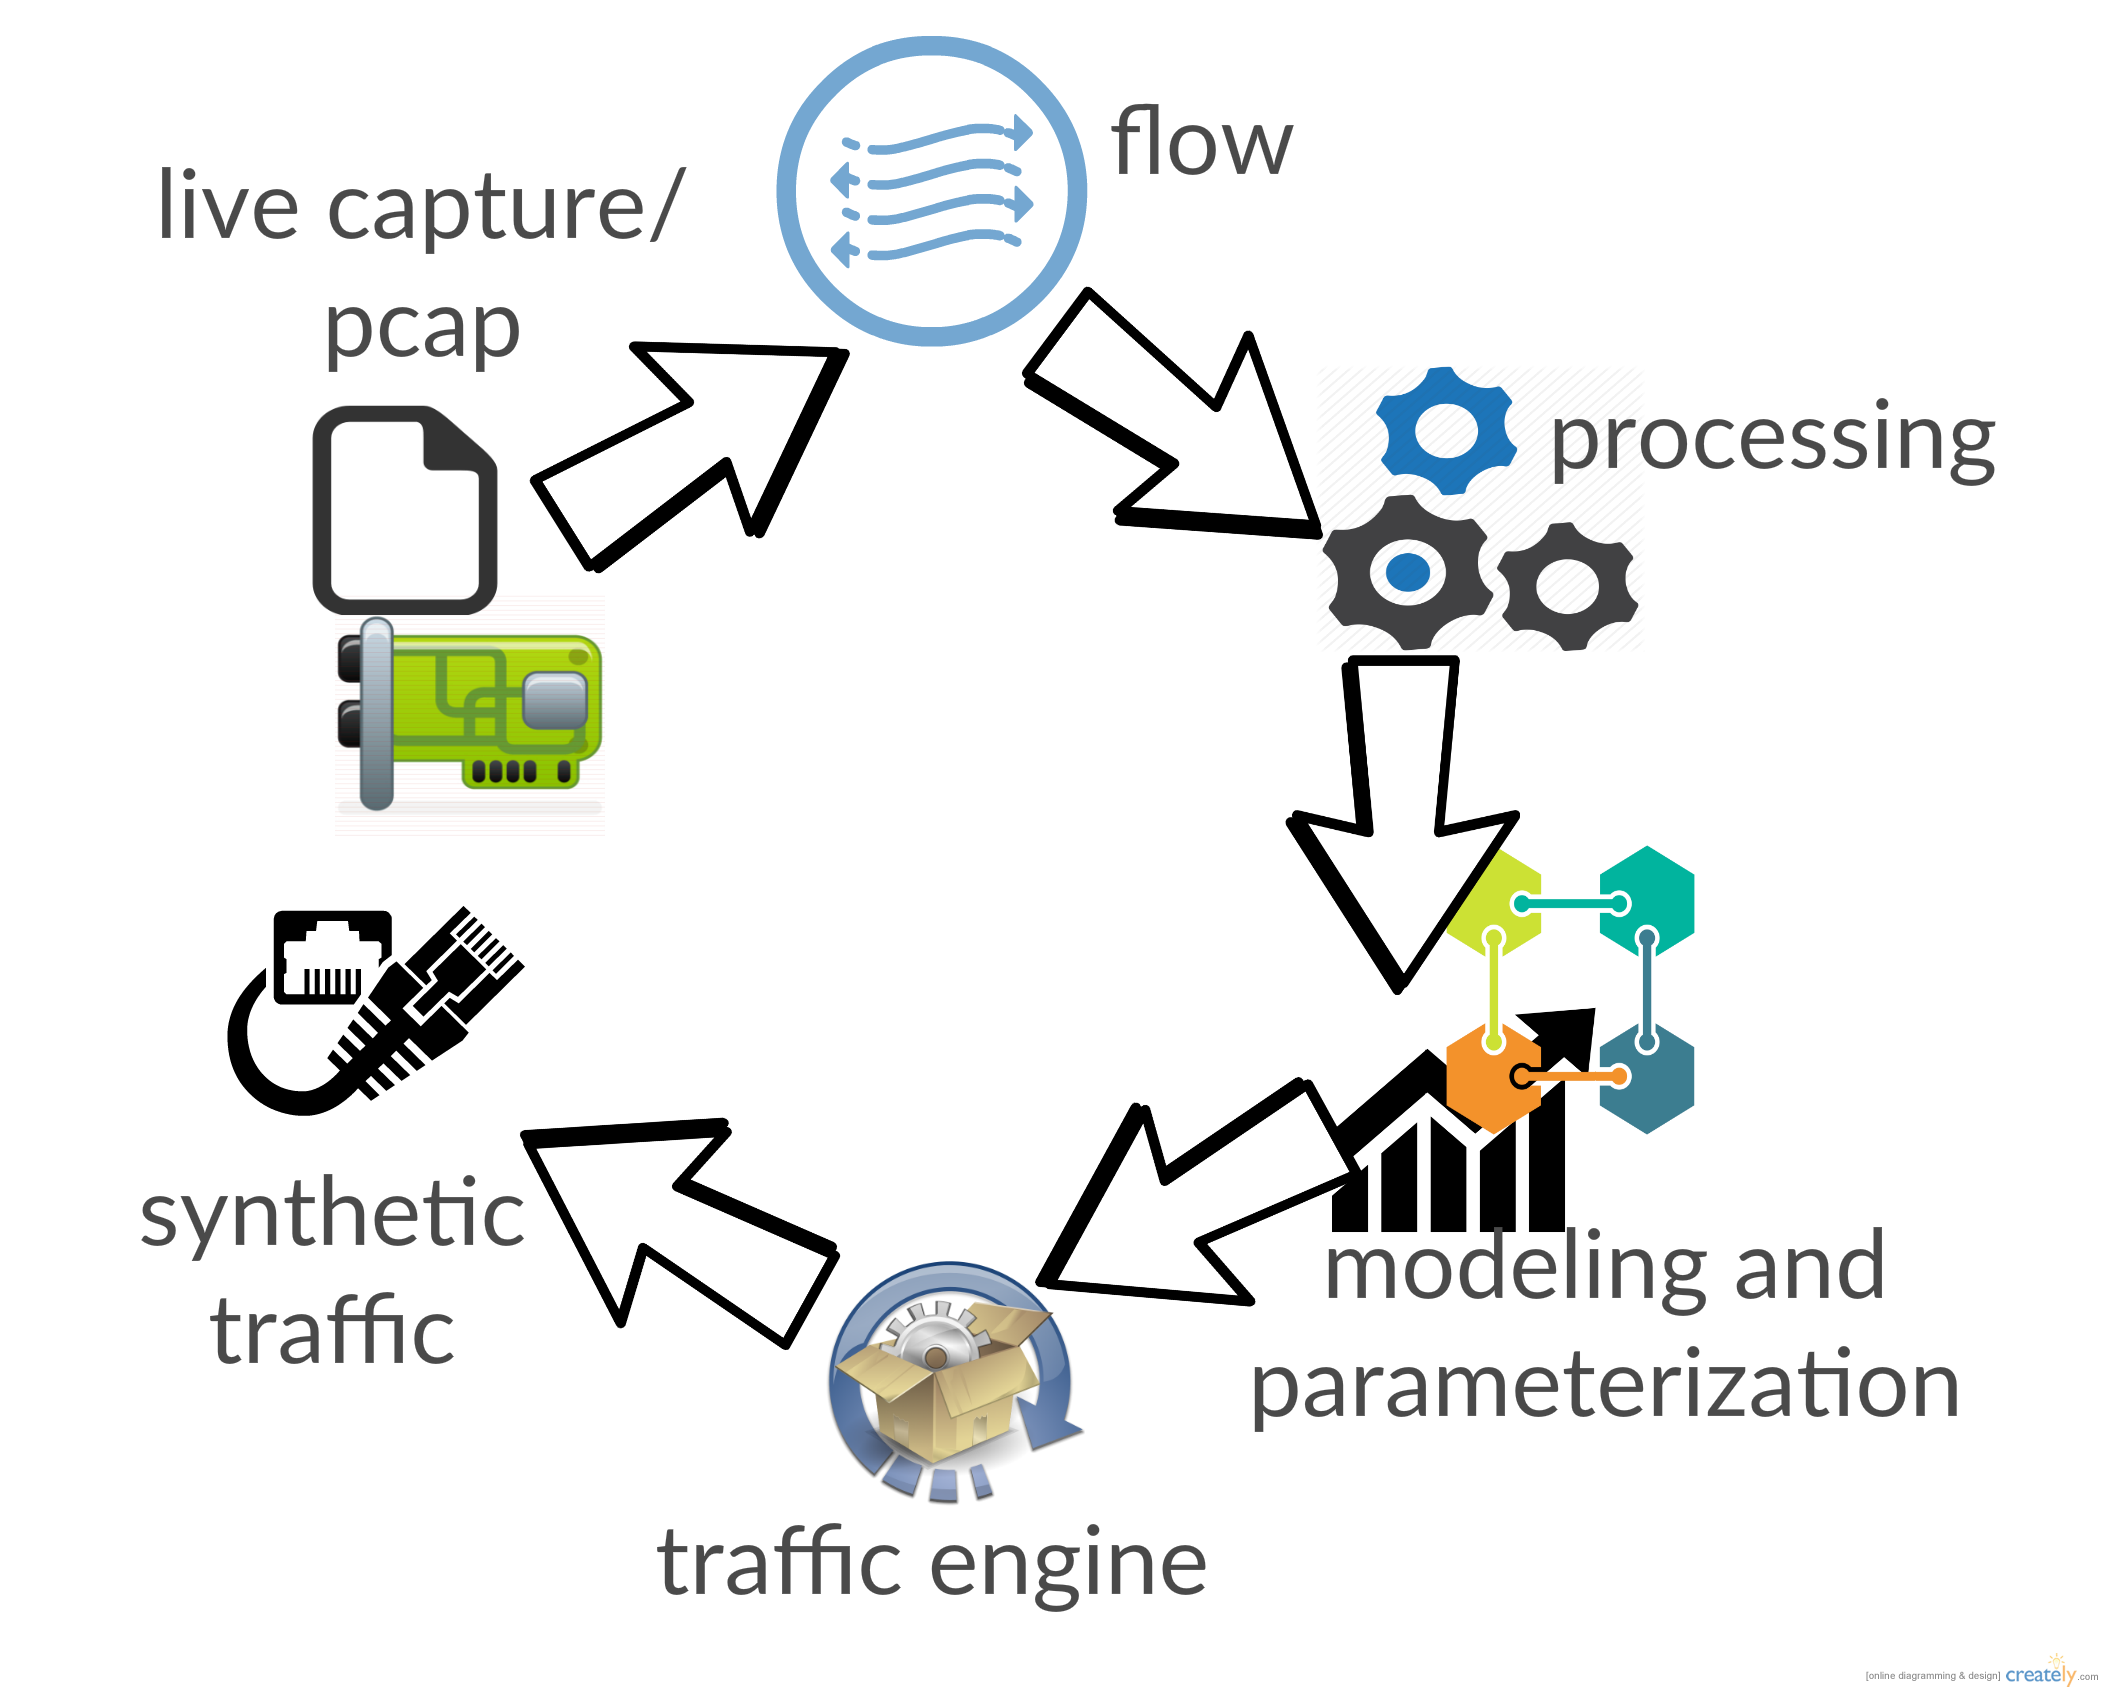
\includegraphics[height=3.0in]{figures/ch3/digram-project-cycle}
        \caption{This figure represents an operation cycle of SIMITAR, emphasizing each main step: sniffing, flow classification, data storing, data processing and fitting, model parameterization,  and synthetic traffic generation.}
    \label{fig:cycle-of-operation}
\end{figure*}


\section{SIMITAR Architecture}

% ok1

To meet the requirements presented in the chapter ~\ref{ch:introduction}, we will define our solution, and how it works. SIMITAR architecture is presented in the figure~\ref{fig:architecture}. It is composed of four components: a \textit{Sniffer}, a \textit{SQLite database}, a \textit{TraceAnalyzer}, a \textit{FlowGenerator};  and a \textit{Network Traffic Generator}, as subsystem. We describe each part below.

% component diagram and module design
\begin{figure*}[ht!]
        \centering
        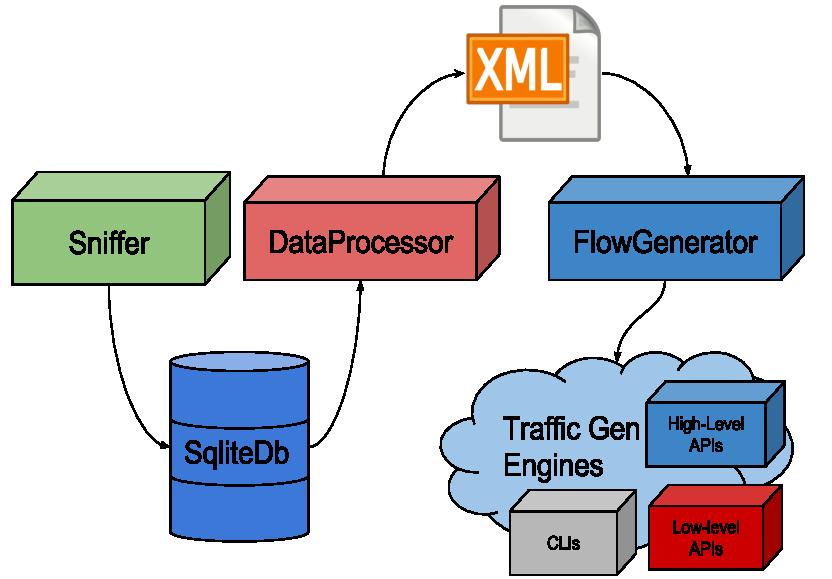
\includegraphics[height=2.7in]{figures/ch3/architecture-diagram}
        \caption{Architecture of SIMITAR}
    \label{fig:architecture}
\end{figure*}


%%%%%%%%%%%%%%%%%%%%%%%%%%%%%%%%%%%%%%%%%%%%%%%%%%%%%%%%%%%%%%%%%%%%%%%%%%%%%%%%
\subsection{Sniffer}

% ok1

This component collects network traffic data and classifies it into flows, storing stores in an SQLite database. It defines each flow by the same criteria used by SDN switches\cite{sdn-survey},  through header fields matches. It uses:

\begin{itemize}
\item Link Protocol
\item Network Protocol
\item Network Source and Destination Address
\item Transport Protocol
\item Transport Source and Destination Port
\end{itemize}

\begin{figure*}[ht!]
        \centering
        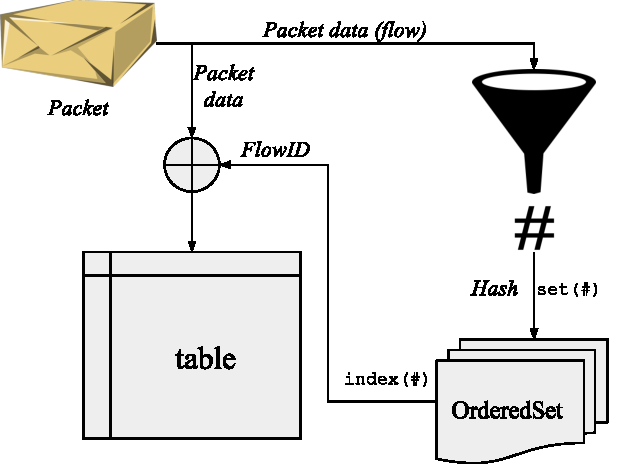
\includegraphics[height=2.5in]{figures/ch3/sniffer-classifier}
        \caption{SIMITAR's sniffer hash-based flow classification}
    \label{fig:sniffer}
\end{figure*}


We implemented the first version of this component in Shell Script (Bash).  Tsahrk\footnote{\href{https://www.wireshark.org/docs/man-pages/tshark.html}{https://www.wireshark.org/docs/man-pages/tshark.html}} was used to extract header fields, and Awk to match the flows, and Sed/Awk to create the SQLite queries. This version was too slow to operate in real time on Ethernet interfaces. On the other hand, this approach was fast to implement and enable the implementation of the other components. The second and current version was made using Python. This version used Pyshark \footnote{\href{https://pypi.python.org/pypi/pyshark}{https://pypi.python.org/pypi/pyshark}} as sniffer library.  


It has a data structure we developed called \textit{OrderedSet}. A set is a list of elements with no repetition but does not keep track of the insertion order. Our OrderedSet does. Also, it makes use of a  64 bits hash function of the family FNV\footnote{The collision probability of a good 64 bits hash function in a table with 10000 items is about of $2.71e-12$.}. The listed header fields are inputs for a hash function, and its value is set on the ordered set which returns its order (index on the \textit{OrderedSet}). The index value is chosen as a packet flowID.  


%c++ http://ideone.com/F0V42m
As future improvements for this component, we propose a more efficient implementation in C++ and data visualization for the collected data. In that way, we may optimize the packet processing. We discuss this in deeper details in the chapter~\ref{ch:conclusion}.


%%%%%%%%%%%%%%%%%%%%%%%%%%%%%%%%%%%%%%%%%%%%%%%%%%%%%%%%%%%%%%%%%%%%%%%%%%%%%%%%
\subsection{SQLite database}

\begin{figure*}[ht!]
        \centering
        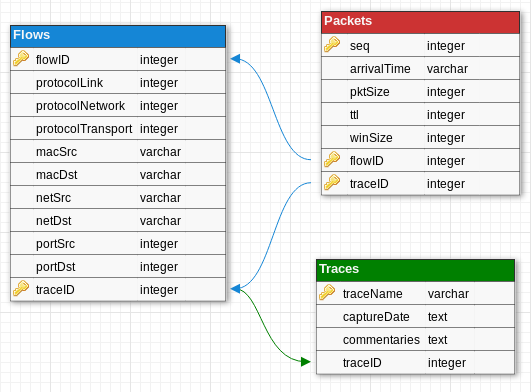
\includegraphics[height=3.0in]{figures/ch3/database-relational-model}
        \caption{SIMITAR's SQLite database relational model}
    \label{fig:simitar-database}
\end{figure*}

% ok1

The database stores the collected raw data from the traces for further analysis. The \textit{Sniffer} and the \textit{TraceAnalyzer} components uses the database.  We choose an SQLite database, because according to its specifications\footnote{\href{https://www.sqlite.org/whentouse.html}{https://www.sqlite.org/whentouse.html}}, it fits well our purposes. It is simple and well-suitable for an amount of data smaller than terabytes. In the figure ~\ref{fig:simitar-database} we present the relational model of our database, which stores a set of features extracted from packets, along with the flowID calculated by the sniffer component. 


\subsection{Trace Analyzer}

% ok1

This module is the core of our project. It creates a trace model via the analysis of the collected data. We define here a Compact Trace Descriptor (CTD) as a human and machine-readable file, which describes a traffic trace through a set of flows, each of them represented by a set of parameters, such as header information and analytical models.  The Trace Analyze has the task to learn these features from raw traces data (stored in the SQLite database) and generate an XML file.  In the figure~\ref{fig:CTD-diagram} we show a directory diagram of a CDT file. It has many of many flow fields, and each one contains each parameter estimated. Now we will describe how we construct it. 


\begin{figure}
\centering
\subfloat[first]{
  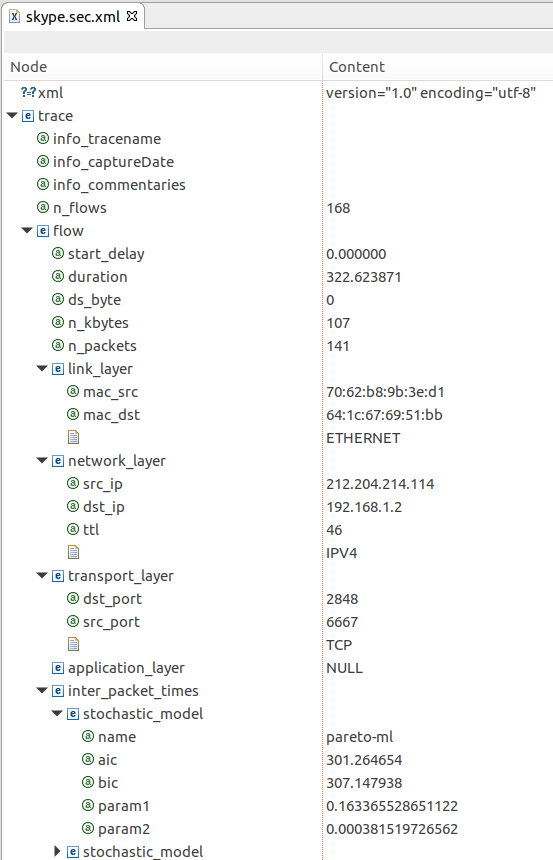
\includegraphics[height=4.in]{figures/ch3/cdt1}
}
\subfloat[second]{
  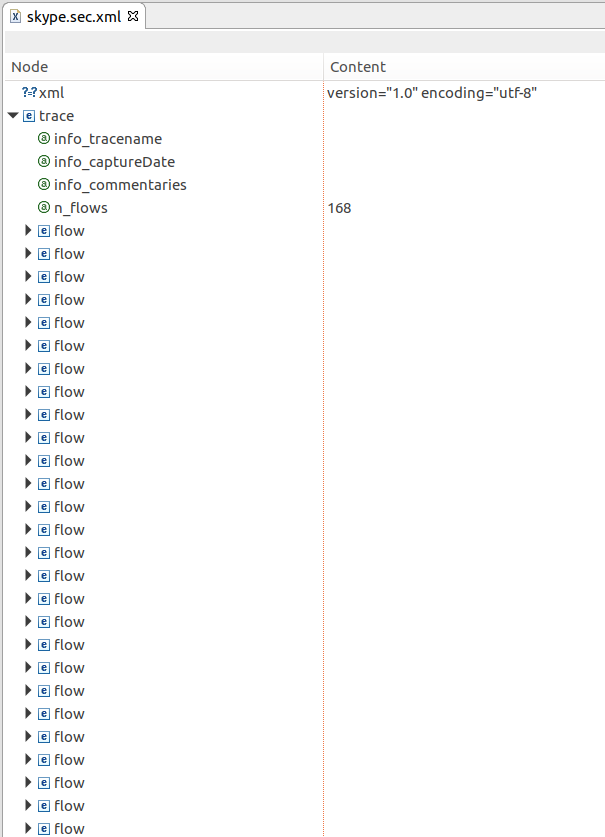
\includegraphics[height=4.in]{figures/ch3/cdt2}
}
\caption{Directory diagram of the schema of a Compact Trace Descriptor (CDT) file. On the left, we present a dissected flow, and on the right a set of flows.}
\label{fig:CTD-diagram}
\end{figure}


\subsubsection{Flow features}

% ok1 

Some unique per-flow features are directly measured from the data. They are:  

\begin{itemize}
\item Flow-level properties like duration of flow, start delay, number of packets per flow, number of KBytes per flow; 
\item Header fields, like protocols, QoS fields, ports, and addresses.
\end{itemize}

Each one of these parameters is unique per flow. Other features like PSD (packet size distribution) e IPT (Inter-packet time), have a more complex behavior.  To represent these characteristics, we will use sets of stochastic-based models.  


\subsubsection{Inter Packet Times}

\begin{figure*}[ht!]
    \centering
    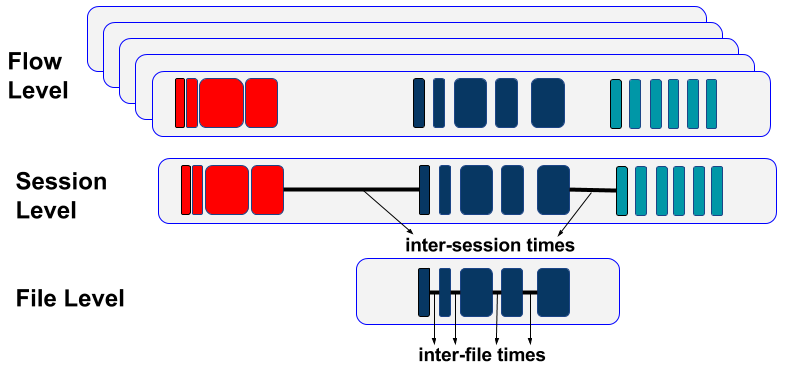
\includegraphics[height=2.0in]{figures/ch3/modified-harpoon-model}
    \caption{The schema of the modified version of the Harpoon algorithm we adopt on SCIMITAR.}
    \label{fig:modified-harpoon-model}
\end{figure*}


To represent inter-packet times, we adopt a simplified version of the Harpoon's traffic model. A deep explanation of the original model can be found at \cite{harpoon-paper} and \cite{harpoon-validation}. Here, we will explain our simplified version, which is illustrated at figure~\ref{fig:modified-harpoon-model}. 


Harpoon uses a definition of each level, based on the measurement of SYN and ACK TCP flags. It uses TCP flags (SYN) to classify packets in different levels, named their file, session, and user level. We choose to estimate these values, based on inter-packet times only. The distinction is made based on the time delay between packets.


In our algorithm simplified version, we define three different layers of data transference to model and control: file, session, and flow. For SIMITAR, a file is just a sequence of consecutive packets transmitted continuously, without large interruption of traffic. It can be, for example, packets sent downloading a file, packets from a  UDP  connection or a single ICMP echo packet. The session-layer refers to a sequence of multiple files transmitted between a source and a destination, belonging to the same flow.  The flow level refers to the conjunct of flows, as classified by the Sniffer.  Now, we explain SIMITAR operation on each layer. 


In the \textbf{flow layer} the \textit{TraceAnalyzer} loads the flow arrival times from the database and calculates the inter-packet times within the flow context. 


At the \textbf{session layer}, we use a deterministic approach for evaluating file transference time and times between files: ON/OFF times sequence of packet trains. We choose a deterministic model because in this way we can express diurnal behavior\cite{harpoon-paper}.  We develop an algorithm called \textit{calcOnOff} responsible for estimating these times. It also determines the number of packets and bytes transferred by each file. Since the ON times will serve as input for actual traffic generators, we defined a minimum acceptable time for on periods equals to 100 ms. ON times can be arbitrary smalls, and they could be incompatible with acceptable ON periods for traffic generators. Also in the case of just one packet, the ON time would be zero. So setting a minimum acceptable time to solve these issues. The OFF times, on the other hand, are defined by the constant \texttt{session\_cut\_time} \footnote{In the code it is called \texttt{DataProcessor::m\_session\_cut\_time} }. If the time between two packets of the same flow is larger than \texttt{session\_cut\_time}, we consider them belonging to a different file, so this time is a session OFF time. In this case, we use the same value of the constant \textit{Request and Response timeout} of Swing\cite{swing-paper} for the \texttt{session\_cut\_time}: 30 seconds. The control of ON/OFF periods in the traffic generation is made by the \textit{Flow Generator} component \footnote{This control is made by the class \texttt{NetworkFlow}}.


In the \textbf{file layer}, we model the inter-packet times at the file level. To estimate inter-packet times within files, we select all inter-packet times smaller than \texttt{session\_cut\_time}\footnote{In the code it is called\texttt{DataProcessor::m\_session\_cut\_time} }. All files within the same flow are considered to follow the same model. We delegate the control of the inter-packet times to the underlying workload engine tool. We ordered them, from the best to the worst. Currently, we are using eight different stochastic functions parameterizations. They are Weibull(linear regression), Normal(mean/standard deviation calculation), Exponential(mean and linear regression estimation), Pareto(linear regression and maximum likelihood), Cauchy(linear regression) and Constant(mean calculation). From those, Weibull, Pareto, and Cauchy are heavy-tailed functions, and therefore self-similar processes. But if the flow has less than 30 packets, just the constant model is evaluated. It is because numerical methods gave poor results if the data sample used is small. We sort these models according to the Akaike Information Criterion (AIC) as default\cite{sourcesonoff-paper}\cite{bic-aic-comparision}. We will enter into deeper details on this methodology on the chapter ~\ref{ch:modeling-evaluation}. The methodology of selection is presented in the figure~\ref{fig:model-parameterization}, and all constants and modes of operation can be changed by command line options.


\begin{figure*}[ht!]
    \centering
    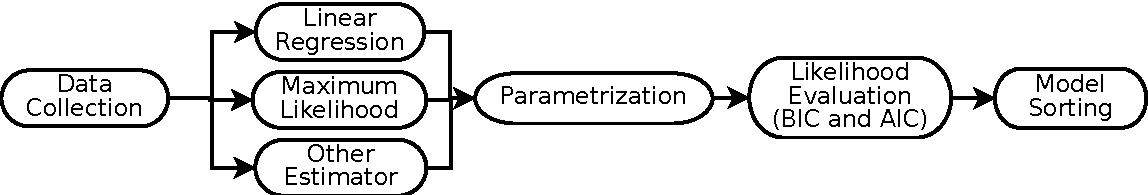
\includegraphics[height=0.9in]{figures/ch3/simitar-parametrization}
    \caption{Diagram of parameterization and model selection for inter-packet times and inter-file times.}
    \label{fig:model-parameterization}
\end{figure*}


\subsubsection{Packet Sizes}



Our approach for the packet size is much simpler. Since the majority of packet size distribution found on real measurements are bi-modal \cite{packet-distribution-model}\cite{sourcesonoff-paper}\cite{udp-flows-model}, we first sort all packet sizes of flow in two modes. We define a packet size mode cut value of 750 bytes, same value adopted by \cite{udp-flows-model}. 


We know how much packets each mode has, and then we fit a model for it. We use three stochastic models: constant, exponential and normal. Since self-similarity does not make sense for packet-sizes, we prefer to use just the simpler models. When there is no packet for a model, we set a flag NO\_MODEL, and when there is just a single packet we just use the constant model. Then calculate the BIC and AIC for each, but we decide to set the constant model as the first.

As is possible to see in many works \cite{packet-distribution-model} \cite{udp-flows-model}, since the standard deviation of each mode tends to be small, constant fittings use to give good approximations. Also, it is computationally cheaper for the traffic generated than the other models, since no calculation is a need for each packet sent. Since both AIC and BIC criteria always will select the constant model as the worst, we decide to ignore this.


\subsubsection{Compact Trace Descriptor}

%2nd-review
An example of the final result of all the methods is presented in the XML code down below. It illustrates a flow of a \textit{Compact Trace Descriptor}(CDT) file. The traffic models for inter-packet times are grouped by the tag \texttt{inter\_packet\_times}, and the packet trains by the tag \texttt{session\_times}. All the times are in seconds, and \texttt{inf} represents infinity. The protocol of each layer is stored as data by each tag.

\begin{minted}[frame=single,
               framesep=3mm,
               linenos=true,
               xleftmargin=21pt,
               tabsize=4,
               fontsize=\scriptsize, 
               breaklines=true]{xml}
               
	<flow start_delay="0.144400" duration="317.744333" ds_byte="0" n_kbytes="40" n_packets="344">
		<link_layer mac_src="64:1c:67:69:51:bb" mac_dst="70:62:b8:9b:3e:d1">ETHERNET</link_layer>
		<network_layer src_ip="192.168.1.1" dst_ip="192.168.1.2" ttl="64">IPV4</network_layer>
		<transport_layer dst_port="2128" src_port="53">UDP</transport_layer>
		<application_layer>DNS</application_layer>
		<inter_packet_times>
			<stochastic_model name="pareto-ml" aic="-1165.310696" bic="-1157.646931" param1="0.405085202535192" param2="0.002272655895996"/>
			<stochastic_model name="pareto-lr" aic="-454.049749" bic="-446.385984" param1="0.061065000000000" param2="0.002272655895996"/>
			<stochastic_model name="weibull" aic="-246.882037" bic="-239.218273" param1="0.120355000000000" param2="0.001629000000000"/>
			<stochastic_model name="exponential-me" aic="486.370061" bic="494.033826" param1="1.340057495455104" param2="0.000000000000000"/>
			<stochastic_model name="normal" aic="1629.370900" bic="1637.034665" param1="0.746236637899171" param2="2.626808289821357"/>
			<stochastic_model name="exponential-lr" aic="3166.816047" bic="3174.479812" param1="0.009752000000000" param2="0.000000000000000"/>
			<stochastic_model name="cauchy" aic="31737.418442" bic="31745.082207" param1="0.000000000000194" param2="-3152.827055696396656"/>
			<stochastic_model name="constant" aic="inf" bic="inf" param1="0.746236637899171" param2="0.000000000000000"/>
		</inter_packet_times>
		<session_times on_times="29.22199798,73.40390396,151.84077454" off_times="30.85738373,32.42027283" n_packets="19,103,222" n_bytes="2272,12399,26689"/>
		<packet_sizes n_packets="344" n_kbytes="40">
			<ps_mode1 n_packets="344" n_kbytes="40">
				<stochastic_model name="constant" aic="inf" bic="inf" param1="120.232558" param2="0.000000"/>
				<stochastic_model name="normal" aic="2926.106952" bic="2933.788235" param1="120.232558" param2="16.941453"/>
				<stochastic_model name="exponential-me" aic="3987.126362" bic="3994.807645" param1="0.008317" param2="0.000000"/>
			</ps_mode1>
			<ps_mode2 n_packets="0" n_kbytes="0">
				<stochastic_model name="no-model-selected" aic="inf" bic="inf" param1="0.000000" param2="0.000000"/>
			</ps_mode2>
		</packet_sizes>
	</flow>
	
\end{minted}

%2nd-review
%The current version of our tool, do not intrinsically supports responsiveness. The underlying traffic generator API can support it (such as Seagull\cite{web-seagull}), but we do not generate any mathematical model for this purpose, and this may also stand as a future work we discuss on chapter ~\ref{ch:conclusion}. 

\subsection{Flow Generator}

\begin{figure*}[ht!]
    \centering
    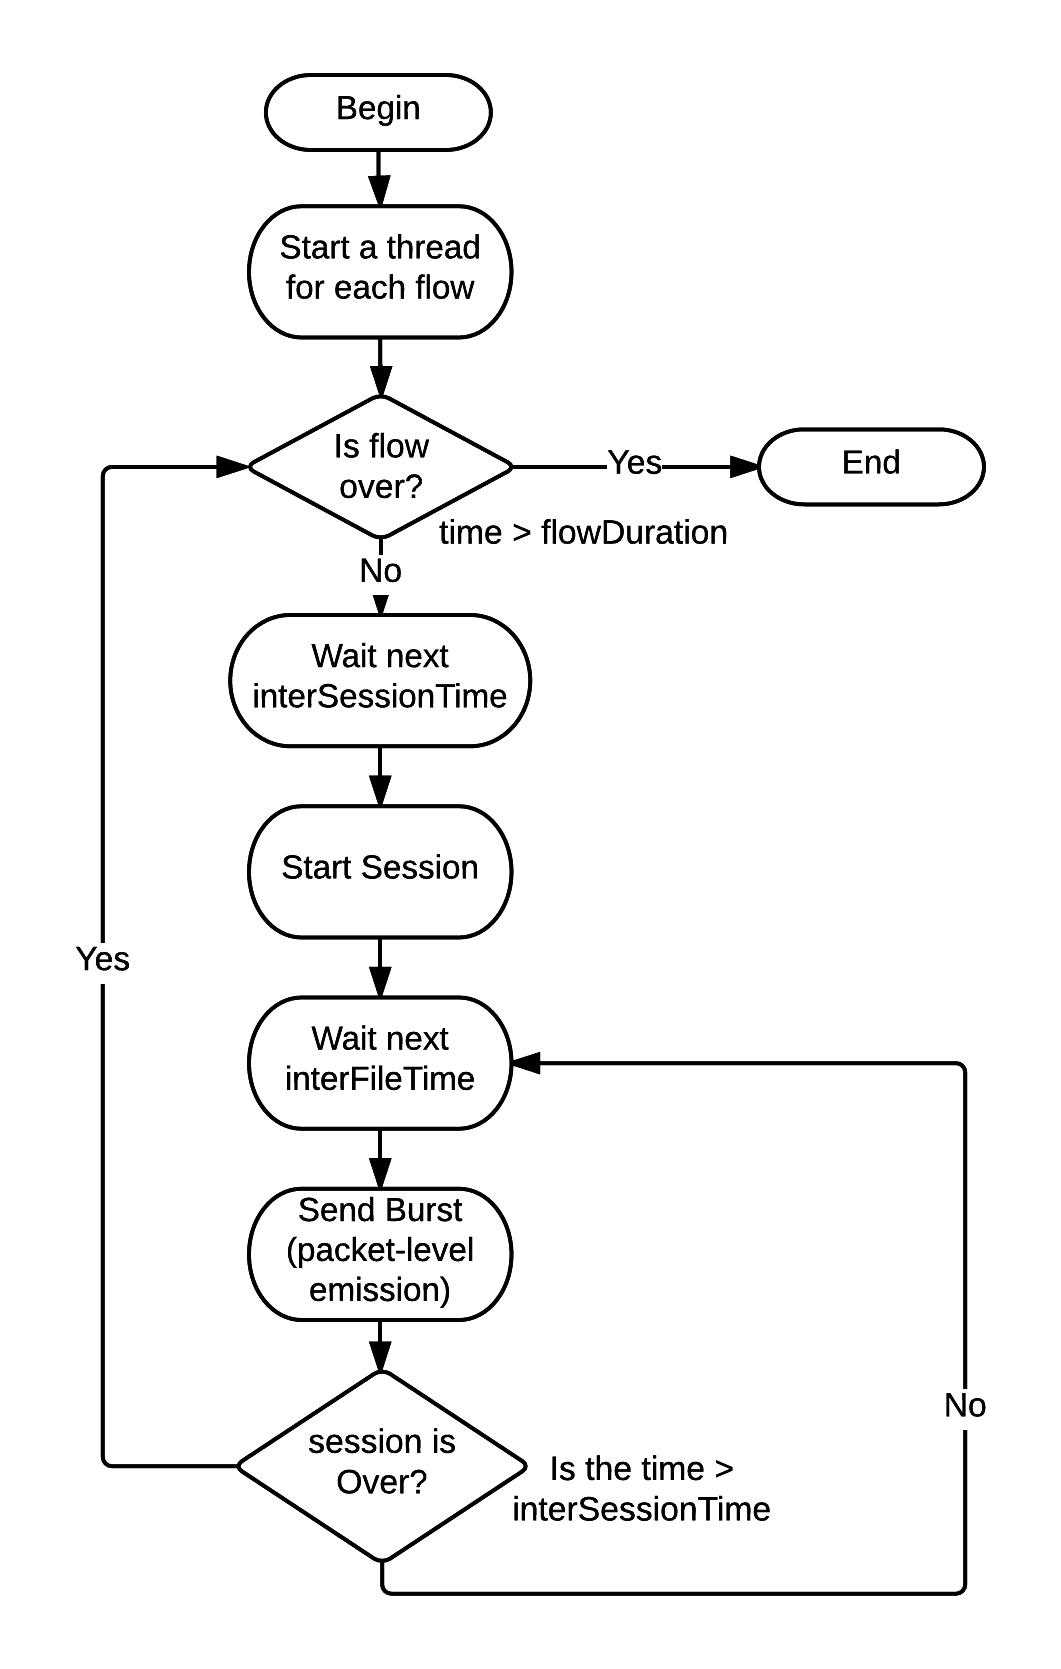
\includegraphics[height=4.5in]{figures/ch3/alg-simplified-harpoon}
    \caption{Simplified-harpoon emission algorithm}
    \label{fig:alg-simplified-harpoon}
\end{figure*}

The Flow Generator handles the data on the CTD file, and use to retrieve parameters for traffic generation. It crafts and controls each flow in a separated thread. 


We first implemented it using the D-ITG API. But our Flow Generator can use any traffic generator with API, CLI or script interface as well. To easily expand this component, we use the design pattern factory. If the user wants to introduce support for a new traffic generator, he just has to expand the class \texttt{DummyFlow} and add the support on the method \texttt{make\_flow()} of the class \texttt{NetworkFlow}. We will discuss this deeper in the next section.


This component works in two different layers according to the traffic generators classification introduced in the chapter ~\ref{ch:literature-review}: at the Flow level, and packet level, as presented in the figure ~\ref{fig:layers-workload-tools}. 

\begin{figure*}[ht!]
    \centering
    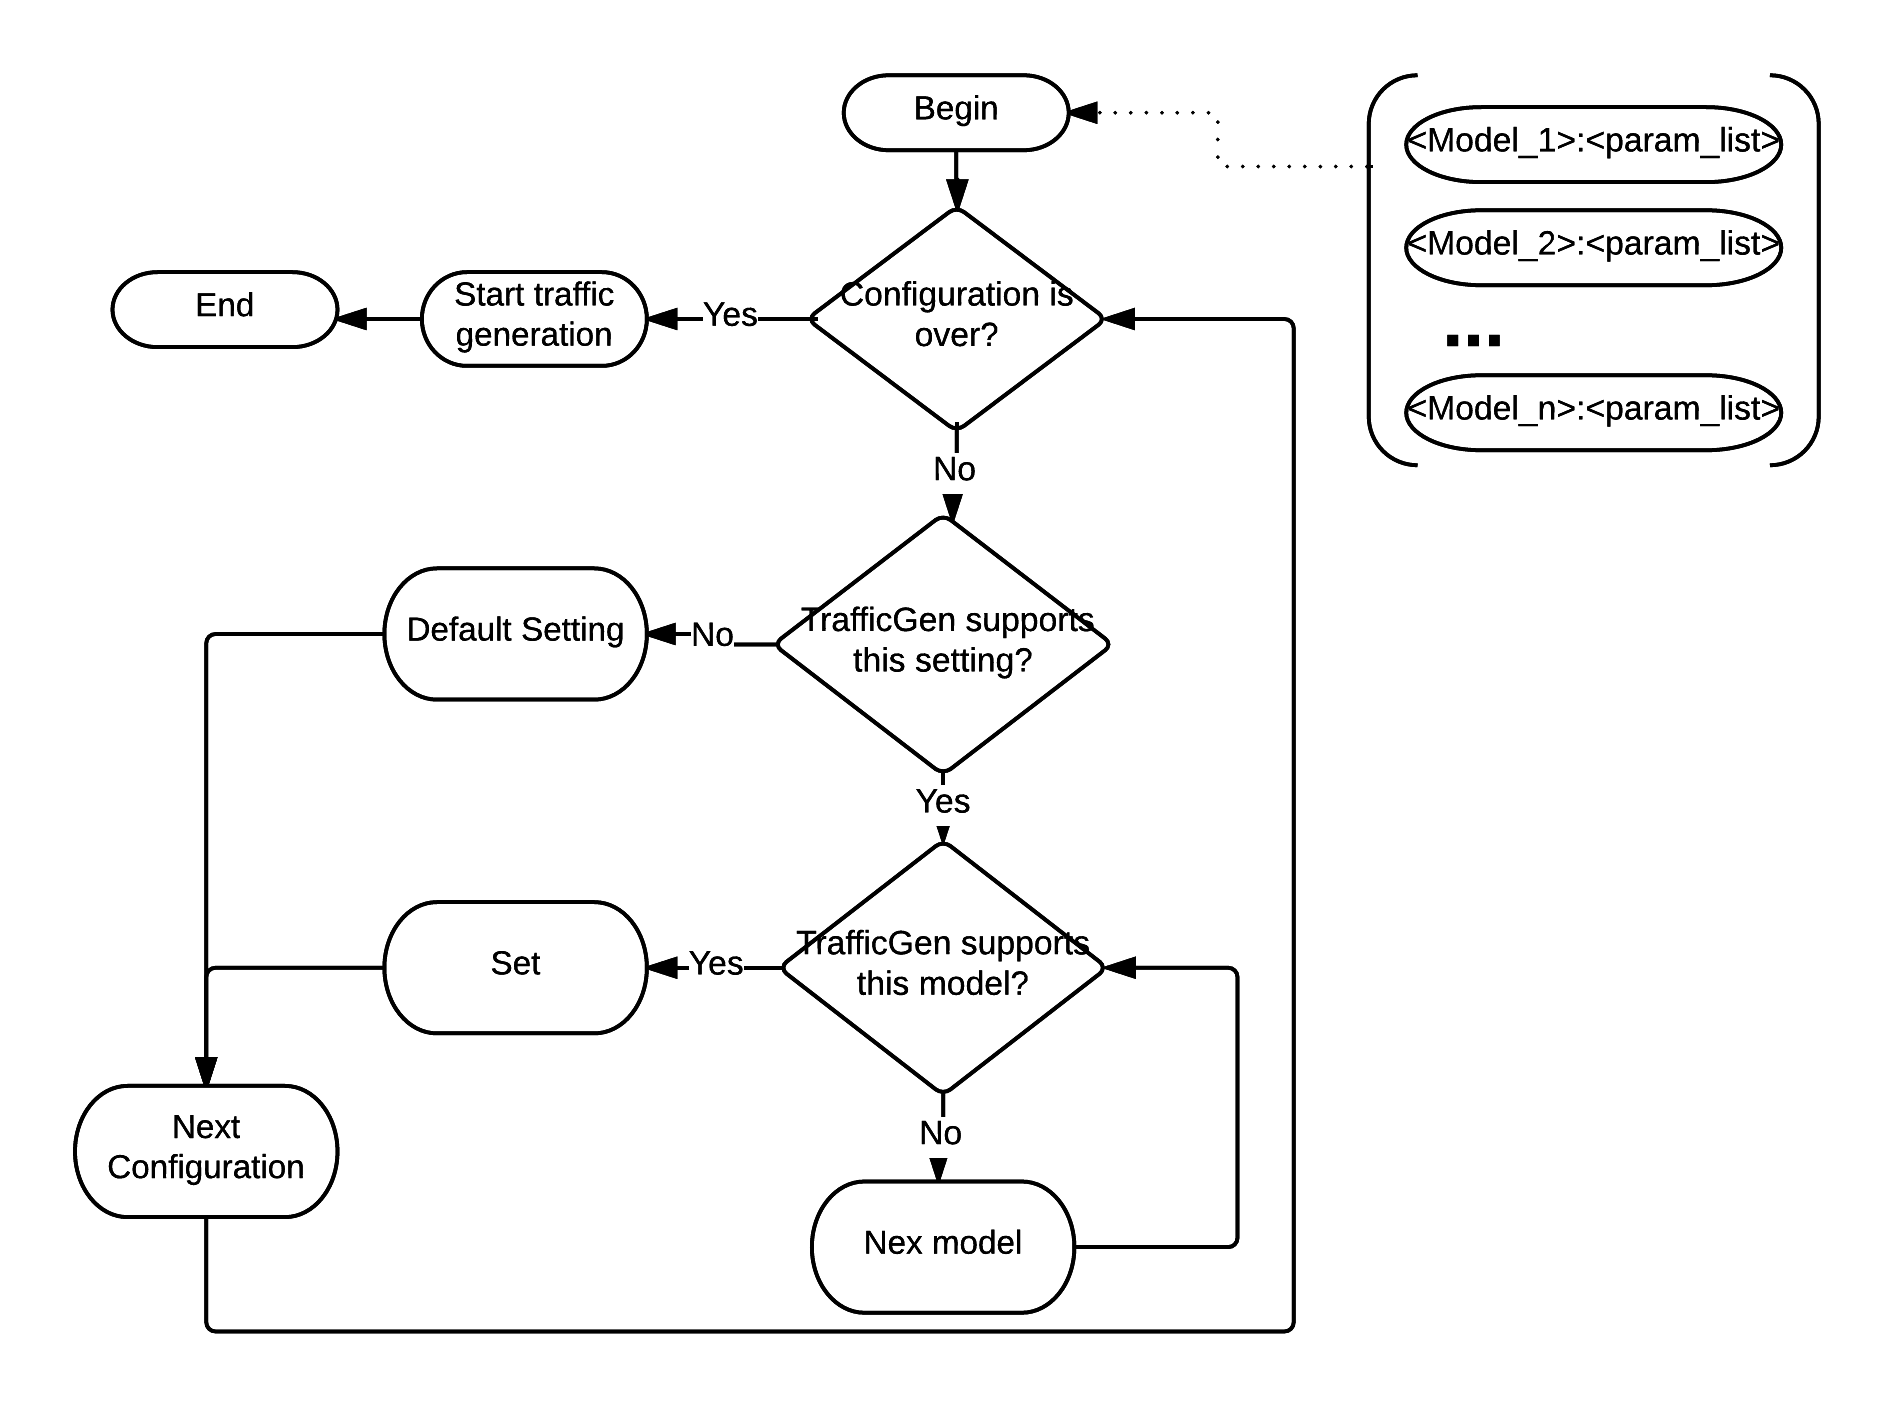
\includegraphics[height=4.0in]{figures/ch3/alg-traffic-engine-config}
    \caption{Traffic engine configuration model}
    \label{fig:alg-traffic-engine-config}
\end{figure*}

\subsubsection{Flow-level Traffic Generation Operation}

At the flow-level, it controls each flow using the algorithm at figure~\ref{alg-simplified-harpoon}. This algorithm handles our model defined at the figure~\ref{fig:modified-harpoon-model}.

%2nd-review
It starts a \textit{thread} for each flow in the \textit{Compact Trace Descriptor}, then the thread sleeps its \texttt{start\_delay}. It is the time when the first flow packet was captured in the original capture. It then calls the underlying traffic generation method, passing to it the file ON time, number of packets and number of bytes to be sent (file size). Then it sleeps the next session OFF time from the stack until it ends. When the list of ON/OFF times is over, the thread ends. 


\subsubsection{Flow Generation Programming}

%2nd-review
At the packet level, it must use the expanded class of the \texttt{DummyFlow}. In this level, the job of our tool is to configure the underlying engine, to send a file, as defined before. Therefore it uses the \textit{getters} available, and the passed parameters, defined by the operation described in the previous session. The implementation of this level should follow the flowchart presented in the figure ~\ref{fig:alg-traffic-engine-config}.
Down below we present a simplistic code of how the D-ITG API can be used to generate packet-level traffic. We call this concept \textit{Flow Generation Programming} A more complex configuration is possible, but it serves to illustrate the procedure. Its API documentation is available at on D-ITG web-site \footnote{\href{http://www.grid.unina.it/software/ITG/manual/index.html\#SECTION00047000000000000000}{http://www.grid.unina.it/software/ITG/manual/index.html\#SECTION00047000000000000000}}. 
\begin{minted}[frame=single,
               framesep=3mm,
               linenos=true,
               xleftmargin=21pt,
               tabsize=4,
               fontsize=\scriptsize, 
               breaklines=true]{c++}
void flowGenerate(const counter& flowId, const time_sec& onTime, const uint& npackets, const uint& nbytes,  const string& netInterface)
{
	char localhost[CHAR_BUFFER];
	string strCommand;
	char command[CHAR_BUFFER];
	uint i = 0;
	int rc = 0;
	getLocalIp("eth0", localhost);
	strCommand += " -t " + std::to_string(onTime); 
	strCommand += " -k " + std::to_string(nbytes / 1024);
	strCommand += " -a " + getHostIP();
	if (this->getTransportProtocol() == PROTOCOL__TCP)
		strCommand += " -T TCP -D ";
	else if (this->getTransportProtocol() == PROTOCOL__UDP)
		strCommand += " -T UDP ";
	else if (this->getTransportProtocol() == PROTOCOL__ICMP)
		strCommand += " -T ICMP ";
	for(;;i++)
	{	
		StochasticModelFit idtModel = this->getInterDepertureTimeModel(i);
		if(idtModel.modelName() == WEIBULL)
		{
			strCommand += " -W " + std::to_string(idtModel.param1()) + " " + std::to_string(idtModel.param2());
			break;
		}
		else if ( idtModel.modelName() == CONSTANT)
		{
			strCommand += " -C " + std::to_string(nbytes/(1024*onTime));
			break;
		}
	}
	strcpy(command, strCommand.c_str());
	rc = DITGsend(localhost, command); // it is not blocking
    usleep(onTime*10e6);
	if (rc != 0)
	{
		printf("\nDITGsend() return value was %d\n", rc);
		exit(EXIT_FAILURE);
	}
}
\end{minted}

\subsection{Network Traffic Generator}


A network traffic generator software that should provide its API or script interface for the \textit{FlowGenerator} component. 
 
Since \texttt{DITGsend()} is thread safe, no mutex is need. It would be needed if a lower level API, such Libtins or Libpcap was used. In that case, these APIs would permit control precisely each packet sent through the interface, but a mutex would be necessary. An scriptable tool, such as Iperf can be used as well, using \texttt{fork()} or \texttt{popen()}.

As we claimed before, this tools is simple of being expanded for almost any traffic generation API, since its modeling framework is not coupled to the traffic generation.
The figure \ref{fig:network-trace-flow-class-diagram} illustrates it well. It presents three possibilities of different traffic generation engines, all being configured and scheduled in a platform-agnostic way.

\begin{figure*}[ht!]
    \centering
    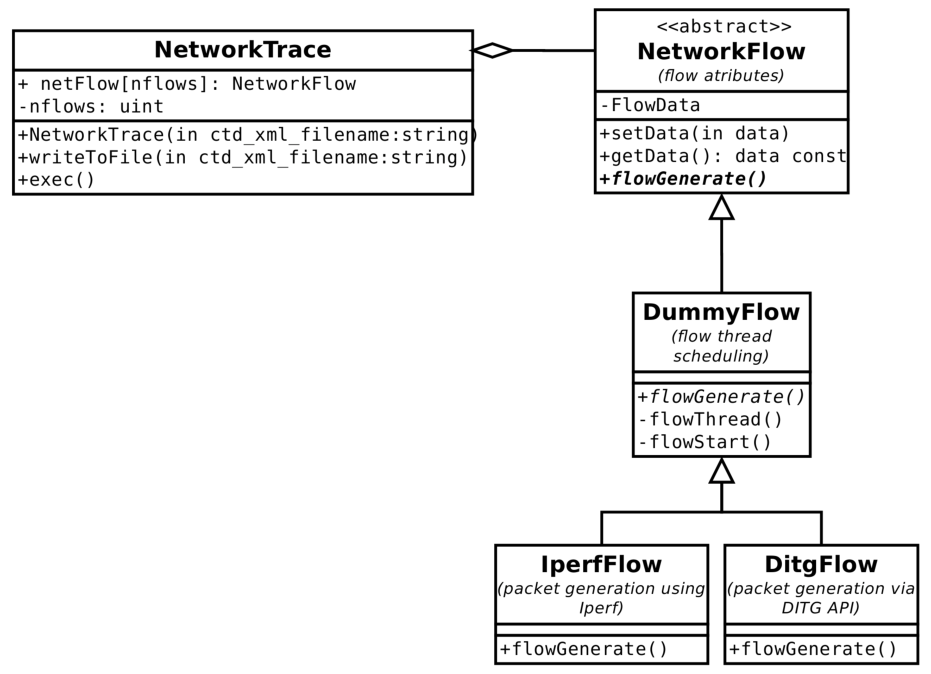
\includegraphics[height=3.0in]{figures/ch3/trace-flow}
    \caption{Class hierarchy of NetworkTrace and NetworkFlow, which enables the abstraction of the traffic generation model of the traffic generation engine.}
    \label{fig:network-trace-flow-class-diagram}
\end{figure*}


\section{Usage and Use Cases}

Each SIMITAR component works as a different application:

\begin{itemize}
	\item \texttt{sniffer-cli.py};
	\item \texttt{trace.db} (sqlite3 database);
	\item \texttt{trace-analyzer}.
	\item \texttt{simitar-gen} (traffic generator).
\end{itemize}


When it working as a sniffer, it strores data from the capture traffic in the sqlite3 database. It may work over a \textit{pcap} file or an Ethernet interface. Working as a trace a trace-analyzer, it receive the name of the trace as stored in the database, and creates a XML compact trace descriptor. The constants used in the modelling may be changed and provided as command line argument. If not, the default values will be used. 

As a traffic generator it may work as a client or a server. Working as a server is necessary for tools that require establishing a connection before generate the traffic, such as Iperf and D-ITG. It will just work passivaly. Working as a client, is acts as a traffic emissor. Tools such as \textit{libtins} dos not require server operation the send the traffic. 

When it operates as a client or as packet injector, it is operating as a traffic generator. The difference is that as a client, the used traffic generator is connection-oriented. It needs to establish a connection with the destination host (the server), before start sending packets. Operating as a client, it must take as an input a list of IP or MAC destination addresses, since they will not match with the ones in the original trace. It takes as an input a single destination in the command line, or list of many, in a text file passes as a parameter. Also, it uses the machine IP address as packet's source IP.

 As a packet injector can generate packets on the output interface, without establishing a connection. It uses the original IP and MAC destination and source addresses. As a client, the reproduction of the trace is expected to be poor in the flow level metrics exposed in the chapter ~\ref{ch:literature-review}, since it will use new addresses values. 

The operation of packet injector is still under implementation, and we are using Libtins API. Currently, SIMITAR supports client mode with D-ITG, implemented using its C++ API. We intend to provide support for many others traffic generators, such Iperf and Ostinato.

When operating as a server, it just start-up the traffic generator server, and waits forclient requests for connections. Down bellow, we present simple examples of commands used to activate each operation mode.

\begin{minted}[frame=single,
               framesep=3mm,
               linenos=true,
               xleftmargin=21pt,
               tabsize=4,
               fontsize=\scriptsize, 
               breaklines=true]{bash}

# @ SIMITAR/, load enviroment variables
source data/config/simitar-workspace-config.sh

# @ SIMITAR/sniffer/, execute to sniffer the eth0 interface, and create a trace entry called "intrig" in the database
./sniffer-cli.py new intrig live eth0

# @ SIMITAR/sniffer/, execute this command to list all traces recorded in the database
./sniffer-cli.py list

# @ SIMITAR/trace-analyzer/, execute this command to create two Compact Trace Descriptors, called intrig.ms.xml and intrig.sec.xml. The first is parameterized using milisecons, and de second, uses seconds as time unity.
./trace-analyzer --trace intrig

# @ SIMITAR/simitar-gen/, execute these commands to generate traffic using the intrig.sec.xml compact trace descriptor. It is stored at the directory "../data/xml/". 
# Libtins
./simitar-gen --tool tins --mode client --ether eth0 --xml ../data/xml/intrig.sec.xml 
# Iperf
./simitar-gen --tool iperf --mode client --ether eth0 --xml ../data/xml/intrig.sec.xml --dst-ip 10.0.0.2
./simitar-gen --tool iperf --mode server --ether eth0 --xml ../data/xml/intrig.sec.xml

\end{minted}

As use cases, we can cite:

\begin{itemize}

\item Flow Generation Progamability: creation of custom synthetic traffic with a certain number of flows, in a traffic-generator independent way.

\item Generate Background traffic with D-ITG: SIMITAR can work to generate background traffic over a network when it receives many addresses as input. If each destination is reachable, D-ITG will establish a connection with each destination, and recreate flows as described in the CDT file. 

\item Stress a Device Under Test (DUT): It can be used to stress a single device with a more self-similar realistic traffic. The CDT file can be manually modified to change some aspects of the traffic, such as the number os packets or throughput applied by the traffic generator of each flow. Some undesirable features such as Stochastic models or lesser flow may be taken out, SIMITAR does not have constraints on a number of flows and Stochastic models adopted (but must have at least one).

\item Generate synthetic \textit{pcap} files: Using virtual interfaces, we can reproduce a traffic, and capture it with a sniffer tool, such as Tcpdump, Wireshark or Tshark. We plan to automatize this process as a future work, with an operation mode of \textit{pcap} generator. To do this we are going to use Mininet to create the virtual interfaces and Libtins to inject packets.

\end{itemize}





%%%%%%%%%%%%%%%%%%%%%%%%%%%%%%%%%%%%%%%%%%%%%%%%%%%%%%%%%%%%%%%%%%%%%%%%%%%%%%%%
\chapter{Traffic Modeling and Algorithms}\label{ch:modeling-evaluation}
%%%%%%%%%%%%%%%%%%%%%%%%%%%%%%%%%%%%%%%%%%%%%%%%%%%%%%%%%%%%%%%%%%%%%%%%%%%%%%%%

In this chapter we are going to go in deep details on some implementations and modelling approaches mentioned in the last chapter. In the frist section, we are going to discuss our methodology for modelling inter pacekt times, and validade it as a good choise. The problem we want to adress are these one:

\begin{itemize}
	
	\item We have a set of empirical inter-packet times, and some aproximate stochastic models that describe it. We want to know what is the best, in a analyctical way, avoiding human analyzis;
	
	\item We whant to know whatever if our modelling aproaches are good ot not to describe inter pacekt times.

\end{itemize}


In the second section, we will describe and discuss the methods we used to estimate the packet-trains sizes (ON/OFF times), and to do the application classification. The calculation of the packet trains periods in our model is deterministic. The \textit{compact trace descriptor} stores the same ON and OFF times from each flow from the original traffic trace. The application classification is made by a match table of transport protocols and ports. 


\section{Inter Packet Times Modelling}

\subsection{About Inter packet time and packet trains modelling}

%2nd-review
There are many works devoted to studying the nature of the Ethernet traffic\cite{selfsimilar-ethernet}. Classic Ethernet models used Poisson related processes to express generation of traffic. Initially, it makes sense since a Poisson process represents the probability of events occur with a known average rate, and independently of the last occurence\cite{selfsimilar-ethernet} \cite{book-poisson}. But studies made by Leland et al.\cite{selfsimilar-ethernet} showed that the Ethernet traffic has a self-similar and fractal nature. Even if they are able to represent the randomness of an Ethernet traffic, simple Poisson processes can't express traffic "burstiness" in a long-term time scale, such as traffic "spikes" on long-range "ripples". This is an indicative of the fractal and self-similar nature of the traffic, that usually we express by distributions with infinite variance, called heavy-tailed. Heavy-tail means that a stochastic distribution is not exponentially bounded\cite{sourcesonoff-paper}. Examples of heavy-tailed functions are Weibull, Pareto, Cauchy.  But heavy-tailed function may guarantee self-similarity, but not necessarily they will ensure other features like good correlation and same mean packet rate.

%2nd-review
There many consolidate works that investigate the nature of the internet traffic\cite{selfsimilar-ethernet}\cite{analysis-self-similar}\cite{stochartic-selfsimilar}\cite{selfsimilar-highvariability}\cite{multi-player-online-game-self-similarity}, and many others on the modelling of stochastic functions for specific scenarios\cite{estimation-renewal-function-ethernet-traffic}\cite{modelling-of-self-similar}\cite{empirical-interarrival-study}\cite{modeling-concurrent-heavy-tailed}\cite{optimal-scheduling-of-heavy-tailed-traffic}\cite{modelling-of-self-similar}. But not as many on model choice automation\cite{sourcesonoff-paper}.


There are plenty of works on the literature which proposes new processes and methodologies for modeling times between packets and packet trains. Fiorini \cite{modeling-concurrent-heavy-tailed} presents a heavy-tailed ON/OFF model, which tries to represent a traffic generated by many sources. The model emulates a multiple source power-tail Markov-Modulated (PT-MMPP) ON/OFF process, where the ON times are power-tail distributed. They achieve analytical performance measurements using Linear Algebra Queueing Theory. Kreban and Clearwater\cite{hierarchical-dynamics-interarrival-times} presents a model for times between job submissions of multiple users over a super computer. They show that the Weibull probability functions are able to express well small and high values of inter-job submission times. They also tested exponential, lognormal and Pareto distributions. Exponential distribution couldn't  represent long-range values because it fell off too fast and Pareto was too slow. Lognormal fit well small values, but was poor on larger ones. Kronewitter\cite{optimal-scheduling-of-heavy-tailed-traffic} presents a model of scheduling traffic of many heavy-tail sources. On his work, he uses many Pareto sources to represent the traffic. To estimate the shape parameter $\alpha$ they use linear regression.

%2nd-review
In this chapter, we propose a method automatizable by  software. We estimate many stochastic functions through many methodologies and select the best model through the AIC computation\cite{bic-aic-comparision}. Since generating random can be cost and have a bias, depending on the seed generator, we avoid these problems since our method is analytical. We show the traffic traces we are going to use in this chapter, and in the rest of our work. After we present or selected method for parameterization and fitting choice. To test our criteria quality, we define a validation method, based on cross-validations made by simulations.


% \cite{bivariate-gamma-distribution-arrival}
% \cite{bic-aic-comparision}
% \cite{sourcesonoff-paper}
% \cite{modelling-of-self-similar}
% \cite{realtime-detection-dos}
% \cite{traffic-modelling-matlab}
% \cite{trasmission-failure}
% \cite{improvement-approaches-modeling}
 

\subsection{Modelling Methodology}

%2nd-review
We start defining also define the \textit{pcaps} datasets we are going to use in the rest of this text. We will use for datasets, and for reproduction purposes, three are public available. 
The first is a lightweight Skype capture, found in  Wireshark wiki\footnote{https://wiki.wireshark.org/}, and can be found at \href{https://wiki.wireshark.org/SampleCaptures}{https://wiki.wireshark.org/SampleCaptures}. The file name is \texttt{SkypeIRC.cap}, and we call it \textit{skype-pcap}.

%2nd-review
The second is a CAIDA\footnote{http://www.caida.org/home/}{http://www.caida.org/home/} capture, and can be found at  \href{https://data.caida.org/datasets/passive-2016/equinix-chicago/20160121-130000.UTC}{https://data.caida.org/datasets/passive-2016/equinix-chicago/20160121-130000.UTC}. Access to this file need login, so you will have to create an account and wait for approval first. The pcap's file name is \texttt{equinix-chicago.dirB.20160121-135641.UTC.anon.pcap.gz}. We call it \textit{wan-pcap}.

%2nd-review
The third we capture in our laboratory LAN, through a period of 24 hours. It was captured irewall gateway between our local and external network. Along with other tests, We intend to verify diurnal behavior on it. That means a high demand of packets during the day and a small in the night. We call it \textit{lan-diurnal-pcap}.

%2nd-review
The fourth is a capture of a busy private network access point to the Internet, available on-line on TCPreplay website \footnote{ \href{http://tcpreplay.appneta.com/wiki/captures.html}{http://tcpreplay.appneta.com/wiki/captures.html}}, and is called \texttt{bigFlows.pcap}. We will refer to it \textit{bigflows-pcap}.


%In this chapter we will evaluate our proposed method for data modeling of inter-packet times.  We will present curves obtained by our prototype (implemented in Gnu Octave\footnote{\href{https://www.gnu.org/software/octave/}{https://www.gnu.org/software/octave/}}) that shows in detail how each step works. After explaining this process, we will present an evaluation method of our results, analyzing to analyze its quality. After this, we give some details of how we convert code from Octave to C++ and its benefits on time execution. All code used in this section is available on our GitHub page.%, on the directory \texttt{Prototypes}. 


%Along with these datasets, we will use two subpcaps from the originals. The first, \textit{skype-flowburst-pcap}, is a burst of a single HTTP flow from \textit{skype-pcap}. It can be obtained from Wireshark using the filter \texttt{(ip.src\_host==172.16.133.25) \&\& (ip.dst\_host==74.125.170.42) \&\& (tcp.dstport==80) \&\& (tcp.srcport==63378) \&\& (frame.time\_relative>30.0) \&\&( frame.time\_relative<50.0)}. The second, \textit{caida1s-pcap} is a trace with the first second from \texttt{wan-pcap}.


%2nd-review
We summarize our process of modeling inter-packet times at the figure~\ref{fig:model-parameterization}. We collect a set of inter-packet times from an actual traffic capture. Then, we estimate a set of parameters for stochastic functions, using different methodologies. Then, from these parametrized models, we estimate which best represent our data set, using the measure of quality AIC (Akaike information criterion). We also calculate another measure of quality called BIC(Bayesian information criterion), for comparison of results. In this chapter, we present our results obtained on our prototype implemented in Octave\footnote{ \href{https://www.gnu.org/software/octave/}{https://www.gnu.org/software/octave/}}. 

%2nd-review
Currently, we are modeling:

%2nd-review
\begin{itemize}
	\item Weibull distribution, using linear regression, through the Gradient descendant algorithm;
	\item Normal distribution, using direct estimation the mean and the standard deviation of the dataset;
	\item Exponential distribution, using linear regression, through the Gradient descendant algorithm. We refer to this distribution as Exponential(LR);
	\item Exponential distribution, using a direct estimation of the dataset mean. We refer to this distribution as Exponential(Me);
	\item Pareto distribution, using linear regression, through the Gradient descendant algorithm. We refer to this distribution as Pareto(LR);
	\item Pareto distribution, using the maximum likelihood method. We refer to this distribution as Pareto(MLH);
	\item Cauchy distribution, using linear regression, through the Gradient descendant algorithm;
\end{itemize}


%\textcolor{red}{TODO: Explciar quais dados são armazenados na base de dados e por que. Explicar como os dados são classificados, e modelados, e os parametros gerados. Citar métodos utilizado para parametrização, como calculo da média, maximmum likelihood e regressão linear. Apredentar o diagrama da ultima apresentação. Apresentar as equações utilizadas. Com esses dados bem como os plots dos dados linearizados, da corvergencia do custo e o fitting da CDF. Apresentar uma tabela com o valor do BIC e AIC para cada fitting. (Vai ficar muito grande a sessão)}




% In probability theory and statistics, the exponential distribution (a.k.a. negative exponential distribution) is the probability distribution that describes the time between events in a Poisson process, i.e. a process in which events occur continuously and independently at a constant average rate. It is a particular case of the gamma distribution. It is the continuous analogue of the geometric distribution, and it has the key property of being memoryless. In addition to being used for the analysis of Poisson processes, it is found in various other contexts.

%2nd-review
Now we will give a brief explanation our three procedures: Linear Regression (with the  Gradient descendant algorithm), direct estimation, and maximum likelihood. Some observations must be made. Since the time samples resolution used were of $10^{-6}$s, all values equal to zero were set to  $5\cdot10^{-8}$s, to avoid division by zero. To avoid divergence on tangent operation on the linearization the Cauchy function, the inter-packets CDF function values were floor-limited and upper-limited to  $10^{-6}$ and $0.999999$ respectively. We implemented this prototype using Octave. We upload the code on GitHub, for reproduction purposes\footnote{\href{https://github.com/AndersonPaschoalon/ProjetoMestrado/tree/master/Tests/PrototypeDataProcessor}{https://github.com/AndersonPaschoalon/ProjetoMestrado/tree/master/Tests/PrototypeDataProcessor}}


%We go deep into details explaining the methods on the appendix ~\ref{ap:revision-probability}, and present the mathematical demonstrations on appendix~\ref{ap:revision-probability}. 



\subsubsection{Linear regression (Gradient descendant)}

%2nd-review
Linear regression is a method for estimating the best linear curve in the format:

\begin{equation}
y = ax + b
\end{equation}

%2nd-review
to fit a given data set. We can use linear regression to estimate parameters of a non-linear curve expressing it on a linear format. For example, the Weibull CDF for $t > 0$ is:

\begin{equation}
F(t|\alpha, \beta) = F(t) = 1 - e^{-(t/\beta)^{\alpha}}
\end{equation}

Manipuling the equation:
\begin{equation}
\alpha\ln{(t)} - \alpha\ln{(\beta)} = \ln{(-\ln{(1 - F(t))})}
\end{equation}

%%2nd-review
If we call $x = \ln{(t)}$ and $y = \ln{(-\ln{(1 - F(t))})}$, we found a linear equation, where $a = \alpha$ and $b = -\alpha\ln{(\beta)}$. Having in hands a estimation of the empirical CDF of our data samples, we apply the $x$ and $y$ definitions to linearize the data. 

Using the gradient descendant, we find a estimation of the linear coefficients $\hat{a}$ and $\hat{b}$. Using the inverse function of linear coefficients, we find the weibull estimated parameters $\hat{\alpha}$ and $\hat{\beta}$.

\begin{equation}
\alpha = a
\end{equation}

\begin{equation}
\beta = e^{-(b/a)}
\end{equation}

The gradient descendent consists in minimizing a cost function $J(\theta)$. We explain this procedure in the appendix ~\ref{ap:revision-probability}. In the figure~\ref{fig:linearization} we present as examples, the linearized data for the inter arrivals from the \textit{skype-pcap}, and in the figure ~\ref{fig:linearization-cost} the cost convergence. In the appendix ~\ref{ap:aditional-plots}, a complete set of these figures is presented.

Applying the inverse equations of the linear coefficients ($\hat{\alpha} = \hat{a}$ and $\hat{\beta} = e^{-(\hat{b}/\hat{a})}$) \footnote{The hat symbol ( $ \widehat{} $ ) for the estimated parameters}, we are able to estimate the Weibull distribution parameters. We can summarize this procedure, in these steps:
\begin{enumerate}
\item Linearize the stochastic CDF function F(t).
\item Apply the linearized $y = y(F(t))$ and  $x = x(t)$ on the empirical CDF and times datasets, respectively. 
\item Use Gradient Descendant algorithm to find linear coefficients $a$ and $b$.
\item Apply the inverse equation of the linear coefficients, to determine the stochastic function parameters.
\end{enumerate}

%2nd-review
In the parameters estimation (step 4), there is an exception, since the Pareto scale ($t_{m}$) is defined by the minimum time. In the table~\ref{tab:linearization-sumary} we present a summary of the used equations in the procedure. In this notation, the subscript $i$ means that it must be applied on every empirical value measured. The hat( $\widehat{}$ ) indicates an estimated value for a parameter. 

%2nd-review
\begin{table}[h!]
	\centering
	\caption{Linearized functions, and parameters estimators, used by the linear regression}
	\label{tab:linearization-sumary}
	\begin{tabular}{llllll}
		\hline
		Function    & Linearized $x$     & Linearized $y$                    & \multicolumn{2}{l}{Parameters Estimator}      						 &  \\
		\hline
		Cauchy      & $x_i = t_i$        & $y_i = \tan{(\pi(F(t_i) - 1/2))}$ & $\hat{\gamma} = \frac{1}{\hat{a}}$ & $\hat{t_0} = - \frac{\hat{b}}{\hat{a}}$                      &  \\
		Exponential & $x_i = t_i$        & $y_i = \ln{(1 - F(t_i))})$        & \multicolumn{2}{l}{$\hat{\lambda} = -\hat{a}$}                                              &  \\
		Pareto      & $x_i = \ln{(t_i)}$ & $y_i = \ln{(1 - F(t_i))}$         & $\hat{\alpha} = -\hat{a} $         & $\hat{x_{m}} = \min_{i = 0, ..., m}\{x_{i}\}$ &  \\
		Weibull     & $x = \ln{(t)}$     & $y = \ln{(-\ln{(1 - F(t))})}$     & $\hat{\alpha} = \hat{a}$                 & $\hat{\beta} = e^{-(\hat{b}/\hat{a})}$                                   & \\
		\hline
	\end{tabular}
\end{table}



\begin{figure}[ht!]
\centering
\subfloat[Linearized interarrival data]{
  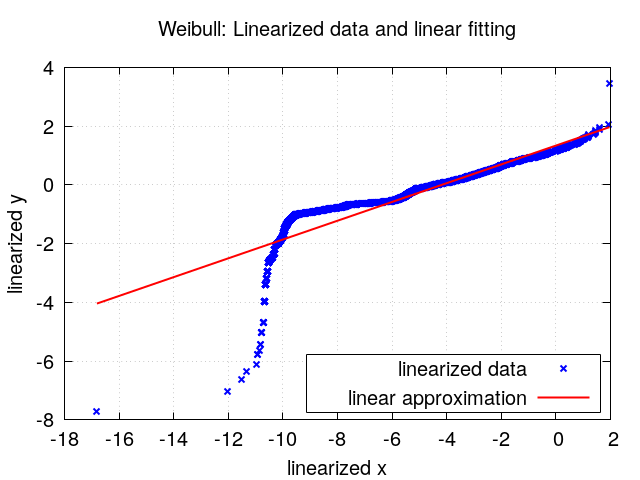
\includegraphics[height=50mm]{figures/ch4/Skype_Weibull_-_Linearized_data_and_linear_fitting}
  \label{fig:linearization}
}
%\hspace{0mm}
\subfloat[Cost function of the linear regression]{
  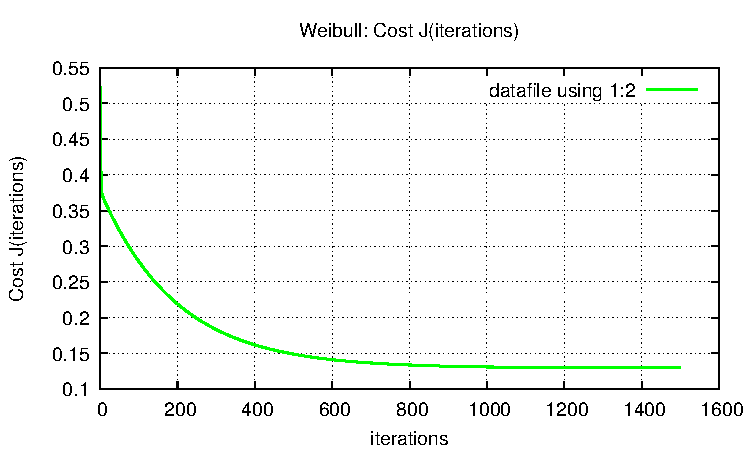
\includegraphics[height=50mm]{figures/ch4/Skype_Weibull_-_Cost_J_iterations__convergence}
  \label{fig:cost}
}
\label{fig:linearization-cost}
\caption{Linearized data and cost function of weibull linear regression}
\end{figure}



\subsubsection{Direct Estimation}

%2nd-review
The expected value $E(X)$ and variance $Var(X)$ of a random variable $X$ of some distributions are close related with its parameters. Since the mean $\bar{\mu}$ and its standard deviation $\bar{\sigma}$ are in general good approximations for the expected value and variance, we use them to estimate parameters.

%2nd-review
Following the notation presented at table~\ref{tab:distributions-equations}, we have for the normal distribution:
\begin{equation}
(\hat{\mu}, \hat{\sigma} = (\bar{\mu}, \bar{\sigma})
\end{equation}

%2nd-review
For the exponential distribution $E(X) = \frac{1}{\lambda}$, therefore we have:
\begin{equation}
\hat{\lambda} = \frac{1}{\hat{\mu}}
\end{equation} 

\subsubsection{Maximum Likelihood}

%2nd-review
The maximum likelihood estimation, is a method for estimation of parameters, winch maximizes the likelihood function. We explain in details this subject in the Appendix A. Using this method for the Pareto distribution, it is possible to derive the following equations the its parameters:

\begin{equation}
\hat{x_{m}} = \min_{i = 0, ..., m}\{x_{i}\}
\end{equation} 

\begin{equation}
\hat{\alpha} = \frac{n}{ \sum_{i = 0}^{m}(\ln{(x_{i}) - \ln(\hat{x_{m}})})  }
\end{equation} 

where $m$ is the sample size.


%\subsubsection{AIC and BIC}


\subsection{Modelling Method Validation}

%2nd-review
To see if our criterion of parameter selection is actually is able to find which is the best model, we define a validation methodology. 
We generate a vector with the same size form the original, with random generated data through our model estimation. Then we compare it with the original sample, trough four different metrics, all with a confidence interval of 95\%:

%2nd-review
\begin{itemize}
\item Correlation between the sample data and the estimated model (Pearson's product-moment coefficient);
\item Hurst exponent;
\item Mean inter packet time;
\item Standard deviation of inter packet times.
\end{itemize}

%2nd-review
The Pearson's product-moment coefficient, or simply correlation coefficient,  is an expression of the dependence or association between two datasets. Its value goes from -1 to +1. +1 means a perfect direct linear correlation. -1 indicates perfect inverse linear correlation. 0 means no linear correlation. So, as close the result reach 1, more similar are the inter-packet times to the original values. To estimate it, we use the Octave's function \texttt{corr()}.

%2nd-review
As explained before in the chapter~\ref{ch:literature-review}, the Hurst exponent is meter self-similarity and indicates the fractal level of the inter-packet times. As close the result is from the original, more similar is the fractal level of the estimated samples from the original.To estimate this value we use the function \texttt{hurst()} from Octave, which uses rescaled range method.
Finally we measure the mean and the standard deviation (as a measure of the dispersion), using the Octave's functions \texttt{mean()} and \texttt{std()}. We also present some \textit{QQplots}, to visually compare the random-generated data and the original dataset. 

%2nd-review
As close the correlation, Hurst exponent, mean and the standard deviation is from the original dataset, the better is model fitting. Also, analyzing the mean, we can see if a certain modeling procedure tends to be more penalized for the values close, or far from zero. This means that if the mean inter-packet time tends to be smaller or higher compared to the original. 

%2nd-review
With these results in hands, we can see if AIC and BIC are good criteria for model selection for inter-packet times. To quantitatively check it, we define a cost function based on the correlation, Hurst exponent and mean. We exclude the standard deviation, because the Hurst exponent being a meter of the fractal level, also capture information about the desired dispersion of the data. So, for comparing all these results, we defined a cost function $J$, based on the randomly generated data values.

%2nd-review
Being $Cr$ the vector of correlations ordered from the greater to the smaller. Let $Me$ and $Hr$ defined by the absolute difference between mean and hurt exponent of the estimated values and the original dataset. Both are ordered from the smaller to the greatest values. Letting $\phi(V, M)$ be an operator wich gives the position of a model $M$ in a vector $V$, we define the cost function $J$ as:


\begin{equation}
J(M) = \phi(Cr, M) + \phi(Me, M) + \phi(Hr, M)
\end{equation}

%2nd-review
The smaller is the cost $J$, the best is the model. Then we compare the results achieved by AIC and BIC, and $J$.

\subsection{Modelling Results}


%%%%%%%%%%%%%%%%%%%%%%%
% Logscale Skype
\begin{figure}[ht!]
\centering
\label{fig:aproximation-original-cdf}
\subfloat[Chauchy]{
  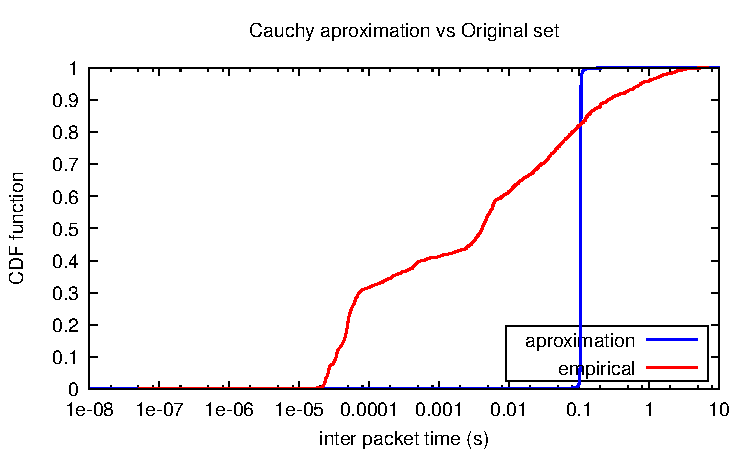
\includegraphics[width=78mm]{figures/ch4/Skype_Logscale_-_Cauchy_aproximation_vs_Original_set}
}
\subfloat[Exponential(LR)]{
  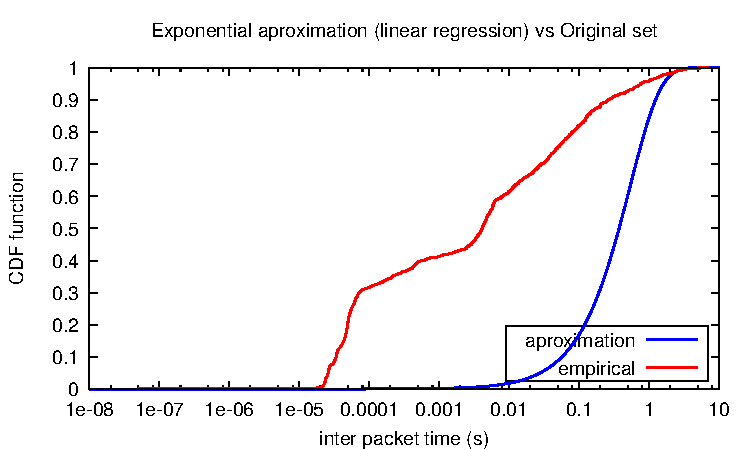
\includegraphics[width=78mm]{figures/ch4/Skype_Logscale_-_Exponential_aproximation__linear_regression__vs_Original_set}
}
\hspace{0mm}
\subfloat[Exponential(Me)]{
  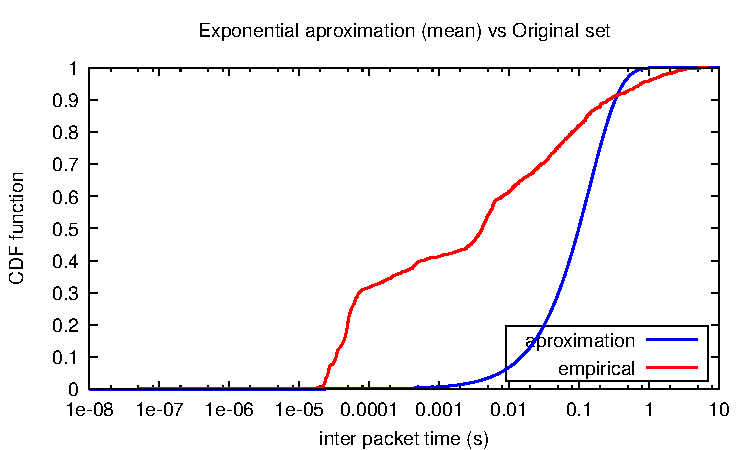
\includegraphics[width=78mm]{figures/ch4/Skype_Logscale_-_Exponential_aproximation__mean__vs_Original_set}
}
\subfloat[Normal]{
  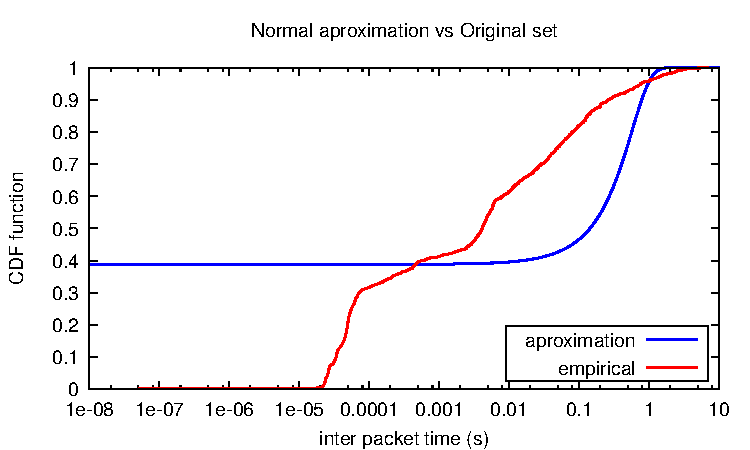
\includegraphics[width=78mm]{figures/ch4/Skype_Logscale_-_Normal_aproximation_vs_Original_set}
}
\hspace{0mm}
\subfloat[Pareto(LR)]{
  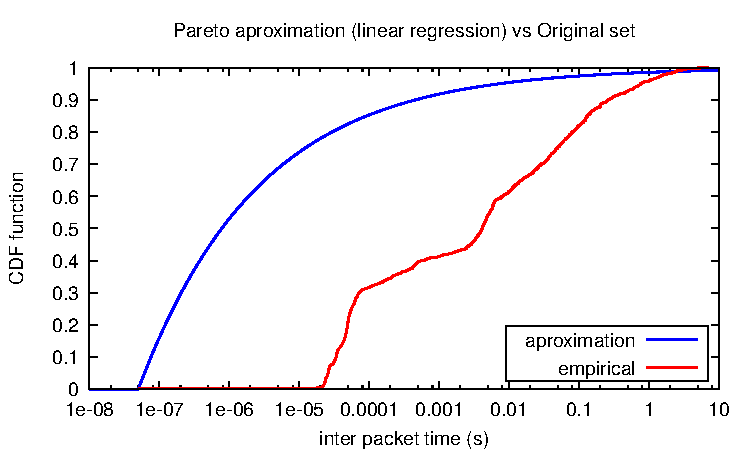
\includegraphics[width=78mm]{figures/ch4/Skype_Logscale_-_Pareto_aproximation__linear_regression__vs_Original_set}
}
\subfloat[Pareto(MLH)]{
  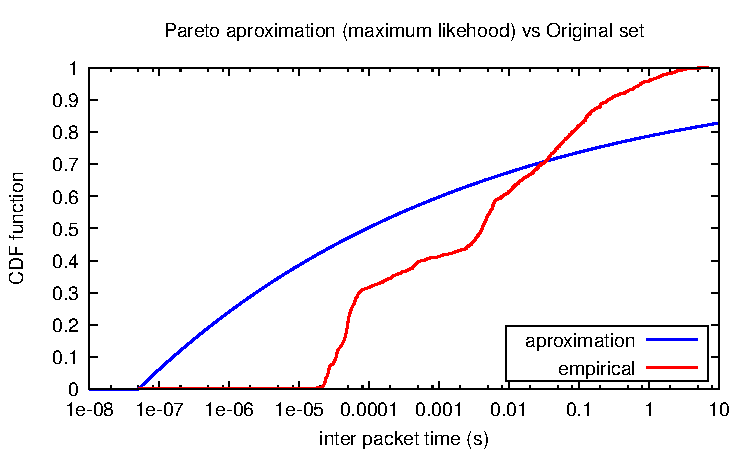
\includegraphics[width=78mm]{figures/ch4/Skype_Logscale_-_Pareto_aproximation__maximum_likehood__vs_Original_set}
}
\hspace{0mm}
\subfloat[Weibull]{
  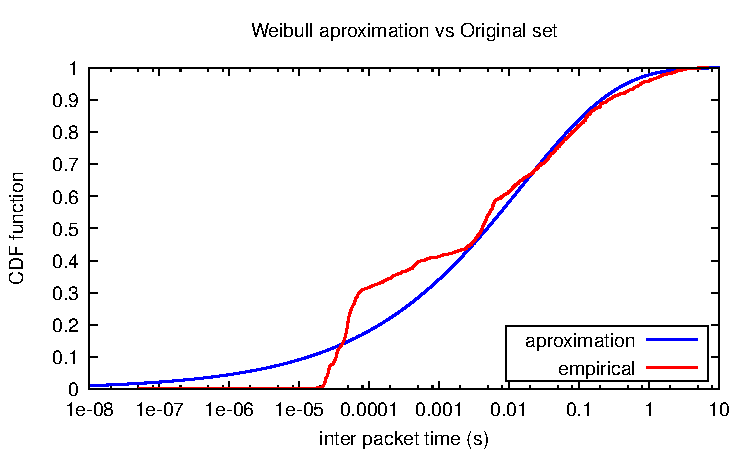
\includegraphics[width=78mm]{figures/ch4/Skype_Logscale_-_Weibull_aproximation_vs_Original_set}
}
\caption{CDF functions for the approximations of \textit{skype-pcap} inter  packet times, of many stochastic functions.}
\end{figure}


\begin{figure}[ht!]
	\centering
	\label{fig:qq-skype}
	\subfloat[Chauchy]{
		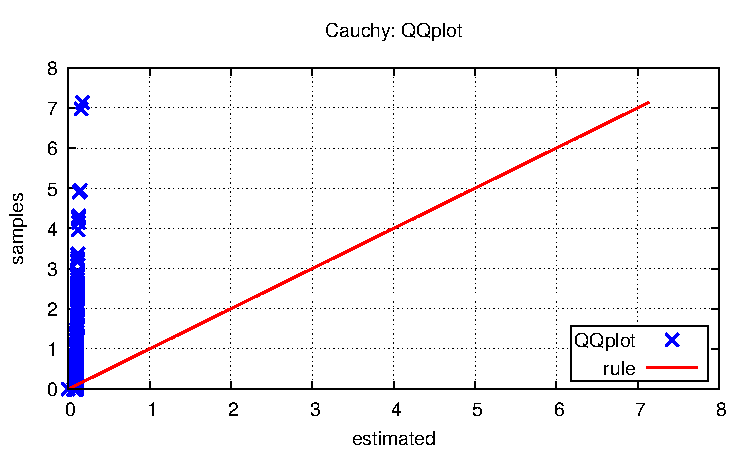
\includegraphics[width=78mm]{figures/ch4/skype_QQplot_-_Cauchy}
	}
	\subfloat[Exponential(LR)]{
		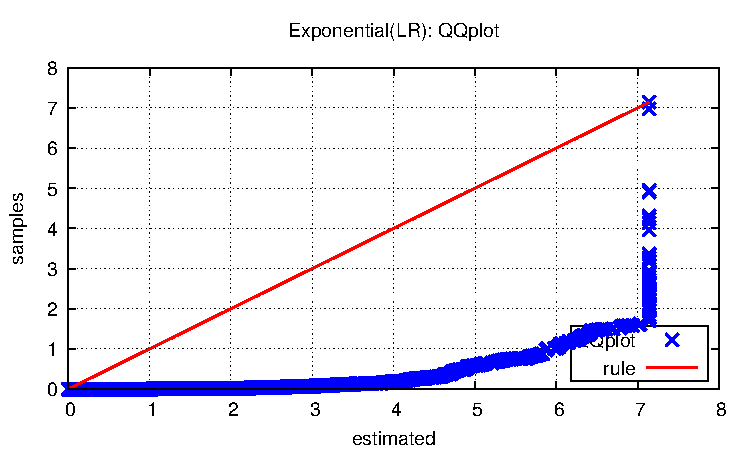
\includegraphics[width=78mm]{figures/ch4/skype_QQplot_-_Exponential_LR}
	}
	\hspace{0mm}
	\subfloat[Exponential(Me)]{
		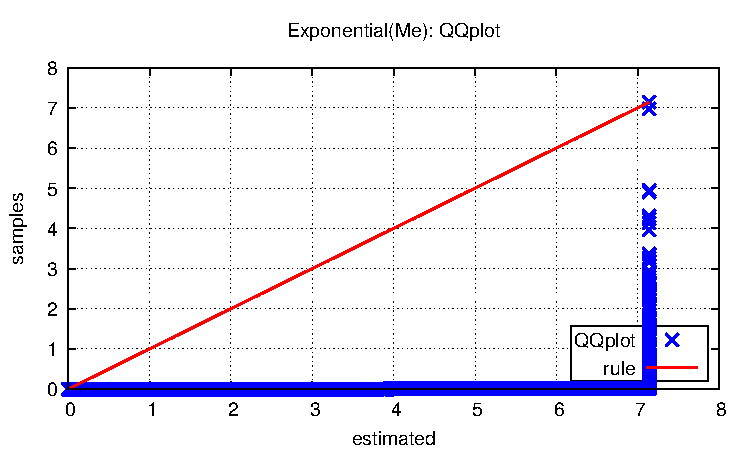
\includegraphics[width=78mm]{figures/ch4/skype_QQplot_-_Exponential_Me}
	}
	\subfloat[Normal]{
		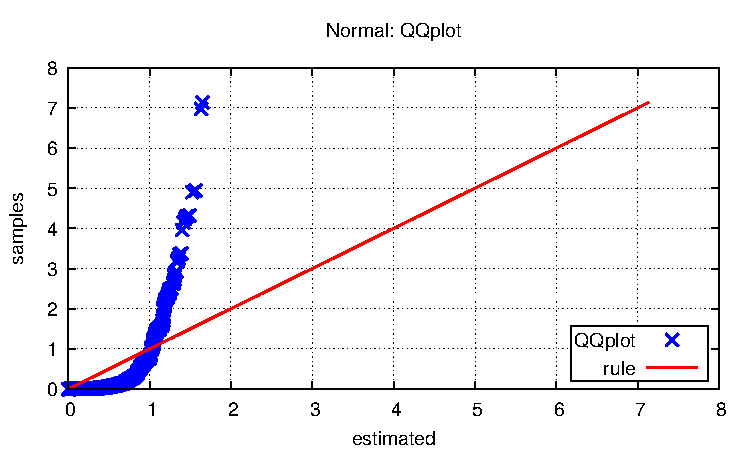
\includegraphics[width=78mm]{figures/ch4/skype_QQplot_-_Normal}
	}
	\hspace{0mm}
	\subfloat[Pareto(LR)]{
		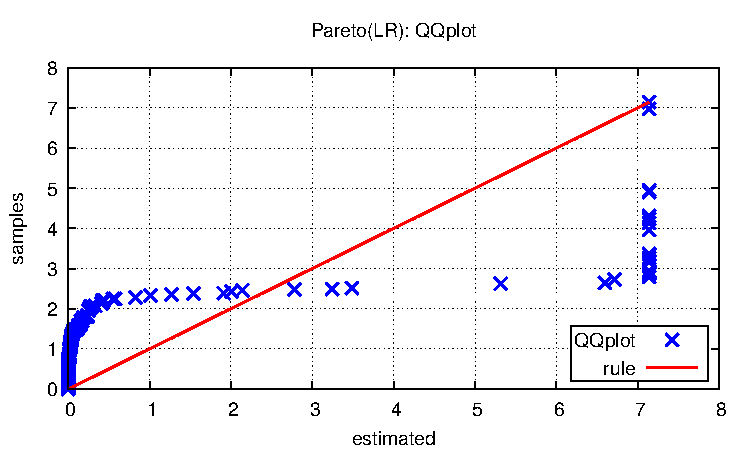
\includegraphics[width=78mm]{figures/ch4/skype_QQplot_-_Pareto_LR}
	}
	\subfloat[Pareto(MLH)]{
		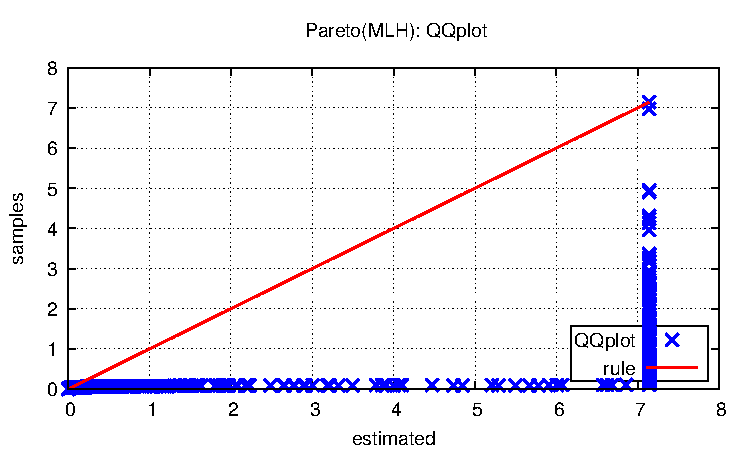
\includegraphics[width=78mm]{figures/ch4/skype_QQplot_-_Pareto_MLH}
	}
	\hspace{0mm}
	\subfloat[Weibull]{
		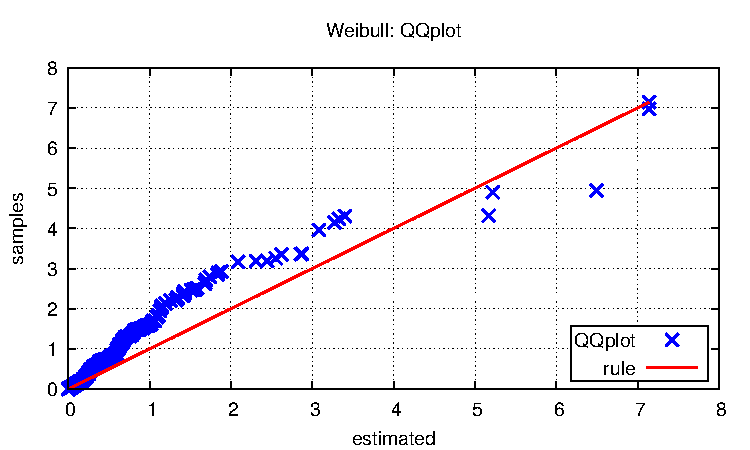
\includegraphics[width=78mm]{figures/ch4/skype_QQplot_-_Weibull}
	}
	\caption{CDF functions for the approximations of \textit{skype-pcap} inter  packet times, of many stochastic functions.}
\end{figure}


%%%%%%%%%%%%%%%%%%%%%%%
% Prototype results
\begin{table}[h!]
	\centering
	\caption{Results of the octave prototype, include BIC and AIC values, para estimated parameters for two of our pcap traces: \textit{skype-pcap }and \textit{bigflows-pcap}. \textit{bigflows-pcap} is much larger, and has a much much smaller mean inter-packet time}
	
	\scalebox{0.75}{ 
		\begin{tabular}{lcccccccc}
			\hline
			& \multicolumn{8}{c}{Trace} \\ \cline{2-9} 
			Function		& AIC  & BIC  & \multicolumn{2}{c}{Parameters}  
			& AIC & BIC  & \multicolumn{2}{c}{Parameters} \\ \hline 
			
			& \multicolumn{4}{c}{skype-pcap}  & \multicolumn{4}{c}{lan-diurnal-pcap}   \\ \hline 
			Cauchy          & $2.18e4$    & $2.19e4$    & $\gamma:2.59e-4$ & $x_0:1.05e-1$    
			& $-2.85e7$   & $-2.85e7$   & $\gamma:9.63e-3$ & $x_0:-3.61e-3$    \\
			Exponential(LR) & $-1.61e3$   & $-1.60e3$   & \multicolumn{2}{c}{$\lambda:1.86$}   
			& $1.79e6$    & $1.79e6$    & \multicolumn{2}{c}{$\lambda:8.51e-1$}    \\
			Exponential(Me) & $-4.29e3$   & $-4.28e3$   & \multicolumn{2}{c}{$\lambda:7.01$}   
			& $-3.12e7$   & $-3.12e7$   & \multicolumn{2}{c}{$ \lambda:58.78$} \\
			Normal          & $3.29e3$    & $3.31e3$    & $\mu:1.43e-1 $    & $\sigma:5.01e-1$ 
			& $Inf$       & $Inf$       & $\mu:1.70e-2$     & $\sigma:8.56e-2$ \\
			Pareto(LR)      & $-8.28e3$   & $-8.27e3$   & $\alpha:2.52e-1$ & $x_m:5e-8$    
			& $-4.60e7$   & $-4.60e7$   & $\alpha:2.55e-1$ & $ x_m:5e-8$    \\
			Pareto(MLH)     & $-1.16e4$   & $-1.16e4$   & $\alpha:9.21e-2$ & $x_m:5e-8$    
			& $-5.03e7$   & $-5.03e7$   & $\alpha:1.15e-1$ & $ x_m:5e-8$    \\
			Weibull         & $-1.46e4$   & $ -1.46e4$  & $\alpha:3.20e-1$ & $\beta:1.52e-2$  
			& $-5.60e7$   & $-5.60e7$   & $\alpha:3.34e-1$ & $\beta:1.83e-3$  \\ \hline	
			& \multicolumn{4}{c}{bigFlows-pcap} & \multicolumn{4}{c}{wan-pcap}  \\ \hline
			Cauchy          & $7.14e6$    & $7.14e6$   & $\gamma:1.94e0$ &$x_0:-7.25$    
			& $5.99e7$    & $5.99e7$   & $ \gamma:8.28e2$ &$x_0:-4.52e3$    \\
			Exponential(LR) & $7.33e6$    & $7.33e6$   & \multicolumn{2}{c}{$\lambda:1.489e-1$}   
			& $5.68e7$    & $ 5.68e7$  & \multicolumn{2}{c}{$\lambda:2.2e-5$}   \\
			Exponential(Me) & $-1.09e7$   & $-1.09e7$  & \multicolumn{2}{c}{$\lambda:2.64e3$}   
			& $-6.58e7$   & $-6.58e7$  & \multicolumn{2}{c}{$\lambda:6.58e5$} \\
			Normal          & $-9.35e6$   & $-9.35e6$  & $\mu:3.79e-4$   &$\sigma:6.60e-4$ 
			& $-6.39e7$   & $-6.39e7$  & $\mu:2e-6$     & $\sigma:1e-6$ \\
			Pareto(LR)      & $-1.02e7$   & $-1.02e7$  & $\alpha:1.489e-1 $ & $x_m:5e-8 $    
			& $-5.31e7$   & $-5.31e7$  & $\alpha:NaN$ & $x_m:5e-8 $    \\
			Pareto(MLH)     & $-1.03e7$   & $-1.03e7$  & $\alpha:1.362e-1$ & $x_m:5e-8 $    
			& $-6.25e7$   & $-6.25e7$  & $\alpha:3.39e-1$ & $x_m:5e-8 $    \\
			Weibull         & $-1.10e7$   & $-1.10e7$  & $\alpha:2.81e-1$ & $\beta:5.54e-4$  
			& $-5.46e7$   & $-5.46e7$  & $\alpha:7.64e-2$ & $\beta:1e-6$  \\ \hline
		\end{tabular}
	\label{tab:prototype-results}
	}
\end{table}

Here in this chapter we only discuss the plots achived obtained by the pcap \textit{skype-pcap} for simplicity. The other plots are provided and commented on the appendix ~\ref{ap:aditional-plots}. In the figure ~\ref{fig:aproximation-original-cdf} we present all estimated CDF functions along with the empirical CDF, for the trace \textit{skype-pcap}. They are on logscale, wich provide a better visualization for small time scales. In the case of the normal function, all values smaller than zero, were set to zero on the plot. Is possible to see different accuracies and types of fittings on each plot. Visually, the best fit seems to be the Weibull trough linear regression. 

Analyzing the plots, and what they would mean, our Cauchy fitting would impose an almost contant traffic , with the inter packet time close to the mean. On the trace \textit{skype-pcap} the exponential plots seems to not represent well the small values of inter packet times. This is due fact that an exponential process is good at representing values close to the mean. But, it fails to represent values too small and higher. On the other hand, a self-similar process like Weibull and Pareto are better representing inter packet times with higher dispersion. Pareto(MLH) has a slow convergence, wich means this distribution may genarate values of inter-packet times too large. 

Analyzing the QQplots, we may observe that in most of the distribution, the samples (original data) has a much havier-tail effect than in the estimated data. This is verified by the almost blue horizontal lines formed by the "exes". But, the Weibull distribution follow much closer the original data. Also is possible to see that the sample has a right skew compared to the estimation on Exponential(LR), Exponential(Me), Normal, and Pareto(MLH). This means that this estimation would not represent so well small values of time in this case. On the other hand, Pareto(LR) and Weibull would not suffer from this problem.

The results for the AIC, BIC and parameters of all four traces are at the table~\ref{tab:prototype-results}.  The results for \textit{wan-pcap} and \textit{lan-diurnal-pcap} are on the table ~\ref{tab:prototype-results}. The difference between BIC and AIC values in all simulations are very small. Much smaller then the difference of these values between the distributions. This is an indication that for inter packet times, using AIC or BIC should will not influence significantly the results. 

On our previsions, Weibull and Pareto(MLH and LR) are the best options. This was expected, since both are heavy-tailed functions. But Cauchy on most of the tests, even being a heavy-tailed distribution, seems to no present a good fitting. This is effect of the fast divergence of tangent function, when we linearize our data. 

Analyzing the quality of AIC and BIC as criterion of choose on \textit{skype-pcap},based on the results form figure ~\ref{fig:correlation-hurst-skype-pcap} we see that in therms of Correlation and Self-similarity it picket the right model: Weibull. Also in therms of mean packet rate and dispersion it is still one of the best choises (along with Exponential(Me), Pareto(LR) and Cauchy). The third and the fourth choices (Pareto(LR)) and Exponential(LR) also are good options in most of these metrics. But, Pareto(MLH) is presented as the second best choice, and it had poor results in comparison to the others, especially on mean, correlation and dispersion. 

All these results are abstracted by the cost function $J$. As we can see, on all pcaps, the best function selected by BIC and AIC~\ref{tab:prototype-results} also had the small cost~\ref{fig:cost-function}. 

Another important observation is the fact that exponential function was able to provide the best fitting for the \textit{wan-pcap}. The reasons for this behavior are both result of a much intense traffic with no long-range gaps, and the precision of the measurement.

%%%%%%%%%%%%%%
% Skype correlation, Hurst, Mean Standard Deviation
\begin{figure}[t!]
	\centering
	\subfloat[Correlation]{
		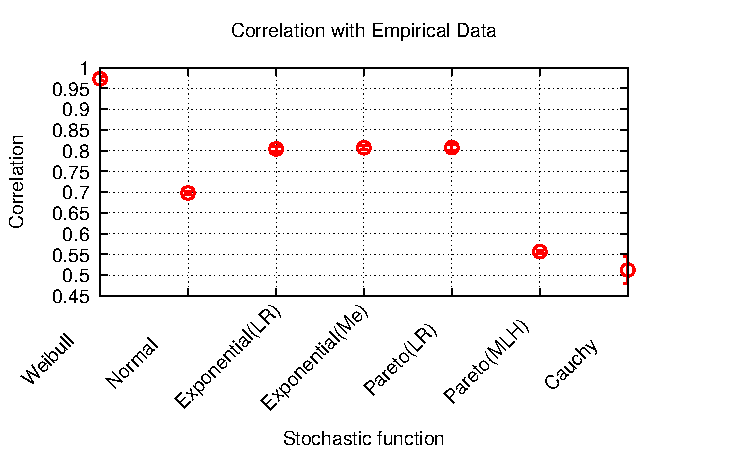
\includegraphics[width=75mm]{figures/ch4/Skype_Correlation}
		\label{correlation-skype}
	}
	\hspace{0mm}
	\subfloat[Hust Exponent]{
		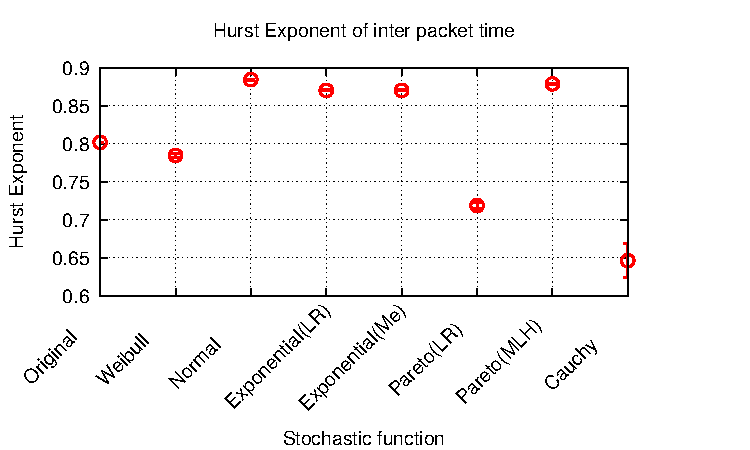
\includegraphics[width=75mm]{figures/ch4/Skype_Hurst_Exponent}
		\label{hurst-skype}
	}
	\hspace{0mm}
	\subfloat[Mean]{
		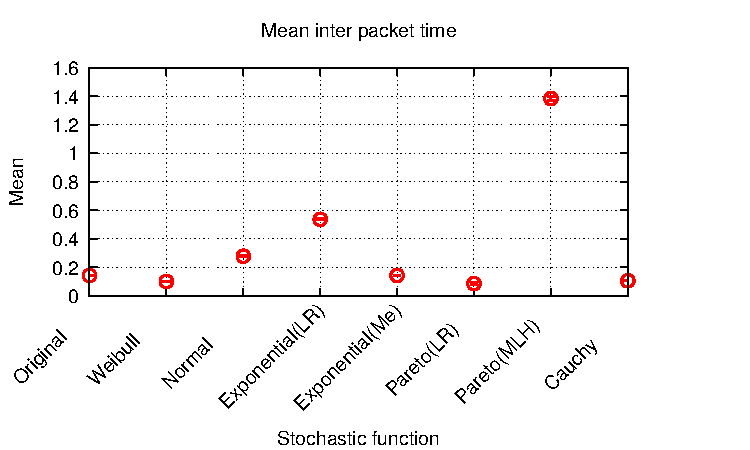
\includegraphics[width=75mm]{figures/ch4/Skype_Mean}
		\label{mean-skype}
	}
	\hspace{0mm}
	\subfloat[Standard Deviation]{
		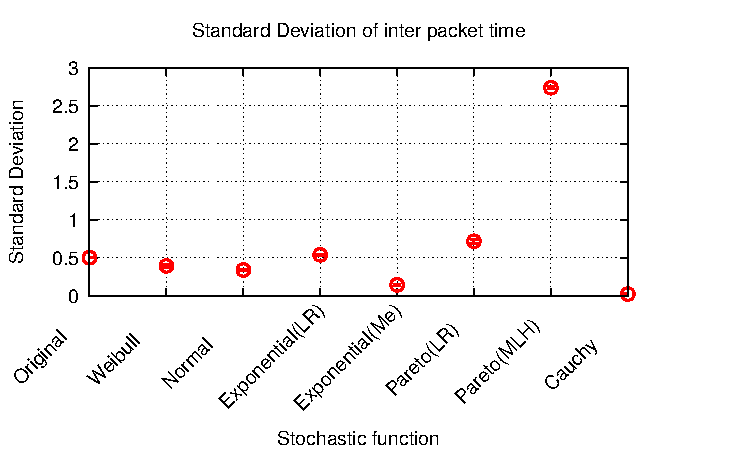
\includegraphics[width=75mm]{figures/ch4/Skype_Standard_Deviation}
		\label{std-skype}
	}
	\caption{Statistical parameters of \textit{skype-pcap} and its approximations}
	\label{fig:correlation-hurst-skype-pcap}
\end{figure}

%validation Cost function
\begin{figure}[t!]
	\centering
	\subfloat[\textit{skype-pcap}]{
		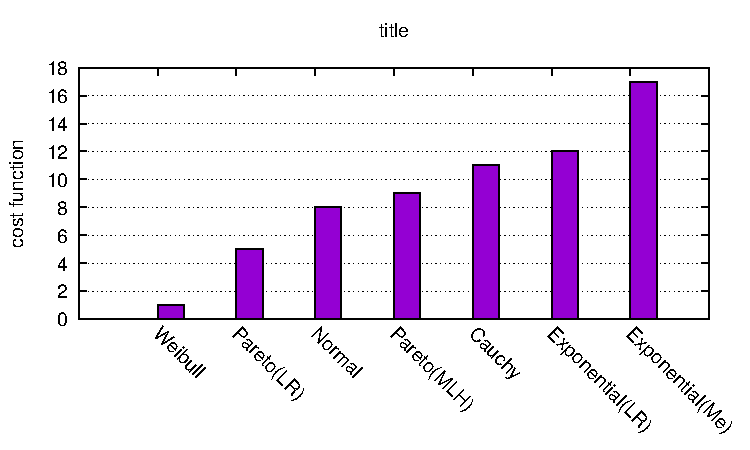
\includegraphics[width=75mm]{figures/ch4/Skype_costFunction}
		\label{cost-skype-pcap}
	}
	\hspace{0mm}
	\subfloat[\textit{bigFlows-pcap}]{
		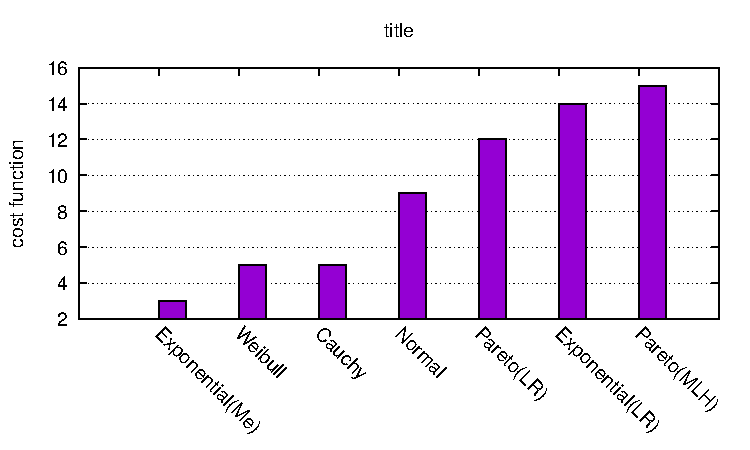
\includegraphics[width=75mm]{figures/ch4/bigFlows_costFunction}
		\label{cost-bigFlows-pcap}
	}
	\hspace{0mm}
	\subfloat[\textit{lan-diurnal-pcap}]{
		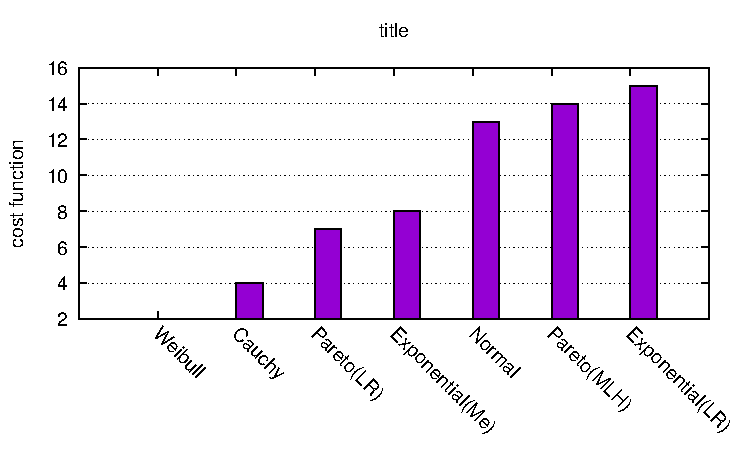
\includegraphics[width=75mm]{figures/ch4/Lan_costFunction}
		\label{cost-lan-pcap}
	}
	\hspace{0mm}
	\subfloat[\textit{wan-pcap}]{
		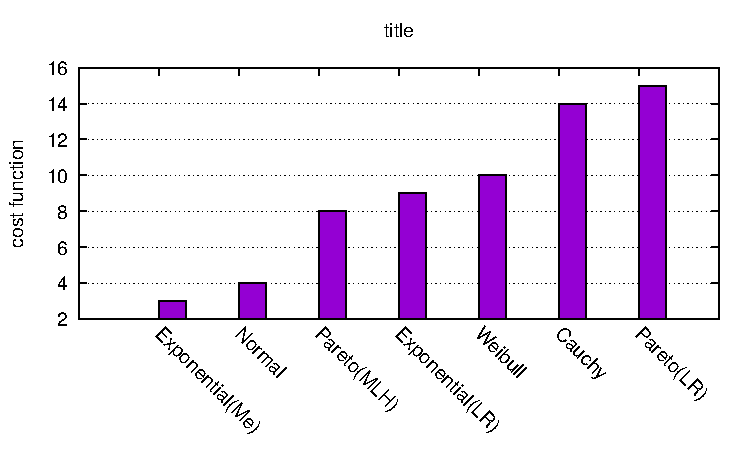
\includegraphics[width=75mm]{figures/ch4/Wan_costFunction}
		\label{cost-wan-pcap}
	}
	\caption{Cost function for each one of the datasets used in this validation process}
	\label{fig:cost-function}
\end{figure}

\begin{algorithm}[ht!]
	\caption{stochasticModelFitting}
	\label{alg:stochasticModelFitting}
	\begin{algorithmic}[1]
		\small		\Function{stochasticModelFitting}{$interArrivalData, criterion$}
		\State $m = interArrivalData.size$
		\State $interArrivalData = interArrivalData + MIN\_TIME$
		\If{$m < MINIMUM\_AMOUNT\_OF\_PACKETS$}
		\State $model\_list = \{constant\}$
		\Else
		\State $model\_list = \{weibull, pareto\_lr, pareto\_mlh, exponential\_me, exponential\_lr, normal,$
		\State $cauchy, constant\}$
		\EndIf
		
		\For{$model$ \textbf{in} $model\_list$}
		\State $model.fitting\_model(interArrivalData)$
		\EndFor
		\State $model\_list.sort(criterion)$
		\State \textbf{return} $model\_list$
		\EndFunction
	\end{algorithmic}
\end{algorithm}


\subsection{Conclusion}



We are able to conclude that using AIC or BIC as criteria for choosing models for inter-packet times is a good choise.

Except by the Pareto function modeled using the Maximum likelihood method, have comparative results between the simulations and the AIC/BIC goes. The best fittings according to the AIC/BIC usually returned very accurate models, with a small error between the mean and fractal level, and correlation close to one. The models selected as the worsts usually returned poor results.

It is important to notice that in some cases, some stochastic functions may perform poorly, and in other provide an accurate fitting, what justify the application of the criteria in all new experiments. For example, Weibull usually performs pretty well, but in some cases, perform poorly, and in others may even diverge. 

We do not rely on only one type of parameterization. This turns our methodology more robust, since a linear regression may diverge. But always there will be a peaceable model, since our estimations for Normal, Exponential (Me) and Pareto (MLH) cannot. Models which the linear regression diverges, will have very high and positive BIC/AIC estimations, and will not stand as primary options.


\section{ON/OFF Periods and Application classification}

	
\begin{algorithm}[ht!]
	\caption{calcOnOff}
	\label{alg:calcOnOff}
	\begin{algorithmic}[1]
		\small
		\Function{calcOnOff}{$arrivalTime, deltaTime, cutTime, minOnTime$}%\Comment{Where A - array, p - left, q - middle, r - right}
		\State $m = deltaTime.length() - 1$
		\State $j = 0$
		\State $lastOff = 0$
		\State $pktCounterSum = 0$
		\State $fileSizeSum = 0$
		\For{$i = 0:m$}
		\State $pktCounterSum = pktCounterSum + 1$
		\State $fileSizeSum = fileSizeSum + psSizeList[i, 1]$
		\If{$deltaTime[i] > cutTime$} 
		\If{$i == 1$} \Comment{if the first is session-off time}
		\State $j++$
		\State $onTimes.push(minOnTime)$
		\State $offTimes.push(deltaTime[i])$
		\State $pktCounter.push(pktCounterSum)$
		\State $fileSize.push(fileSizeSum)$
		\State $pktCounterSum = 0$
		\State $fileSizeSum = 0$
		\Else \Comment{base case} 
		\State $pktCounter.push(pktCounterSum)$
		\State $fileSize.push(fileSizeSum)$
		\State $pktCounterSum = 0$
		\State $fileSizeSum = 0$
		\If{$j == 0$}
		\State $onTimes.push(arrivalTime[i - 1])$
		\State $offTimes.push(deltaTime[i])$
		\Else \Comment{others on times} 
		\State  $onTimes.push(max(deltaTime[i-1] - deltaTime[lastOff], minOnTime))$ 
		\State  $offTimes.push(deltaTime[i])$
		\EndIf
		\State $lastOff = i$
		\EndIf 
		\EndIf       
		\EndFor
		\State $pktCounterSum = pktCounterSum + 1$
		\State $fileSizeSum = fileSizeSum + psSizeList[m]$
		\If{$lastOff == m - 1$} \Comment{ if last is session-off }
		\State $onTimes.push(minOnTime)$ % on time
		\Else \Comment{ base last case}
		\If{$lastOff \neq 0$}
		\State $onTimes.push(arrivalTime[m] - arrivalTime[lastOff])$ 
		\Else 
		\State $onTimes.push(arrivalTime[m])$ \Comment{there was just on time}
		\EndIf
		\EndIf
		\State $pktCounter.push(pktCounterSum)$
		\State $fileSize.push(fileSizeSum)$
		\State \textbf{return} $onTimes, offTimes, pktCounter, fileSize$
		\EndFunction
	\end{algorithmic}
\end{algorithm}
	
\begin{table}[ht!]
	\centering
	\caption{Application matach table}
	\label{tab:application-protocols}
	\begin{tabular}{lll}
		\hline
		Application Protocol & Transport Protocols & Transport Ports \\ \hline
		HTTPS               & TCP                & 443             \\
		FTP                 & TCP                & 20, 21          \\
		HTTP                & TCP                & 80              \\
		BGP                 & TCP                & 179             \\
		DHCP                & UDP                & 67, 68          \\
		SNMP                & UDP, TCP           & 161             \\
		DNS                 & UDP, TCP           & 53              \\
		SSH                 & UDP, TCP           & 22              \\
		Telnet              & UDP, TCP           & 23              \\
		TACACS              & UDP, TCP           & 49              \\ \hline
	\end{tabular}
\end{table}




In this section we breef show another methods used by the \textit{TraceAnalyzer} component. The first to calculate the session ON and OFF times. The second classify applications based on its tranport protocol and ports. In the table ~\ref{tab:methods} we summarize the stack of models used to create the Compact Trace Descriptor (CTD file). 



We developed an algorithms to calculate the times between the ON and OFF times of the \textit{files}, and the number of packets and bytes as well. It uses a list of packet arrival times(relative to the first), time between packets and packet sizes. It defines a minimum time of ON acceptable. This times is used for two reasons:

\begin{itemize}
\item In case of a \textit{file} of just one packet, it will not produce a On time of zero
\item It avoid a \textit{file} On time too small, wich may be less than acceptable for packet generator tools.
\end{itemize}

As explained in the previous chapter, a \textit{file} is defined by a large OFF time, we call $cutTime$. If a inter packet $deltaTime$ time is larger than the $cutTime$ it defines an OFF time, and the ON time is calculated base on the last OFF time recorded. 
If the first $deltaTime$ defines an OFF time, or if it is the first ON time, its calculation is threated separetely. In the last ON time, it is not defined by an OFF time, so we deal with it after the loop. It keep counters to calc the number of bytes and packets within every defined ON time. It returns four vectors: $onTimes$, $offTimes$, $pktCounter$ and $fileSize$. Letting $n$ be the size of $onTimes$,  $offTimes$ has a size $n - 1$. The algorithm is presented in the Alforithm~\ref{alg:calcOnOff}.



We also developed an simple test to guess the application protocol, based on the port numbers and the tranport protocol used by each flow. We currently are classifing the application protocols presented in the table ~\ref{tab:application-protocols}. If a flow matches the port number, and the transport protocol, it is classified as belongig to an application protocol.

\section{Conclusions}

In this section, we went on details on some methodologies mentioned in the chapter ~\ref{ch:architecture}. Here we avoid implementation and architecture concepts, and just discussed the methods. In this first section, we focused our research on develope a consistent method for automatic selection of stochastic functions for inter-packet times. Since we could not find any other methodology in the literature, we developt our own and tested if it is worth or not. The results showed our method satisfactory and had presented a reasonable prediction rate on the best functions. We now can ensure that it is a safe method and that AIC and BIC are good criterions for this sort of data.  We abstracted this method in the algorithm ~\ref{alg:stochasticModelFitting}. In the second section, we also present the methods used to estimate packet trains periods (algorithm ~\ref{alg:calcOnOff}) and make the application classification (table ~\ref{tab:application-protocols}). In the table ~\ref{tab:methods}, the usage of each method is summarized. 

\begin{table}[ht!]
	\centering
	\caption{Methods used by each layer.}
	\label{tab:methods}
	\begin{tabular}{cc}
		\hline
		Layer                               & Method                                 \\ \hline
		Link Layer                          & \multirow{3}{*}{Packets header's data} \\
		Network Layer                       &                                        \\
		Transport Layer                     &                                        \\
		Application Layer                   & Application Match Table                \\
		\multirow{2}{*}{Inter Packet Times} & Algorithm: $calcOnOff$                 \\
		& Algorithm: $stochasticModelFitting$    \\
		Packet Sizes                        & Algorithm: $stochasticModelFitting$    \\ \hline
	\end{tabular}
\end{table}

%\section{Implementation Details}

%\subsection{Modeling Process}

%\subsection{Matlab prototyping and C++ Implementation}

%\subsection{Software Engineering process and Lessons Leaned}

%\section{Conclusion}

%We can conclude by this evaluation, that our chosen methodology for selecting stochastic models for inter packet data is appropriated. The first thing to observe is that, for a high 

%First, we do not rely on only one type of parametrization. This turns our methodology more robust, since a linear regression may diverge. But aways there will be an packable model, since our estimations for Normal, Exponential(Me) and Pareto(MLH) cannot. Models wich the linear regression diverge, will not have god BIC/AIC estimations, and will not be picked. 

% https://en.wikipedia.org/wiki/Gamma_process
%Intordução
%- Como previamente discutido, há uma farta bibliografia dedicada ao estudo da natureza do trafego de internet. Em especial, relacionada a modelos que possam expressar a natureza do tempos entre pacotes. 
%- Como discutido anteriormente, Sabemos pela literatura que o trafego de internet possui uma caracteristica fractal. Processos tipicos de Poisson (expresso em sua forma contínua por uma funções estocastica esponencial)  não são capazes de representar de maneira realistica o trafego. Para tal, podem ser utilizados processos estocasticos heavy-tailed.
%- Porém não são numerosos os trabalhos que tratam da parametrização desses processos. Qual o melhor tipo de parametirzação é uma questão difícil de ser respondida, por diversas. Primeiramente, utilizar funções heavy-tailed pode ser uma metodologia mais eficaz para se garantir a self-similarity do trafego. Porém não necessáriamente outras importantes características do trafego serão mantidas, como por exemplo: média de pacotes por segundo, disperssão e correlação entre o trafego real e o trafego sintético gerado por esse processo. Não há a prncípio uma carantia que a escolha baseada em self-similatrity também irá garantir que essas outras características se mantanham. O ideal é que  encontremos um método que possa garantir um bom resultado na maioria, se não em todas essas características.
%- Além disso, há diversos métodos disponíveis para se estimar parâmertos de uma função estocastica. Para citar alguns exemplos:
%* Em alguamas funções como a normal e a exponencial os parâmetros podem ser estimados diratemente através do calculo da média e da variância dos dados.
%* Em funções que é possivel realizar a linearização, os parametros podem ser estimados por meio de regressão linear
%* Outro método frequentemente usado é o do maximum likelihood
%Porém, prever comportamento que cada funções estocástica terá com cada um desses estimadores, não é trivial. Por exemplo.  Por exemplo:
%* Dependendo dos dados originais, a estimativa pode ser muito pobre, e posuir uma baixa correlação com os dados originais. 
%* Os estimadores possuirão algum "bias", desviando apresentando um desvio para cima ou para baixo no valor esperado. Ou isso pode não ocorrer.
%- O objetivo desse capítulo é somente avaliar a qualidade de nosso modelo para estimativa de parâmetros estocasticos para estimadores de inter packet times. iremos utilizar o nosso procedimento em diferentes datasets, e avaliar a qualidade dos resultados obtidos.

\begin{comment}

%%%%%%%%%%%%%%

%To evaluate the quality of the generated data, we use four criteria: 

%As we can see in the figure~\ref{correlation-skype-pcap}, Weibull has a correlation close to one correlation (0.969). The follow values of next values of correlation are: Pareto(LR)(0.810), Normal (0.701), Exponential(LR) (0.697), Pareto(MLH) (0.556), Cauchy (0.470), and Exponential(Me) (0.294).

%The next criterion is The Hurst exponent. First, we can observe that all fittings have resulted in a  self-similar process since all values were between 0.5 and 1. Again, the AIC prediction was confirmed, since the Weibull fitting is the one with the closest fractal level from the original trace, around 0.80 and 0.85.

Revisão da literatura
* O trabalho do sourcesonoff realisa uma análise extensiva de uma modelagem apropriada entre bursts de trafego. No trabalho, algumas funções estocasticas são analizadas, e é recomendado o uso sa Weibull. Nesse trabalho é utilizado o calculo do prâmetro BIC como estimador da melhor função estocastica


Metodologia e validação
- por questões referentes a teoria da iinformação, optamos por utilizar o parametro AIC como nosso estimador oficial de melhor função estocastica. 
- Porém, também calculamos o BIC, e verificamos ue via de regra a diferença dos dois valores é bem baixa. Em geral, para datasets maiores, a diferença entre o BIC e AIC de uma mesma função tende a ser consideravelmente menor do que se comparado ao de outra funçao, como veremos a seguir
- A metodologia escolhida é a seguinte: realizamos a estimativa de parametors de diversas funções estocasticas para um mesmo dataset. Calcularemos o valor do AIC, e baseado nele, iremos estimar, em ordem crescente qual a melhor função estocástica. 
- fazer uma figura com cores, mostrando segundo o estimador a ordem das funções, e compara-las com  a ordem estimada por meio dos 4 outros parâmetros.
 - Utiizar correlação, media, variancia, e hurst.
- A vantagem do AIC é que tendo a disposição o datset original, ele é um metodo completamente analítico, não dependendo da geração de numeros aleatórios (como por exemplo no cauculo da correação). Nesse caso, evita que o gerador escolhido possua algum bias na geração dos dados, e comprometa o resultado do estimaor. Além disso, é um procedimento computacionalmente mais barato, pois é puramente analitico

Resultados
- Neste capítulo apresentaremos a análise de somente  2 datasets: da captura de skype e da captura big-flows. No apendice haverão outras análises, que incluem:
* uma análise de inter packets times de uma captura diurnal
* inter-packets times de um single flow do caida
* inter-burst timesconsiderando apenas inter-packet times maiores do que 1 segundo.
* inter pacekt time de 1 segundo do trace do caida.
- o porposito desse modelo é avaliar a qualidade do modelo de seleção, se ele é uma boa ou mpa escolha, já que não há muitso trabalhos relacionados na literatura.
- como o trafego de internet é fractal, caso essa metodologia represente uma boa escolha para os datsets analisados, ele também tende a ser uma boa escolha para datasets de diferentes intervalos de inter-packet times (maiores e menores). Uma análise mais precisa é feita no apendice a respeito dessa questão.






Conclusões







%In this chapter we will go deep into details on how our tool makes the data modeling, focusing on inter-packet times. We will present curves obtained by our Matlab prototype that shows in detail how each step works. After explaining this process, we will present an evaluation method of our results, using \textit{QQplots}. After this, we give some details of how we convert code from Matlab to C++ and its benefits on time execution. All code used in this section is available on our GitHub page, on the directory \texttt{Prototypes}. 

%We also define here the datasets we are going to use in the rest of this text. We will use two datasets, and for reproduction purposes, one is public available. The first is a CAIDA\footnote{http://www.caida.org/home/}{http://www.caida.org/home/}, and can be found at  \href{https://data.caida.org/datasets/passive-2016/equinix-chicago/20160121-130000.UTC}{https://data.caida.org/datasets/passive-2016/equinix-chicago/20160121-130000.UTC}. Access to this file need login, so you will have to create an account and wait for approval first. The pcap's file name is \texttt{equinix-chicago.dirA.20160121-130500.UTC.anon.pcap.gz}. The second we capture in our laboratory LAN, through a period of 24 hours. Along with other tests, We intend to verify diurnal behavior on it. 


%%%%%%%%%%%%%%%%%%%%%%%%%%%%%%%%%%%%%%%%%%%%%%%%%%%%%%%%%%%%%%%%%%%%%%%%%%%%%%%%


%After we implement this models, we where able to get different approximations for the stochastic functions. To evaluate how well the method is able to fit inter packet times, we first test it against a whole set of inter packet times. Figures (...) represents the CDF fitting for the function for the \textit{skype-pcap}. In the apendix ~\ref{ap:mathematical-modeling}, we also present the fitting achieved for whole set of inter-packet times, and for a single selected flow of \textit{caida-pcap} and\textit{lan-diurnal-pcap} \textit{pcaps} . We are able to see that the Weibull approximation fits better then any exponential approximation. But, we define an automatic way to estimate the best fitting. We  use the AIC (Akaike information criterion), winch is gave by:

%\begin{equation}
%AIC = 2k - 2\ln{(L)} 
%\end{equation} 

%where $k$ is the number os estimated parameters for the stochastic function, and $L$ is the value of the likelihood function. We explain it in details in the appendix A. The smaller is the AIC value, the best is the function fitting. An alternative for the AIC, is the BIC value, which follow the same rule. Big is defined by the equation:

%\begin{equation}
%BIC = k\ln{(n)} - 2\ln{(L)}
%\end{equation}

%where n is the number of elements of the sample dataset. We present at table ~\ref{tab:bic-aic} the values found by each estimator, for the \textit{skype-pcap}.

%As we can see, both BIC and AIC agree on each element, which one is the best and the worst. In this case, the best is the Weibull and the worst is the Cauchy. The exponential models, which are the continuous version of a classical Poisson process, is worse than Weibull and both Pareto estimation.

%But, to verify if our estimation is good, we need to see what sort of data these stochastic process are able to generate, and how close the stochastic properties of the synthetic dataset is from the original. In this way, we will be able to verify its actual quality in  unbiased way.



% The Pearson correlation is +1 in the case of a perfect direct (increasing) linear relationship (correlation), −1 in the case of a perfect decreasing (inverse) linear relationshi



%\textcolor{red}{TODO:Fazer uma breve avaliação das parametrizações obtidas com os dois traces utilizando QQplots, e comentar os resultados }


%\section{C codification}

%\textcolor{red}{TODO: Explicar detalhes da codificação em C, como bibliotecas utilizadas, a utilização de valores minimos para evitar o calculo de $\log{0}$, e a opção de executar testes de regressão, compilando com a opção regression-tests ou outra que eu criar na hora.}
\end{comment}

\bookmarksetup{startatroot}%
%%%%%%%%%%%%%%%%%%%%%%%%%%%%%%%%%%%%%%%%%%%%%%%%%%%%%%%%%%%%%%%%%%%%%%%%%%%%%%%%
\chapter{Proof of Concepts and Validation}\label{ch:validation}
%%%%%%%%%%%%%%%%%%%%%%%%%%%%%%%%%%%%%%%%%%%%%%%%%%%%%%%%%%%%%%%%%%%%%%%%%%%%%%%%

\section{Emulated Testbeds}


As first proof of concepts for our tool, we are going to use Mininet's emulated testbeds. These tests are easily implemented and reproduced, and are able to test the performance of our tool, without kernel and hardware overheads. Tests in a physical testbeds, and real network functions stays for future work.

This first testbed is a tree topology, and represents tests performed by Swing\cite{swing-paper} found on the literature \cite{background-traffic-matter}\cite{legotg-paper}. The second is much simples, and is just a one hop connection of two hosts. Both topologies are SDN neworks, and have OpenDayLight Beryllium as controller. 


All the traffic is generated by the host \textit{h1} with IPv4 address 10.0.0.1. The traffic will to be captured form the host interface with TCPdump in a pcap format, and just the outgoing traffic will be considered. Any response packet form the hosts will be ignorated, since we want to evaluate just the traffic generated by the host, as it were a replay engine, such as TCPreplay or TCPivo\cite{tcpivo-paper}


\begin{figure}[!ht]
	\centering
	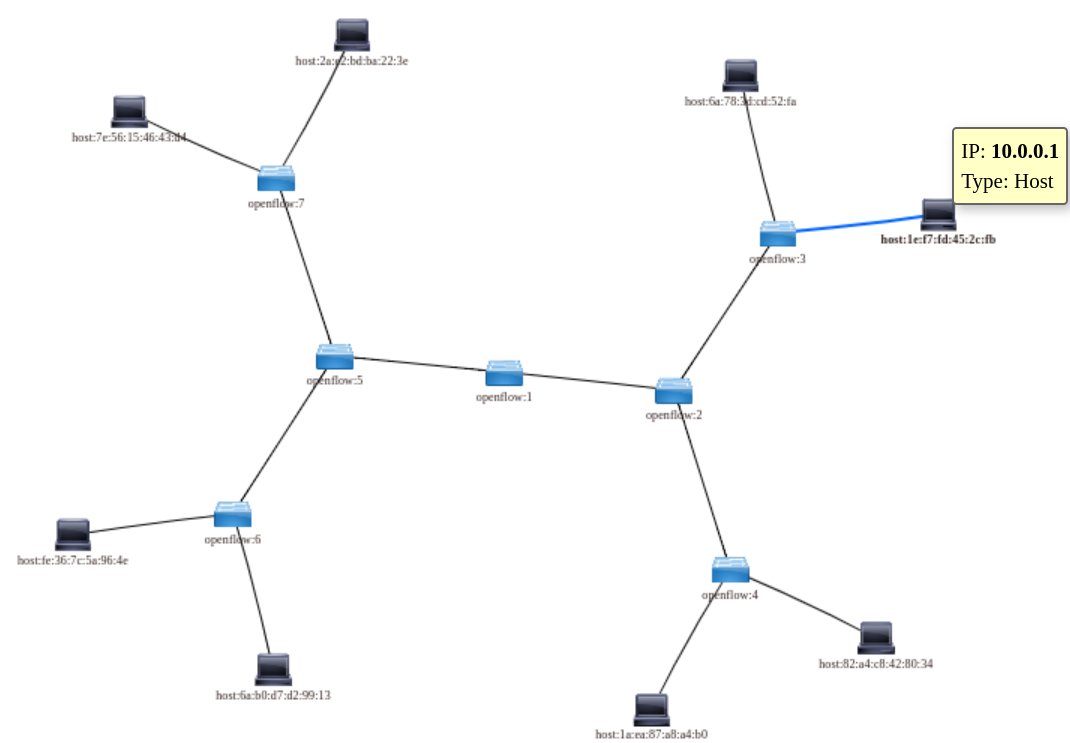
\includegraphics[scale=0.4]{figures/ch5/topo-tree}
	\caption{Tree SDN topology emulated by mininet, and controlled by OpenDayLight Beryllium}
	\label{fig:topo-tree}
\end{figure}

\begin{figure}[!ht]
	\centering
	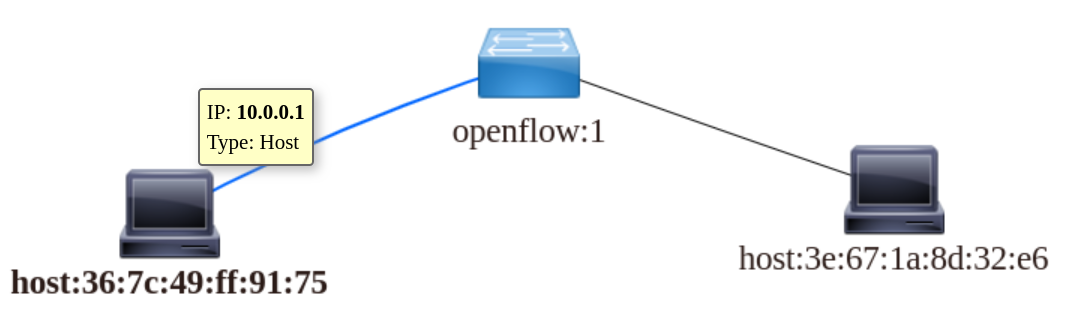
\includegraphics[scale=0.4]{figures/ch5/topo-simple}
	\caption{Single hop SDN topology emulated by mininet, and controlled by OpenDayLight Beryllium}
	\label{fig:topo-simple}
\end{figure}

All Python scripts used to create the scenarios, the Shell Scripts used to automate the tests and capture the traffic, and the Octave scripts to perform all the calculations are available on Github\footnote{\textcolor{red}{github-link}}. To start running the tests, following the tutorial on Github, you should not take more than 10 minutes.

We will perform this testes using SIMITAR \textit{alpha} version, operation as a client on host \textit{h1}, and as a server on all other hosts. As traffic generator engine, we will use D-ITG and Iperf. The operation as a packet injector using Libtins is still unther implementation.

\section{Simitar using Iperf}


\begin{figure}[!ht]
	\centering
	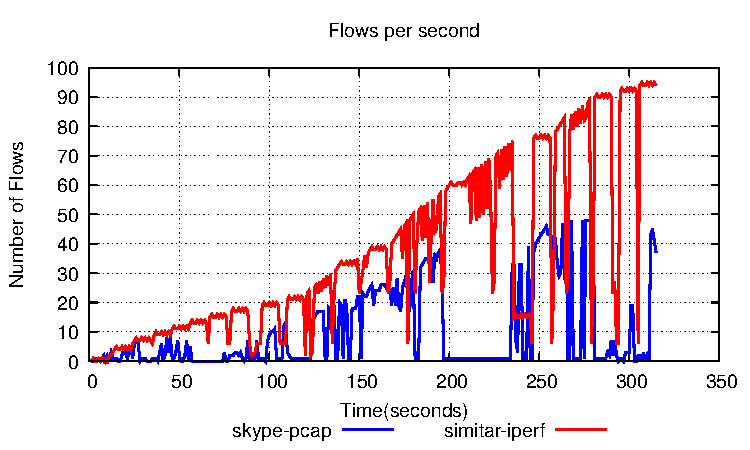
\includegraphics[]{figures/ch5/iperfFlowsPs.pdf}
	\caption{the caption}
	\label{fig:iperfFlowsPs}
\end{figure}

\begin{figure}[!ht]
	\centering
	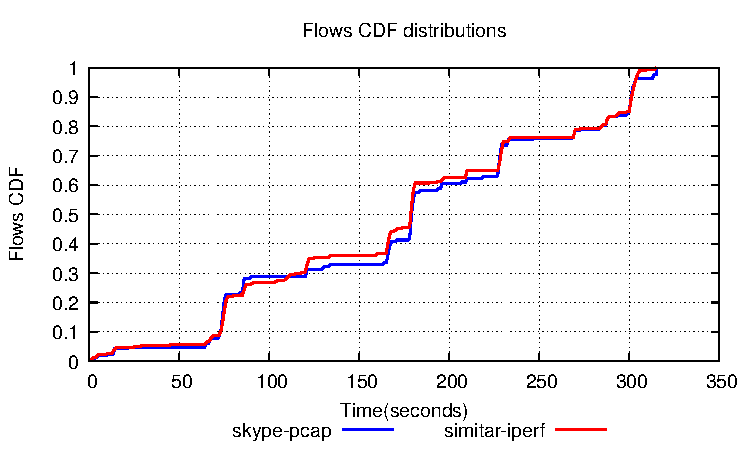
\includegraphics[]{figures/ch5/iperfFlowCdf.pdf}
	\caption{the caption}
	\label{fig:iperfFlowCdf}
\end{figure}

\begin{figure}[!ht]
	\centering
	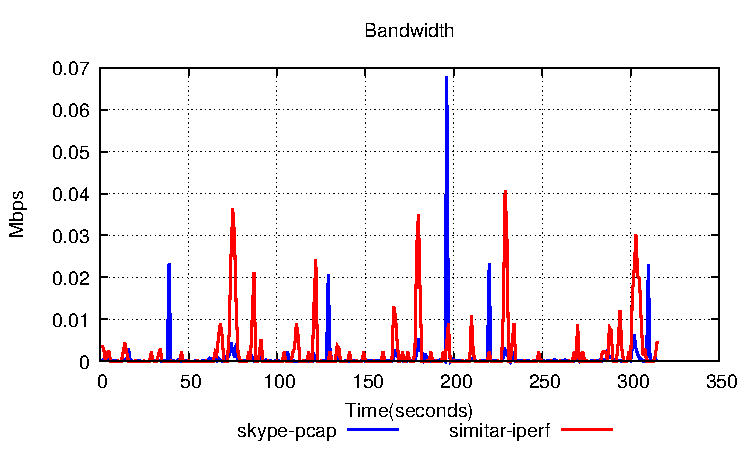
\includegraphics[]{figures/ch5/iperfBandwidth.pdf}
	\caption{the caption}
	\label{fig:iperfBandwidth}
\end{figure}

\begin{figure}[!ht]
	\centering
	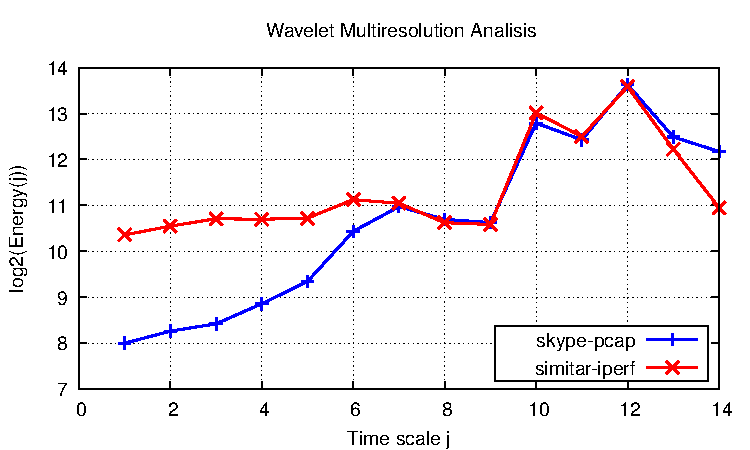
\includegraphics[]{figures/ch5/iperfWaveletMREA.pdf}
	\caption{the caption}
	\label{fig:iperfWaveletMREA}
\end{figure}


\section{Simitar using D-ITG}

\section{Simitar using Libtins}




To evaluate the Scalling profile of the traccic generator, we are usig the same validation used for Swing\cite{swing-paper}: multiresolution energy analysis.


%%%%%%%%%%%%%%%%%%%%%%%%%%%%%%%%%%%%%%%%%%%%%%%%%%%%%%%%%%%%%%%%%%%%%%%%%%%%%%%%
\chapter{Conclusion and Future Work}
\label{ch:conclusion}
%%%%%%%%%%%%%%%%%%%%%%%%%%%%%%%%%%%%%%%%%%%%%%%%%%%%%%%%%%%%%%%%%%%%%%%%%%%%%%%%

\section{Future Work}

%2nd review
In this section we present some ideas for future works and implementation for SIMITAR. On the first section "improving results" we point some approaches for improving the current results. They include calibration of constants, finer control of packet injection, and performance improvement.

\subsection{Improving results}

\subsubsection{Tool calibration}

To imprrove our results, one aproach can be a perform  a deeper study on how calibrate each tool, depending on themain porpose. It can be done first adjusting some parameters and constants of our algorithms and procedures, wich may affect the performance. Some parameters will change the performance  of the tools that support stochastic functions for inter pacekt times:

\begin{itemize}
	
	\item \texttt{DataProcessor::minimumAmountOfPackets}: we just estimate stochastic models for inter-packet times, if the number of flow packets is larger then it. If it is smaller, we just apply the constant model, because with a small sample, the acuracy of any model is poor. Today its value is set to 30.
	
	\item \texttt{DataProcessor::min\_time}: minimum time considered on inter packet times. This is used to avoid inter packet times equals to zero, due the sniffer resolution. This may change the fitting acuracy, wich may change the performance of tools wich use inter-packet time models. Today, this value is $5e-8$. 

\end{itemize}

Others parameters and change of approaches may change the performance for any type of underlying tools or API. They are:

\begin{itemize}

	\item \texttt{DataProcessor::m\_min\_on\_time}: this value controls the small ON time that a \textit{file} can have. This value we can change de precission of the generated traffic. Currently this value is $0.1$s. 
	
	\item \texttt{DataProcessor::m\_session\_cut\_time}:  this member is responsible for defining whaterver a file transfecence still active or has ended. Baically it define the ON and OFF times. 
	
	\item \textit{Control a minimum number of pacekts required for a flow be created}: This would reduce the number of flows created. Since each flow is menaged by a different thread, it can imporrove the performance, reducing overheads. This action should not heavely impact negativally on the throughtput and scalling characteristics, but can increase the precision of the most significant flows. This apply for all underlying traffic-gen engines.
	
	
\end{itemize}



Para extensão do trafego gerado, é necessário um estudo da melhor calibração para cada ferramente, como o D-ITG, Iperf, Libtins, o que pode melhorar os resultados

\subsubsection{SIMITAR as a Packet Injector}

This proposed functionality is still unther implementation, and we are using Libtins API\footnote{\href{http://libtins.github.io/}{http://libtins.github.io/}}. It enable packet crafting and injection at a reasonable performance, adn provide support for many protocols. It is not thread safe, so will require some cares, such as use of mutexes. But will enable a finer controll of packet header contents, packet size, inter packet times and number of pacekts sent. In that way, we expect to achieve better results.  



\begin{figure}[!ht]
	\centering
	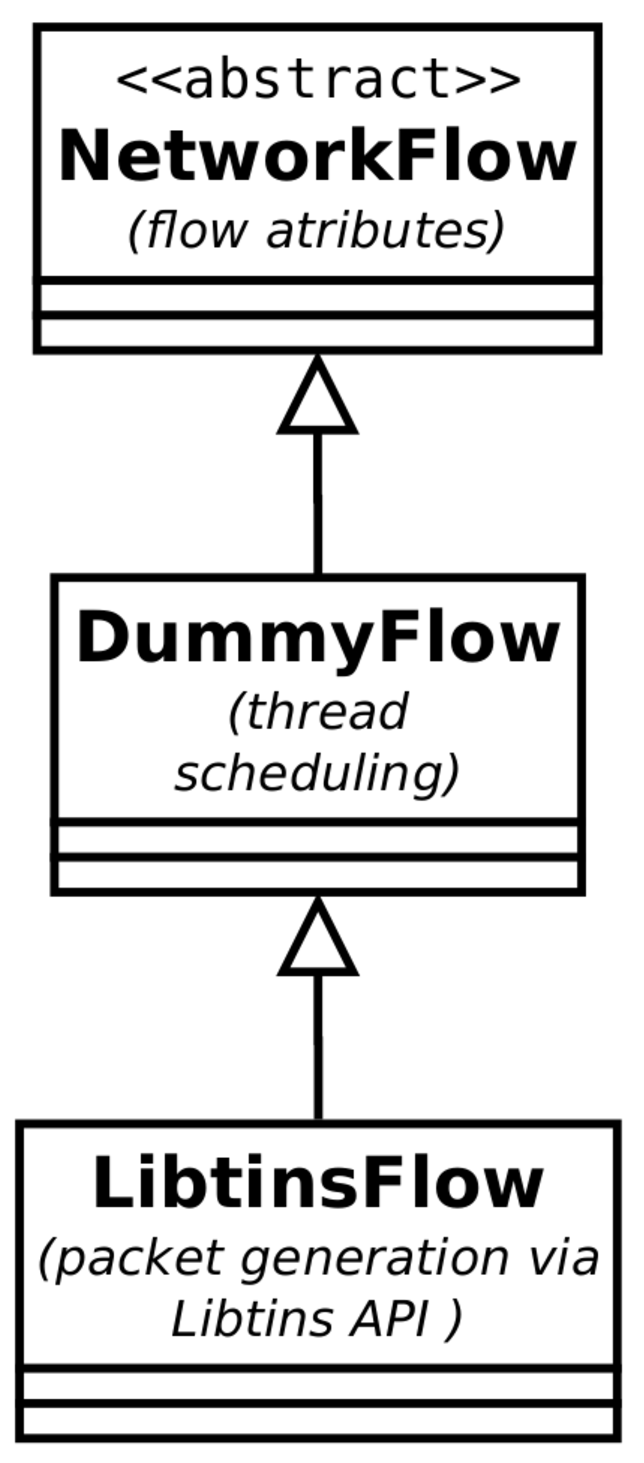
\includegraphics[height=2.0in]{figures/ch6/libtins-flow}
	\caption{Expansion of SIMITAR using Libtins for traffic generation}
	\label{fig:libtins-flow}
\end{figure}

\subsubsection{Traffic generation performance}


\begin{figure}[h!]
	\centering
	\subfloat[DpdkFlow]{
		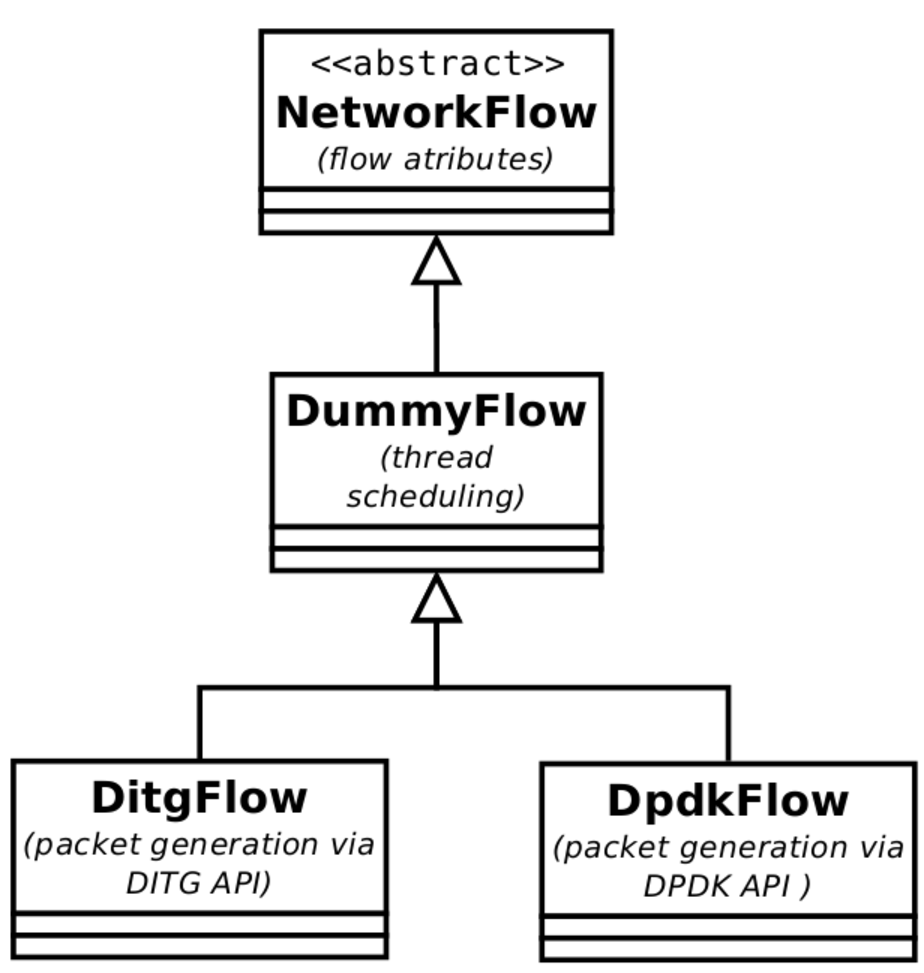
\includegraphics[height=2.0in]{figures/ch6/dpdk-flow}
		\label{fig:dpdk-flow}
	}
	\hspace{0mm}
	\subfloat[DpdkInterface]{
		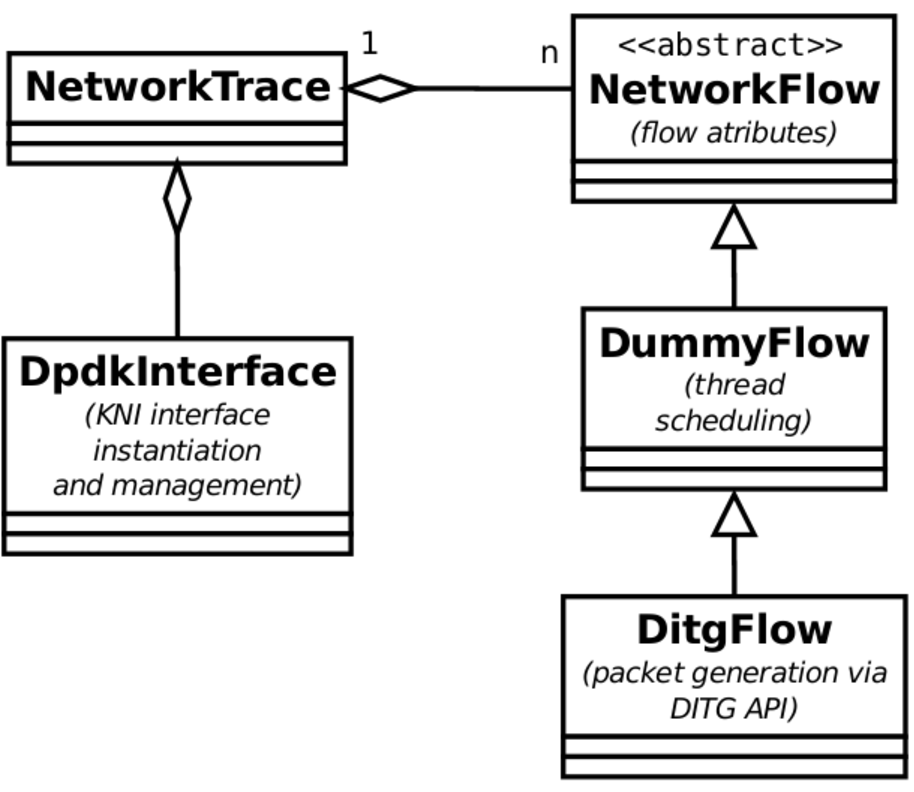
\includegraphics[height=2.0in]{figures/ch6/dpdk-interface}
		\label{fig:dpdk-if}
	}
	\caption{Class diagram for DPDK support expansions. On (a), we have a implementation of traffic generation based on DPDK. On (b) we are using DPDK KNI interfaces.}
	\label{fig:DpdkFlow}
\end{figure}

Some aproaches may be taken to improove the traffic generation performance. One possibility is use DPDK KNI interfaces \footnote{\href{http://dpdk.org/doc/guides/prog_guide/kernel_nic_interface.html}{http://dpdk.org/doc/guides/prog\_guide/kernel\_nic\_interface.html}}. The The DPDK Kernel NIC Interface (KNI) allow applications from the users apace interact with DPDK ports. In this way we may achieve a faster packet processing. 


Another poossibility is use DPDK API craft packets. Using a low level library such for packet generation, we will be able to custom generate packetes, and bypass the Linux network stack (packet acceleration). We present in the figure ~\ref{fig:DpdkFlow} how we could expand our tool to implement an packet generator based on DPDK.

\subsubsection{Thread Menager}

Instead of each flow thread controll individually each sleep and waken times, a better approach would be a separed thread controll and manage all the other thereads life-cycle operation.


\subsubsection{Improving DataProcessor Performance}

Melhorar os algoritimos adicionando técnicas adicionais de modelagem, como condição de parada para o algoritimo gradient descendent, stochastic gradient descendent, entre outros


\subsection{Further Implementations}


\begin{itemize}
	\item \textbf{C++ Sniffer}: Implementing the Sniffer and its SQL queries in C++ should increace its performance.
	
	\item \textbf{Use OpenDayLight REST API for data collection}: Another different approach for data collection ould be use the OpenDayLight REST API to collect data from a SDN OpenFlow switch, instead of a Sniffer. Using the REST API it is possible to stract many statistics from nodes, hosts and ports, such active flows, number of packets matched per flows, packet dopeds, and so on. But, in this case, different featutres would be measured, what would require a development of a new model for traffic generation. On the other hand, many precedures could be reused. 
	
	\item \textbf{SIMITAR Python API}: Currently, SIMITAR only enable the programming of flow traffic generation in C++. Adding Python support for reading NetwrokTrace and NetworkFlow objects would enalbe an easy expantion using Python traffic generation API, without the  need for creating "C++" wrappers.
	
	\item \textbf{Expand SIMITAR}: Expand the SIMITAR support for many other traffic generator tools and APIs, such as MoonGen LUA API, Ostinato Python API, Seagull traffic generator, and many others.
	
		\begin{figure}[!ht]
			\centering
			\includegraphics[height=2.0in]{figures/ch6/pcap-gen}
			\caption{Using SIMITAR for generation synthetic \textit{pcap} files, CTD files: a component schema}
			\label{fig:pcap-gen}
		\end{figure}
	
	\item \textbf{PcapGen: a compact \textit{pcap} lybrary}: This idea reffers to create a component capable of generate synthetic \textit{pcap} files, using Compact Trace Descriptors. This can be implemented using SIMITAR as a packet injector, but in an emulated host interface, using Mininet. Then, the traffic could be collected, using a tool such as TCPDump or Tshark. We present a diagram of this idea in the figure ~\ref{fig:pcap-gen}. This would enable SIMITAR works as trace lybrary for pcap-based benchmark tools.
	

	
	% Oferecer a possibilidade de automatização de medições e testes extendendo a ferramenta
	
	% usar redes neurais para classificação de aplicações
	
\end{itemize}











%\include{docs/06_Limitations}
%\include{docs/chapter}

%\addcontentsline{toc}{chapter}{Conclus\~{a}o}

% ---- ELEMENTOS P\'{O}S-TEXTUAIS ----
\postextual

% ---- Refer\^{e}ncias bibliogr\'{a}ficas ----
%\bibliography{tese}
%\bibliographystyle{ieeetr}
\bibliography{bibliography}
% ---- Ap\^{e}ndices ----

% ---
% Inicia os ap\^{e}ndices
% ---
\begin{apendicesenv}
%
%% Imprime uma p\'{a}gina indicando o in\'{\i}cio dos ap\^{e}ndices
\partapendices

\appendix
\counterwithin{figure}{chapter}
\counterwithin{table}{chapter}

%\include{docs/appendix/01_Appendix}
%\newpage
%\renewcommand{\appendixname}{Appendix}

%\appendix

\chapter{Revision of Probability}
\label{ap:revision-probability}

\section{Stochastic Process}

\section{Random variable}

\section{Probability Distribution Function (PDF)}

\section{Cumulative Distribution Function (CDF)}

\section{Expected value, Variance, Mean and Standard Deviation}

\section{Self-similarity}

\section{Heavy-tailed distributions}

\section{Hurst Exponent}

\section{Maximum likelihood function}

\section{Akaike information criterion}

\section{Bayesian information criterion}

\section{Estimation of parameters of stochastic distributions}

\subsection{Linear Regression and Gradient Descendant Algorithm}

\subsection{Maximum likelihood estimation}

\subsection{Others methods}


%\renewcommand{\appendixname}{Appendix}

\chapter{Chapter 4: Additional Plots}
\chapter{UML Project Diagrams}

\section{Class Diagrams}

\section{Sequence Diagrams}

\chapter{UML Project Diagrams}

\section{Class Diagrams}

\section{Sequence Diagrams}

\chapter{Publications}


\section{IX DCA/FEEC/University of Campinas (UNICAMP) Workshop (EADCA)}
\includepdf[pages=-]{figures/apE/eadca-article2016.pdf}


\section{X DCA/FEEC/University of Campinas (UNICAMP) Workshop (EADCA)}
\includepdf[pages=-]{figures/apE/eadca-article2017.pdf}


\section{Generic Paper}
\includepdf[pages=-]{figures/apE/paper.pdf}



\chapter{TODO List}


\section{Chapter 1 - Introduction - Introduction}


\section{Chapter 2 - Bibliographic Revision }

Liks úteis: 

>> http://www.backtrack-linux.org/forums/showthread.php?t=8740

>> https://sudks.wordpress.com/2016/04/27/tools-traffic-networking/

>> http://www.linuxlinks.com/article/2012042806090428/BenchmarkTools.html

>> http://uperf.org/

\begin{enumerate}

\item TODO \textbf{Geist}\cite{geist-paper} is an application level traffic generator for stress web servers. http://kkant.net/geist/ http://kkant.net/geist/doc/geist\_doc.pdf 

\item TODO https://wiki.fd.io/view/Project\_Proposals/TRex https://github.com/cisco-system-traffic-generator/trex-core
\item TODO TFGEN/MCAST: http://www.pgcgi.com/hptools/
\item TODO Poisson traffic generator http://www.spin.rice.edu/Software/poisson\_gen/
\item TODO http://netsniff-ng.org/ (trafgen)
\item TODO Synthetic self-similar traffic generation http://glenkramer.com/trf\_research.shtml
\item  TODO https://github.com/steerapi/udpgen
\item TODO  http://nutsaboutnets.com/netstress/
\item TODO https://sourceforge.net/projects/ip-packet/
\item TODO PacGen http://sourceforge.net/projects/pacgen/ Packet Forger
\item TODO NTGen http://nssl.eew.technion.ac.il/files/Projects/NTGen\_v2.0/html/index.htm
\item TODO epb - Ethernet Package Bombardier  http://maz-programmersdiary.blogspot.com.br/2012/05/epb-ethernet-package-bombardier.html 


\item (Programa não encontrado) FTP traffic generator: https://pdfs.semanticscholar.org/5756/cf54e46c38dd98c7ad0d5c50deb65a8b33a7.pdf
\item (Programa não encontrado) \textbf{NetSpec}: http://www.cs.columbia.edu/~hgs/internet/traffic-generator.html http://www.ittc.ku.edu/netspec/

\end{enumerate}

\section{Chapter 3 - Architecture}


\section{Chapter 4 - Modeling}


\section{Chapter 5 - Prof of concepts}


\section{Chapter 6 - Usage cases}

\section{Chapter 7 - Conclusion}

%
%% ----------------------------------------------------------
%\chapter{Quisque libero justo}
%% ----------------------------------------------------------
%
%\lipsum[50]
%
%% ----------------------------------------------------------
%\chapter{Nullam elementum urna vel imperdiet sodales elit ipsum pharetra ligula
%ac pretium ante justo a nulla curabitur tristique arcu eu metus}
%% ----------------------------------------------------------
%\lipsum[55-57]
%
\end{apendicesenv}
% ---

% ---- Anexos ----

% ---
% Inicia os anexos - opcional
% ---
%\begin{anexosenv}

% Imprime uma p\'{a}gina indicando o in\'{\i}cio dos anexos
%\partanexos


%\chapter{Primer Anexo}
%---
%\lipsum[30]

% ---
% % %\chapter{Second Anexo}
% ---

% % %\lipsum[31]

% ---
% % %\chapter{Third Anexo}
% ---

% % %\lipsum[32]

%\end{anexosenv}

% ---- INDICE REMISSIVO ----

\printindex

\end{document} 
